%----------------------------------------------------------------------------------------------------------------------------
\graphicspath{{Parti/P04-Travi_rigide/C04_Sistemi_connessioni_eterogenee/Figure/}}
\chapter{Sistemi a connessioni eterogenee}
\label{cap:sistemi_conn_eterogenee}
%----------------------------------------------------------------------------------------------------------------------------


%% ── SOMMARIO (sostituisce righe 7–23) ───────────────────────────────────────
\begin{sommario}
	Si applica la sequenza operativa del \CAPref{cap:assemblaggi_travi}
	a una serie di sistemi a connessioni eterogenee --- la trave
	ramificata con nodi rigidi, l'arco, gli anelli e i sistemi
	compositi a tre cerniere, e le travi su più appoggi (di Gerber
	e continue) --- riconoscendo in ciascuno la gerarchia tra
	sottostrutture portanti e portate. Per ogni esempio si classifica
	il sistema, se ne anticipa qualitativamente la risposta e si
	tracciano i diagrammi completi di $N$, $T$ e $M$; la sola trave
	continua, iperstatica, è discussa nel comportamento e nella
	struttura della soluzione, rinviando al Vol.~II l'analisi
	quantitativa.
\end{sommario}

%----------------------------------------------------------------------------------------------------------------------------
\section*{Considerazioni introduttive}
\label{sec:raccordo_eterogenei}
%----------------------------------------------------------------------------------------------------------------------------

Nei capitoli precedenti della Parte~III sono stati
sviluppati il modello della trave singola e i metodi
per il calcolo delle caratteristiche della sollecitazione
su di essa. Nel \CAPref{cap:assemblaggi_travi} questo
quadro è stato esteso agli assemblaggi di travi,
introducendo le tipologie di connessione --- nodo rigido,
cerniera interna, carrello interno --- e la procedura
operativa per la classificazione dei sistemi. Nella
Parte~II, infine, i concetti di gerarchia strutturale,
di riconoscimento delle sottostrutture isostatiche e di
risoluzione a cascata sono stati sviluppati nel contesto
generale dei sistemi di corpi rigidi.

Il presente capitolo ha un obiettivo specifico e
operativo: sviluppare la procedura per il tracciamento
delle caratteristiche della sollecitazione --- forza
normale $N$, taglio $T$ e momento flettente $M$ ---
su sistemi di travi a \emph{connessioni eterogenee}\index{connessione!eterogenea},
nei quali coesistono connessioni di tipo diverso.
L'analisi viene condotta sull'intera struttura,
così da rendere visibili simultaneamente lo stato
di sollecitazione e i meccanismi di trasferimento
delle forze ai vincoli esterni. Nella risoluzione si fa costante ricorso alle strategie
fondate sulla \emph{gerarchia strutturale} illustrata nel
\PARref{sec:gerarchia}: si riconoscono le sottostrutture
portanti e portate e si risolve a cascata muovendo dalle
porzioni \emph{portate} --- risolubili in modo autonomo non
appena se ne assumano come vincoli gli appoggi sulle portanti
--- verso le porzioni \emph{portanti} che le sorreggono,
per ricomporre infine le azioni interne sull'intero
assemblaggio.

I sistemi trattati si dividono in due gruppi. Il primo
comprende sistemi \emph{isostatici} --- la trave ramificata
con nodi rigidi, l'arco a tre cerniere, gli anelli a tre
cerniere, i sistemi compositi a tre cerniere e le travi di
Gerber --- per i quali la procedura si articola nei quattro
passi sviluppati nella \SECref{sec:sequenza_operativa} e
applicati sistematicamente negli esempi che seguono.
Il secondo è costituito dalla \emph{trave continua}, sistema
iperstatico di grado $n_a - 2$: per essa si discutono la
classificazione, il comportamento statico e la struttura
della soluzione, senza svilupparne l'analisi quantitativa,
rinviata al Vol.~II.

La trattazione delle travi su più appoggi segue un ordine
preciso: prima le travi di Gerber, poi le travi continue.
La ragione è metodologica: in assenza del legame costitutivo
--- non ancora disponibile in questa Parte --- la trave
continua resta staticamente indeterminata, mentre la trave
di Gerber, grazie alle cerniere interne, è risolubile con i
soli strumenti della statica. Esaurire dapprima i casi
interamente risolubili consente poi di mettere in evidenza,
per confronto, in che senso la continuità introduca
l'iperstaticità. Tale confronto, sviluppato nella
\SECref{sec:travi_piu_appoggi}, mostra come l'inserimento di
cerniere interne in posizioni opportune trasformi un sistema
iperstatico in uno isostatico a parità di schema geometrico
esterno.



%----------------------------------------------------------------------------------------------------------------------------
\section{La sequenza operativa}
\label{sec:sequenza_operativa}
%----------------------------------------------------------------------------------------------------------------------------

L'analisi di un sistema di travi a connessioni
eterogenee segue una sequenza in quattro passi che
generalizza al caso degli assemblaggi la procedura
già sviluppata per la trave singola
(\CAPref{cap:Diagrammi_CS}) e per i sistemi di
corpi rigidi (\CAPref{cap:classificazione_sol_SCR}).
La sequenza è valida per qualsiasi sistema isostatico
a connessioni eterogenee, indipendentemente dalla
sua complessità geometrica.

%............................................................................................................................
\paragraph{Passo 1 --- Equilibrio globale e
	reazioni vincolari esterne.}
%............................................................................................................................

Si applica l'equilibrio alla struttura trattata
come un unico corpo rigido, considerando i soli
vincoli esterni e i carichi applicati. Le tre
equazioni cardinali della statica --- due di
traslazione e una di momento --- forniscono le
reazioni vincolari esterne quando il sistema è
isostatico esternamente.

In alcuni sistemi --- come l'arco a tre cerniere
o i sistemi con gerarchia strutturale esplicita
--- le sole equazioni globali non sono sufficienti
a determinare tutte le reazioni esterne. In questi
casi occorre integrare l'equilibrio globale con
l'equilibrio di sottosistemi opportunamente isolati,
sfruttando le condizioni imposte dalle connessioni
interne (ad esempio la condizione $M = 0$ alla
cerniera interna). L'ordine di risoluzione è
imposto dalla gerarchia strutturale: i sottosistemi
portati si risolvono per primi e le loro reazioni
diventano carichi noti per i sottosistemi portanti.

\begin{oss}
	Le condizioni di raccordo alle connessioni
	interne riguardano le caratteristiche della
	sollecitazione \emph{trasmesse dalla
		connessione}. Se una forza o una coppia
	attiva è applicata a una delle travi
	convergenti nella sezione di connessione,
	essa entra nell'equilibrio di quella trave
	senza alterare la natura della connessione:
	la caratteristica non trasmessa rimane nulla
	sulla sezione di estremità di ciascuna trave,
	ma il valore della caratteristica trasmessa
	è modificato dalla presenza del carico attivo
	su quella trave. La distinzione tra grandezze
	\emph{reattive} --- trasmesse dalla connessione
	--- e forze \emph{attive} --- applicate a una
	delle travi --- è essenziale per l'impostazione
	corretta dell'equilibrio in corrispondenza
	di qualsiasi tipo di svincolo interno.
\end{oss}

%............................................................................................................................
\paragraph{Passo 2 --- Gerarchia interna e azioni
	alle connessioni.}
%............................................................................................................................

Note le reazioni vincolari esterne, si scompone
la struttura nelle travi componenti e si individua
la \emph{gerarchia interna}\index{gerarchia strutturale}: l'ordine in cui le
travi possono essere risolte progressivamente,
partendo da quelle con azioni già completamente
note alle estremità e risalendo la catena
strutturale.

Il punto di partenza è sempre una trave con
almeno un'estremità libera o vincolata al suolo
in modo noto: su di essa le azioni di estremità
sono determinate dall'equilibrio. Le azioni
così calcolate diventano note per la trave
adiacente connessa in quel punto, che può
essere risolta a sua volta. Il procedimento
si ripete fino a esaurire tutte le travi
componenti.

Su ciascuna trave isolata si riportano:
\begin{itemize}
	\item i \emph{carichi attivi}\index{carico!attivo} direttamente
	applicati alla trave (forze concentrate,
	coppie, carichi distribuiti);
	\item le \emph{reazioni vincolari esterne}
	nei nodi vincolati al suolo, già note
	dal Passo~1;
	\item le \emph{azioni alle connessioni
		interne}, determinate progressivamente
	nell'ordine imposto dalla gerarchia,
	con verso opposto a quelle agenti sulla
	trave adiacente per il principio di
	azione e reazione.
\end{itemize}

La natura delle azioni alle connessioni dipende
dal tipo di svincolo:
\begin{itemize}
	\item \emph{Cerniera interna}: trasmette
	forza normale $N$ e taglio $T$, ma non
	momento flettente; la condizione $M = 0$
	vale per ciascuna delle travi convergenti
	nel nodo. Le incognite sono le due componenti
	della reazione nella cerniera.
	
	\item \emph{Nodo rigido}: trasmette
	integralmente $N$, $T$ e $M$, con la
	trasformazione dovuta al cambio di sistema
	locale tra travi di orientamento diverso.
	Le incognite sono le tre componenti della
	reazione al nodo.
	
	\item \emph{Carrello interno trasversale}:
	trasmette il solo taglio $T$; la forza
	normale $N$ e il momento $M$ sono nulli.
	L'unica incognita è la componente
	trasversale della reazione.
	
	\item \emph{Carrello interno longitudinale}:
	trasmette il solo sforzo normale $N$;
	taglio $T$ e momento $M$ sono nulli.
	L'unica incognita è la componente
	longitudinale della reazione.
\end{itemize}

\begin{oss}
	Nei nodi rigidi tra travi di orientamento
	diverso la trasformazione delle caratteristiche
	della sollecitazione tra sistemi locali richiede
	attenzione particolare. Se due travi convergono
	rigidamente in un nodo con angolo $\alpha$ tra
	i rispettivi assi, le componenti $N$ e $T$
	di una trave si proiettano su $N$ e $T$
	dell'altra secondo le relazioni di rotazione
	già introdotte nel \CAPref{cap:assemblaggi_travi}.
	Il momento $M$ è invece uno scalare invariante
	per rotazioni nel piano e si trasmette senza
	trasformazione.
\end{oss}

%............................................................................................................................
\paragraph{Passo 3 --- Fibre inferiori e
	convenzioni di segno.}
%............................................................................................................................

Prima di procedere al tracciamento dei diagrammi
si stabilisce, per ciascun tratto della struttura,
la \emph{fibra inferiore}\index{fibra inferiore}: il lato della trave
assunto come riferimento per la convenzione di
segno del momento flettente, tracciato con linea
tratteggiata nella figura complessiva della
struttura. La fibra inferiore definisce il
\emph{verso di percorrenza} di ciascun tratto
--- dal nodo iniziale al nodo finale --- e con
esso il sistema locale $(z,\,y)$ del tratto:
asse $z$ orientato lung\o il verso di percorrenza,
asse $y$ perpendicolare dal lato della fibra
inferiore.

La scelta della fibra inferiore è una convenzione,
ma deve essere \emph{coerente} sull'intera struttura.
Il criterio di larga massima è il seguente: per i
tratti orizzontali si assume la fibra inferiore
coincidente con l'intradosso geometrico; per i
tratti verticali e inclinati si estende questa
scelta in modo che il verso di percorrenza risulti
continuo e logico nell'insieme della struttura.

Le convenzioni di segno che ne derivano sono:
\begin{itemize}
	\item il \emph{momento flettente} positivo
	si traccia sempre dal lato della fibra
	inferiore --- questa è l'unica convenzione
	non a discrezione dell'operatore;
	\item il \emph{taglio} e la \emph{forza
		normale} positivi si tracciano dal lato
	del semiasse scelto dall'operatore; la
	scelta è libera ma deve rimanere coerente
	per tutti i tratti allineati o connessi
	tra loro.
\end{itemize}

%............................................................................................................................
\paragraph{Passo 4 --- Tracciamento dei diagrammi
	$N$, $T$, $M$ sull'intera struttura.}
%............................................................................................................................

Su ciascuna trave componente, note tutte le azioni di estremità e i carichi applicati, si tracciano 
i diagrammi $N$, $T$, $M$ con il metodo già sviluppato per la trave singola con il \emph{metodo per equivalenza} 
già sviluppato per la trave singola (\CAPref{cap:Diagrammi_CS}):

\begin{itemize}
	\item in assenza di carichi distribuiti,
	$N$ e $T$ sono uniformi e $M$ è lineare
	su ciascun tratto;
	
	\item sotto carico distribuito uniforme,
	$N$ e $T$ sono lineari e $M$ è parabolico;
	
	\item sotto carico distribuito $p(z)$ a legge lineare
	(triangolare), $T$ è parabolico e $M$ è cubico;
	nel punto dove il carico si annulla la tangente
	al diagramma di $T$ è parallela all'asse della
	trave; analogamente, nel punto dove $T$ si annulla
	la tangente al diagramma di $M$ è parallela
	all'asse della trave.
	
	\item in corrispondenza di una forza
	concentrata, $N$ e $T$ presentano un salto pari
	alle componenti assiale e trasversale della forza;
	$M$ è continuo ma presenta una variazione di pendenza;
	
	\item in corrispondenza di una coppia
	concentrata, $M$ presenta un salto pari
	all'intensità della coppia; $N$ e $T$
	sono continui.
\end{itemize}

I diagrammi delle singole travi si giustappongono
per ottenere il quadro delle caratteristiche
della sollecitazione sull'intera struttura.
Le condizioni di raccordo alle connessioni
interne --- annullamento di $M$ alla cerniera,
continuità di $M$ al nodo rigido (con eventuale
trasformazione tra sistemi locali), annullamento
della caratteristica non trasmessa al carrello
--- si leggono direttamente sul diagramma
globale come verifica della correttezza
dell'analisi.

La lettura del diagramma globale consente
di identificare il \emph{meccanismo di
	trasferimento delle forze}: quali travi
lavorano prevalentemente a flessione,
quali a taglio, quali a sforzo normale,
e come i carichi fluiscono verso i vincoli
esterni.

\begin{oss}
	La sequenza appena descritta non abbandona il
	\emph{metodo per equivalenza} adottato per la trave
	singola (\CAPref{cap:Diagrammi_CS}): lo riorganizza.
	Isolata ciascuna trave componente con le azioni di
	estremità note (Passo~2), il tracciamento dei suoi
	diagrammi (Passo~4) è esattamente l'equivalenza già
	vista --- la caratteristica in una sezione come
	risultante delle forze agenti su uno dei due tratti,
	guardando a sinistra o a destra.
	
	In linea di principio l'equivalenza si potrebbe
	applicare \emph{globalmente}, riducendo alla sezione
	in esame tutto ciò che sta da una parte dell'intero
	assemblaggio. Per i sistemi di travi, però, questa via
	è più insidiosa: la parte ``a sinistra'' o ``a destra''
	può comprendere più travi di orientamento diverso e
	connessioni interne, e le forze vanno trasportate e
	proiettate nel sistema locale della sezione attraverso
	la geometria. L'isolamento gerarchico delle travi
	(Passo~2) evita questa difficoltà, riconducendo ogni
	tratto al caso già padroneggiato della trave singola.
	I due approcci non si contraddicono: la gerarchia
	organizza il calcolo, l'equivalenza ne è il principio,
	applicato trave per trave.
\end{oss}

\begin{oss}
	Le equazioni indefinite di equilibrio locale
	$N' = -q$, $T' = -p$, $M' = T$ --- l'ultima valida in assenza di coppie distribuite ---
	forniscono una regola generale per la lettura
	qualitativa dei diagrammi: nel punto in cui
	$q_0 = 0$ la tangente al diagramma di $N$
	è parallela all'asse della trave; nel punto
	in cui $q = 0$ la tangente al diagramma di $T$
	è parallela all'asse della trave; nel punto
	in cui $T = 0$ la tangente al diagramma di $M$
	è parallela all'asse della trave.
	In presenza di forze concentrate, $N$ e $T$
	presentano un salto pari alle componenti
	assiale e trasversale della forza; $M$ è
	continuo ma con variazione di pendenza.
	In presenza di coppie concentrate, $M$
	presenta un salto pari all'intensità della
	coppia; $N$ e $T$ sono continui.
\end{oss}

\begin{oss}
	I punti di momento nullo --- dove il
	diagramma di $M$ si annulla --- hanno
	un significato strutturale preciso:
	in quei punti la trave non trasmette
	momento flettente e si comporta
	localmente come una cerniera. Nei
	sistemi isostatici questi punti sono
	imposti dalla topologia delle connessioni
	(le cerniere interne); nei sistemi
	iperstatici dipendono anche dalla
	rigidezza relativa degli elementi e
	non sono determinabili senza i metodi
	del Vol.~II.
\end{oss}


%----------------------------------------------------------------------------------------------------------------------------
\section{Trave ramificata con nodi rigidi}
\label{sec:trave_ramificata}
%----------------------------------------------------------------------------------------------------------------------------

Come primo esempio si considera la trave ramificata\index{trave!ramificata}
piana con connessioni rigide illustrata nella
\FIGref{fig:trave_ramificata}. La struttura è
composta da quattro travi --- $AB$, $BC$, $BD$
e $DE$ --- collegate da un nodo a tre vie in $B$
e un nodo a due vie in $D$, entrambi rigidi.
La cerniera in $A$ ($m = 2$) e il carrello
verticale in $C$ ($m = 1$) forniscono i tre
vincoli esterni necessari per l'isostaticità.
I carichi applicati sono una forza concentrata
$p\ell$ nel punto medio di $AB$ e un carico
distribuito uniforme di intensità $p$ sul
tratto $DE$.

%%%%%%%%%%%%%%%%%%%%%%%%%%%%%%%%%%%%%%%%%%%
\begin{figure}[htbp]
	\centering
	\begin{tikzpicture}[
		trave/.style={line width=2.0pt, line cap=round,
			line join=round, black},
		fibra/.style={line width=0.8pt, dashed, gray!50,
			line cap=round},
		carico/.style={->, >=stealth, line width=1.2pt, black},
		reaz/.style={->, >=stealth, line width=1.2pt, gray!70},
		terra/.style={line width=0.8pt, black},
		nodoV/.style={circle, fill=white, draw=black,
			inner sep=0pt, minimum size=6pt,
			line width=0.9pt},
		quota/.style={|<->|, >=stealth, thin, gray!60},
		]
		
		\def\L{3.0}   % lunghezza asta in cm
		
		%% ── Coordinate nodali ───────────────────────────────
		\coordinate (A) at (0,    0);
		\coordinate (B) at (\L,   0);
		\coordinate (C) at (2*\L, 0);
		\coordinate (D) at (\L,   \L);
		\coordinate (E) at (2*\L, \L);
		
		%		%% ── Fibre inferiori (tratteggiate) ──────────────────
		%		%% Tratti orizzontali: sotto la trave
		%		\draw[fibra] ($(A)+(0,-0.12)$)   -- ($(B)+(0,-0.12)$);
		%		\draw[fibra] ($(B)+(0,-0.12)$)   -- ($(C)+(0,-0.12)$);
		%		\draw[fibra] ($(D)+(0,-0.12)$)   -- ($(E)+(0,-0.12)$);
		%		%% Tratto verticale BD: a destra della trave
		%		\draw[fibra] ($(B)+(0.12,0.00)$) -- ($(D)+(0.12,0.00)$);
		
		%% ── Travi ───────────────────────────────────────────
		\draw[trave] (A) -- (B);
		\draw[trave] (B) -- (C);
		\draw[trave] (B) -- (D);
		\draw[trave] (D) -- (E);
		
		%% ── Vincolo: cerniera in A ──────────────────────────
		\draw[terra] (A) -- ++(-0.30,-0.52) -- ++(0.60,0) -- cycle;
		\draw[terra] (-0.40,-0.52) -- (0.40,-0.52);
		\foreach \x in {-0.34,-0.18,-0.02,0.14,0.30}
		\draw[very thin, black] (\x,-0.52) -- ++(-0.12,-0.15);
		
		%% ── Vincolo: carrello verticale in C ────────────────
		\draw[terra] (C) -- ++(-0.30,-0.42) -- ++(0.60,0) -- cycle;
		\draw[terra] ($(C)+(-0.40,-0.42)$) -- ($(C)+(0.40,-0.42)$);
		\draw[terra] ($(C)+(-0.22,-0.58)$) circle (3.2pt);
		\draw[terra] ($(C)+( 0.22,-0.58)$) circle (3.2pt);
		\draw[terra] ($(C)+(-0.40,-0.74)$) -- ($(C)+(0.40,-0.74)$);
		\foreach \x in {-0.34,-0.18,-0.02,0.14,0.30}
		\draw[very thin, black] ($(C)+(\x,-0.74)$) -- ++(-0.12,-0.15);
		
		%% ── Nodi vincolati: cerchio bianco sopra i vincoli ──
		\node[nodoV] at (A) {};
		\node[nodoV] at (C) {};
		
		%% ── Reazioni vincolari (code in A e C, punte in alto)
		\draw[reaz]
		($(A)+(0,0.00)$) -- ($(A)+(0,1.00)$)
		node[midway, right, font=\small, gray!80]
		{$V_A$};
		\draw[reaz]
		($(C)+(0,0.00)$) -- ($(C)+(0,1.00)$)
		node[midway, right, font=\small, gray!80]
		{$Y_C$};
		\draw[reaz]
		($(A)+(-1.00,0)$) -- ($(A)+(0,0)$)
		node[midway, below, font=\small, gray!80]
		{$H_A $};
		
		%% ── Carico concentrato su AB ────────────────────────
		\draw[carico]
		($(A)!0.5!(B)+(0,1.10)$) -- ($(A)!0.5!(B)+(0,0.08)$);
		\node[above, font=\small]
		at ($(A)!0.5!(B)+(0,1.10)$) {$p\ell$};
		
		%% ── Carico distribuito su DE ────────────────────────
		\draw[black, line width=0.8pt]
		($(D)+(0,0.70)$) -- ($(E)+(0,0.70)$);
		\foreach \t in {0.00,0.17,0.34,0.50,0.67,0.84,1.00} {
			\draw[carico, line width=0.8pt]
			($(D)!\t!(E)+(0,0.70)$) -- ($(D)!\t!(E)+(0,0.08)$);
		}
		%% Linea inferiore del carico distribuito (altezza punte)
		\draw[black, line width=0.5pt]
		($(D)+(0,0.08)$) -- ($(E)+(0,0.08)$);
		\node[above, font=\small]
		at ($(D)!0.5!(E)+(0,0.70)$) {$p$};
		
		%% ── Etichette nodi ──────────────────────────────────
		\node[above left,  font=\small] at (A) {$A$};
		\node[above left,       font=\small] at (B) {$B$};
		\node[above left, font=\small] at (C) {$C$};
		\node[left,        font=\small] at (D) {$D$};
		\node[right,       font=\small] at (E) {$E$};
		
		%% ── Quote ───────────────────────────────────────────
		%% Quota AB: sotto la struttura
		\draw[quota] ($(A)+(0,-1.30)$) -- ($(B)+(0,-1.30)$)
		node[midway, above, font=\small] {$\ell$};
		%% Quota BC: sotto la struttura
		\draw[quota] ($(B)+(0,-1.30)$) -- ($(C)+(0,-1.30)$)
		node[midway, above, font=\small] {$\ell$};
		%% Quota BD: a sinistra della reazione V_A,
		%% posizionata tra x=-1.20 e x=-1.20+\L
		\draw[quota] (-1.20, 0) -- (-1.20, \L)
		node[midway, right, font=\small] {$\ell$};
		
	\end{tikzpicture}
	\caption{Trave ramificata con connessioni rigide in
		$B$ e $D$. Cerniera in $A$, carrello
		verticale in $C$. Carico concentrato $p\ell$
		nel punto medio di $AB$; carico distribuito
		uniforme $p$ sul tratto $DE$.
		Le linee tratteggiate indicano le fibre inferiori
		dei quattro tratti.}
	\label{fig:trave_ramificata}
\end{figure}
%%%%%%%%%%%%%%%%%%%%%%%%%%%%%%%%%%%%%%%%%%%

\noindent\textbf{Classificazione.}
Per ispezione diretta, la struttura nel suo insieme
si comporta come una trave appoggiata: la cerniera
in $A$ e il carrello in $C$ sono i soli vincoli
al suolo e forniscono esattamente tre reazioni
($H_A$, $V_A$, $Y_C$), sufficienti a equilibrare
un sistema piano generico. Il sistema è quindi
isostatico esternamente e, avendo connessioni
interne tutte rigide senza maglie chiuse, è
internamente isostatico.

Il conteggio di Müller-Breslau conferma questa
ispezione. Con $n_e = 4$ travi, $m_\text{est} = 3$
e molteplicità interna $m_\text{int} = 3(3-1) +
3(2-1) = 6 + 3 = 9$ (nodo $B$ a tre vie e nodo
$D$ a due vie, entrambi rigidi):
\[
\nu = 3n_e - m_\text{int} - m_\text{est}
= 12 - 9 - 3 = 0.
\]
La struttura è isostatica. $\quad\checkmark$


%..........................................................................
\paragraph{Passo 1 --- Equilibrio globale e
	reazioni vincolari esterne.}
%..........................................................................

Si applica l'equilibrio globale trattando la
struttura come un unico corpo rigido.
Le reazioni sono $H_A$ e $V_A$ in $A$
(cerniera) e $Y_C$ in $C$ (carrello verticale).
Il carico distribuito su $DE$ ha risultante
$p\ell$ applicata nel punto medio di $DE$,
di coordinate $\bigl(\tfrac{3}{2}\ell,\,\ell\bigr)$.

\noindent Equilibrio alla traslazione orizzontale:
\[
\sum H = 0:\quad H_A = 0.
\]

\noindent Equilibrio alla rotazione attorno ad $A$:
\[
\sum \mu_A = 0:\quad
Y_C \cdot 2\ell
- p\ell \cdot \frac{\ell}{2}
- p\ell \cdot \frac{3\ell}{2} = 0
\;\Rightarrow\;
Y_C = p\ell.
\]

\noindent Equilibrio alla traslazione verticale:
\[
\sum V = 0:\quad
V_A = p\ell.
\]

Le reazioni vincolari sono:
\[
H_A = 0, \qquad V_A = p\ell, \qquad Y_C = p\ell.
\]

In questo esempio le sole equazioni globali
sono sufficienti a determinare le reazioni
esterne, perché il sistema è isostatico
esternamente con tre vincoli e tre equazioni
cardinali. Nei sistemi con gerarchia interna
più complessa --- come l'arco a tre cerniere
--- sarà necessario integrare l'equilibrio
globale con quello di sottosistemi isolati.

%..........................................................................
\paragraph{Passo 2 --- Gerarchia interna e azioni
	alle connessioni.}
%..........................................................................

Si scompone la struttura nelle quattro travi
componenti $AB$, $BC$, $BD$, $DE$ e si
individua la gerarchia interna, ossia l'ordine
in cui le travi possono essere risolte
progressivamente.

La trave $DE$ ha l'estremità $E$ libera: su
di essa tutte le caratteristiche sono nulle.
È quindi il punto di partenza naturale della
gerarchia. Note le azioni in $D$ sul tratto
$DE$, queste diventano note per il tratto $BD$
connesso rigidamente in $D$. A sua volta,
note le azioni in $B$ sul tratto $BD$, insieme
alle reazioni esterne già note in $A$ e $C$,
si determinano le azioni in $B$ sui tratti
$AB$ e $BC$.



\medskip
\noindent\textit{Trave $DE$ (orizzontale,
	lunghezza $\ell$, estremità $E$ libera).}

Su $DE$ agisce il carico distribuito $p$
verso il basso. A distanza $x$ da $E$:
\[
T(x) = px, \qquad M(x) = -\frac{px^2}{2}.
\]
In $D$ (per $x = \ell$):
\[
N_D^{DE} = 0, \qquad
T_D^{DE} = p\ell, \qquad
M_D^{DE} = -\frac{p\ell^2}{2}.
\]

\medskip
\noindent\textit{Trave $BD$ (verticale,
	lunghezza $\ell$, da $B$ verso $D$).}

Il nodo $D$ è rigido: le azioni che $DE$
trasmette a $BD$ in $D$ si ricavano per
azione e reazione, tenendo conto del cambio
di sistema locale da orizzontale a verticale.
Nel sistema locale di $BD$ (asse $z$ verticale
verso l'alto, asse $y$ orizzontale):
\[
\begin{aligned}
	N_D^{BD} &= -T_D^{DE} = -p\ell
	\quad\text{(compressione)},
	\qquad
	T_D^{BD} = N_D^{DE} = 0,\\[4pt]
	M_D^{BD} &= M_D^{DE} = -\frac{p\ell^2}{2}.
\end{aligned}
\]
Il tratto $BD$ è privo di carichi: $N$ e $T$
sono costanti, $M$ è lineare. In $B$:
\[
N_B^{BD} = -p\ell, \qquad
T_B^{BD} = 0, \qquad
M_B^{BD} = -\frac{p\ell^2}{2}.
\]

\medskip
\noindent\textit{Trave $AB$ (orizzontale,
	lunghezza $\ell$).}

Su $AB$ agiscono: la reazione in $A$
($H_A = 0$, $V_A = p\ell$) e il carico
concentrato $p\ell$ verso il basso in
$(\ell/2,\,0)$. Le azioni in $B$ si
determinano dall'equilibrio del tratto:
\[
N_B^{AB} = 0, \qquad
T_B^{AB} = 0, \qquad
M_B^{AB} = \frac{p\ell^2}{2}.
\]

\medskip
\noindent\textit{Trave $BC$ (orizzontale,
	lunghezza $\ell$).}

Su $BC$ agisce la reazione in $C$
($Y_C = p\ell$). Le azioni in $B$ si
determinano dall'equilibrio del tratto:
\[
N_B^{BC} = 0, \qquad
T_B^{BC} = p\ell, \qquad
M_B^{BC} = p\ell^2.
\]
La \FIGref{fig:corpi_liberi_ramificata} raccoglie
i quattro corpi liberi con le azioni alle
connessioni interne così determinate.

\medskip
\noindent\textit{Verifica: equilibrio del nodo $B$.}

\noindent Il nodo $B$ riceve le azioni dai tre tratti
convergenti. Nel riferimento globale $(x,\,y)$:

\noindent Da $AB$ (verso opposto):
$F_x = 0$, $F_y = 0$, $M = -p\ell^2/2$.

\noindent Da $BC$ (verso opposto):
$F_x = 0$, $F_y = p\ell$, $M = p\ell^2$.

\noindent Da $BD$ ($N$ nella direzione $y$,
$T$ nella direzione $x$, verso opposto):
$F_x = 0$, $F_y = -p\ell$, $M = -p\ell^2/2$.

\[
\sum H = 0, \quad
\sum V = p\ell - p\ell = 0, \quad
\sum M = -\frac{p\ell^2}{2} + p\ell^2
- \frac{p\ell^2}{2} = 0.
\quad\checkmark
\]

\begin{oss}
	La verifica al nodo $B$ mostra come il
	momento si distribuisca tra i tre tratti
	convergenti: il momento $p\ell^2$ proveniente
	da $BC$ si ripartisce tra $AB$ e $BD$,
	ciascuno dei quali riceve $p\ell^2/2$
	con segno opposto. Il nodo rigido funziona
	come un \emph{distributore di momenti}:
	la ripartizione è imposta dall'equilibrio
	e non dipende dalla rigidezza, come è
	proprio dei sistemi isostatici.
\end{oss}

\begin{figure}[htbp]
	\centering
	\resizebox{\textwidth}{!}{%
		\begin{tikzpicture}[
			trave/.style={line width=2.2pt, line cap=round, line join=round, black},
			terra/.style={line width=0.7pt, black},
			nodoV/.style={circle, fill=white, draw=black, inner sep=0pt,
				minimum size=5pt, line width=0.8pt},
			carico/.style={->, >=stealth, line width=1.0pt, black},
			reaz/.style={->, >=stealth, line width=1.0pt, gray!60},
			forza/.style={->, >=stealth, line width=1.0pt, black},
			blob/.style={draw=gray!45, fill=gray!10, line width=0.7pt,
				rounded corners=14pt},
			]
			
			\def\L{3.2}
			\def\sc{0.65}
			\def\rm{0.38}  % raggio archi momento — più grande per visibilità
			
			%% Macro arco ORARIO (~200° CCW, wraps RIGHT side)
			%% Visivamente: C aperta a sinistra, freccia punta in basso-sinistra in cima
			\newcommand{\arcORA}[1]{%
				\draw[->,>=stealth,line width=0.9pt]
				($(#1)+({\rm*cos(-100)},{\rm*sin(-100)})$) arc(-100:100:\rm);
			}
			%% Macro arco ANTIORARIO (~200° CCW, wraps LEFT side)
			%% Visivamente: C aperta a destra, freccia punta in basso-destra in fondo
			\newcommand{\arcANTI}[1]{%
				\draw[->,>=stealth,line width=0.9pt]
				($(#1)+({\rm*cos(80)},{\rm*sin(80)})$) arc(80:280:\rm);
			}
			%% Macro arco ANTIORARIO (~200° CCW, wraps LEFT side)
			%% Visivamente: C aperta a destra, freccia punta in basso-destra in fondo
			\newcommand{\arcANTIAP}[1]{%
				\draw[<-,>=stealth,line width=0.9pt]
				($(#1)+({\rm*cos(80)},{\rm*sin(80)})$) arc(80:280:\rm);
			}
			%% Macro arco ORARIO (~200° CCW, wraps RIGHT side)
			%% Visivamente: C aperta a sinistra, freccia punta in basso-sinistra in cima
			\newcommand{\arcORAAP}[1]{%
				\draw[<-,>=stealth,line width=0.9pt]
				($(#1)+({\rm*cos(-100)},{\rm*sin(-100)})$) arc(-100:100:\rm);
			}
			
			%% Macro arco ORARIO per asta VERTICALE
			%% (arcORA ruotato di 90°: avvolge in alto, aperto verso il basso,
			%%  attraversa l'asta verticale)
			\newcommand{\arcORAV}[1]{%
				\draw[->,>=stealth,line width=0.9pt]
				($(#1)+({\rm*cos(-10)},{\rm*sin(-10)})$) arc(-10:190:\rm);
			}
			
			%% Macro arco ANTIORARIO per asta VERTICALE
			%% (arcANTI ruotato di 90°: avvolge in basso, aperto verso l'alto,
			%%  attraversa l'asta verticale)
			\newcommand{\arcANTIV}[1]{%
				\draw[->,>=stealth,line width=0.9pt]
				($(#1)+({\rm*cos(170)},{\rm*sin(170)})$) arc(170:370:\rm);
			}
			
			%% Versioni con freccia capovolta (AP = freccia alla partenza)
			\newcommand{\arcORAVAP}[1]{%
				\draw[<-,>=stealth,line width=0.9pt]
				($(#1)+({\rm*cos(-10)},{\rm*sin(-10)})$) arc(-10:190:\rm);
			}
			\newcommand{\arcANTIVAP}[1]{%
				\draw[<-,>=stealth,line width=0.9pt]
				($(#1)+({\rm*cos(170)},{\rm*sin(170)})$) arc(170:370:\rm);
			}
			%% Layout globale:
			%% AB:  xshift=0,   B_AB  in x=3.2
			%% BC:  xshift=6.4, B_BC  in x=6.4   (gap tra B = 3.2)
			%% BD:  xshift=4.8  (midpoint 3.2+6.4/2=4.8), yshift=3.8
			%% DE:  xshift=6.4, yshift=3.8  (direttamente sopra BC)
			%%
			%% Blob BD:  da -1.6 a +1.3  → destra a 6.1
			%% Blob DE:  da -0.3 a +...  → sinistra a 6.1  ✓ nessuna sovrapposizione
			
			%% ════════════════════════════════════════
			%% TRATTO AB
			%% ════════════════════════════════════════
			\begin{scope}[xshift=0cm, yshift=0cm]
				\coordinate (A) at (0,0); \coordinate (B) at (\L,0);
				\coordinate (Mm) at (0.5*\L,0);
				\draw[blob](-0.80,-0.90) rectangle (\L+0.8, 0.90);
				\draw[trave](A)--(B);
				\draw[terra](A)--++(-0.22,-0.38)--++(0.44,0)--cycle;
				\draw[terra](-0.30,-0.38)--(0.30,-0.38);
				\foreach \x in {-0.24,-0.12,0,0.12,0.24}
				\draw[very thin,black](\x,-0.38)--++(-0.09,-0.11);
				\node[nodoV] at (A){};
				\draw[reaz](A)--++(0,\sc);
				\node[right,font=\small,gray!70] at ($(A)+(0.08,\sc*0.5)$){$p\ell$};
				\draw[carico](Mm)++(0,\sc)--(Mm);
				\node[left,font=\small] at ($(Mm)+(0,\sc)$){$p\ell$};
				\arcANTIAP{B}
				\node[above,font=\small] at ($(B)+(-0.50,0.3)$){$p\ell^2/2$};
				\node[left,font=\small] at (A){$A$};
				\node[right,font=\small] at (B){$B$};
			\end{scope}
			
			%% ════════════════════════════════════════
			%% TRATTO BC
			%% ════════════════════════════════════════
			\begin{scope}[xshift=6.5cm, yshift=0cm]
				\coordinate (B2) at (0,0); \coordinate (C) at (\L,0);
				\draw[blob](-0.80,-0.90) rectangle (\L+0.80, 0.90);
				\draw[trave](B2)--(C);
				\draw[terra](C)--++(-0.22,-0.32)--++(0.44,0)--cycle;
				\draw[terra]($(C)+(-0.30,-0.32)$)--($(C)+(0.30,-0.32)$);
				\draw[terra]($(C)+(-0.16,-0.44)$) circle(2.4pt);
				\draw[terra]($(C)+( 0.16,-0.44)$) circle(2.4pt);
				\draw[terra]($(C)+(-0.30,-0.56)$)--($(C)+(0.30,-0.56)$);
				\foreach \x in {-0.24,-0.12,0,0.12,0.24}
				\draw[very thin,black]($(C)+(\x,-0.56)$)--++(-0.09,-0.11);
				\node[nodoV] at (C){};
				\draw[reaz](C)--++(0,\sc);
				\node[left,font=\small,gray!70] at ($(C)+(-0.08,\sc*0.5)$){$p\ell$};
				\draw[forza](B2)++(0,\sc)--(B2);
				\node[right,font=\small] at ($(B2)+(0,\sc)$){$p\ell$};
				\arcORAAP{B2}
				\node[below,font=\small] at ($(B2)+(0.60,-0.2)$){$p\ell^2$};
				\node[left,font=\small] at (B2){$B$};
				\node[right,font=\small] at (C){$C$};
			\end{scope}
			
			%% ════════════════════════════════════════
			%% TRATTO BD  (verticale, centrato tra i due B)
			%% ════════════════════════════════════════
			\begin{scope}[xshift=4.8cm, yshift=1.8cm]
				\coordinate (B3) at (0,0); \coordinate (D) at (0,\L);
				\draw[blob](-1.10,-0.80) rectangle (1.0, \L+0.80);
				\draw[trave](B3)--(D);
				%% compressione B verso il basso
				\draw[forza](B3)--++(0,-\sc);
				\node[right,font=\small] at ($(B3)+(0.08,-\sc*0.5)$){$p\ell$};
				%% momento B ANTIORARIO: arco wraps LEFT, label a sinistra
				\arcORAV{B3}
				\node[left,font=\small] at ($(B3)+(-0.10,0.5)$){$p\ell^2/2$};
				%% compressione D verso l'alto
				\draw[forza](D)--++(0,\sc);
				\node[right,font=\small] at ($(D)+(0.08,\sc*0.5)$){$p\ell$};
				%% momento D ORARIO: arco wraps RIGHT, label a destra
				\arcANTIVAP{D}
				\node[right,font=\small] at ($(D)+(-1.20,-0.5)$){$p\ell^2/2$};
				\node[below left,font=\small] at (B3){$B$};
				\node[above left,font=\small] at (D){$D$};
			\end{scope}
			
			%% ════════════════════════════════════════
			%% TRATTO DE  (orizzontale, direttamente sopra BC)
			%% ════════════════════════════════════════
			\begin{scope}[xshift=6.5cm, yshift=5.0cm]
				\coordinate (D2) at (0,0); \coordinate (E) at (\L,0);
				\draw[blob](-0.55,-0.90) rectangle (\L+0.20, 1.20);
				\draw[trave](D2)--(E);
				\draw[black,line width=0.6pt]($(D2)+(0,0.65)$)--($(E)+(0,0.65)$);
				\draw[black,line width=0.6pt]($(D2)+(0,0.07)$)--($(E)+(0,0.07)$);
				\foreach \t in {0.00,0.17,0.34,0.50,0.67,0.84,1.00}
				\draw[carico,line width=0.7pt]
				($(D2)!\t!(E)+(0,0.65)$)--($(D2)!\t!(E)+(0,0.07)$);
				\node[above,font=\small] at ($(D2)!0.5!(E)+(0,0.65)$){$p$};
				%\draw[forza](D2)--++(0,\sc);
				%\node[left,font=\small] at ($(D2)+(-0.06,\sc*0.5)$){$p\ell$};
				\draw[forza](D2)--++(0,1.00);
				\node[left,font=\small] at ($(D2)+(0,1.40*0.5)$){$p\ell$};
				\arcORA{D2}
				\node[below,font=\small] at ($(D2)+(0.80,-0.10)$){$p\ell^2/2$};
				\node[below left,font=\small] at (D2){$D$};
				\node[below,font=\small] at (E){$E$};
			\end{scope}
			
		\end{tikzpicture}%
	}%
	\caption{Trave ramificata: isolamento dei quattro tratti come corpi liberi con le azioni alle connessioni interne.}
	\label{fig:corpi_liberi_ramificata}
\end{figure}




%..........................................................................
\paragraph{Passo 3 --- Fibre inferiori e convenzioni di segno.}
%..........................................................................

Le fibre inferiori --- tracciate con linea
tratteggiata nella \FIGref{fig:trave_ramificata_NTM}\,a
--- sono assunte come segue: per i tratti
orizzontali $AB$, $BC$ e $DE$ il bordo inferiore
geometrico; per il tratto verticale $BD$ il bordo
destro, coerente con la percorrenza dal basso
verso l'alto e con l'intradosso dei tratti
orizzontali ad esso connessi.

Il momento flettente positivo si traccia dal
lato della fibra inferiore. Per il taglio e
la forza normale si assume il semiasse positivo
verso l'alto per i tratti orizzontali e verso
destra per il tratto verticale; la scelta
rimane coerente su tutti i tratti connessi.

%..........................................................................
\paragraph{Passo 4 --- Tracciamento dei diagrammi	$N$, $T$, $M$ sull'intera struttura.}
%..........................................................................

\begin{figure}[htbp]
	\centering
	\resizebox{\textwidth}{!}{%
		\begin{tikzpicture}[
			trave/.style={line width=2.0pt, line cap=round, line join=round, black},
			fibra/.style={line width=0.6pt, dashed, gray!50, line cap=round},
			carico/.style={->, >=stealth, line width=0.9pt, black},
			reaz/.style={->, >=stealth, line width=0.9pt, gray!60},
			terra/.style={line width=0.7pt, black},
			nodoV/.style={circle, fill=white, draw=black, inner sep=0pt,
				minimum size=5pt, line width=0.8pt},
			diag/.style={line width=0.6pt, black},
			hatch/.style={line width=0.3pt, gray!50},
			segno/.style={circle, draw=black, inner sep=0.8pt,
				line width=0.5pt, font=\scriptsize},
			etichetta/.style={circle, draw=black, inner sep=2.5pt,
				line width=0.8pt, font=\small},
			quota/.style={<->, >=stealth, thin, gray!60},
			]
			
			\def\L{2.4}
			\pgfmathsetmacro{\Lv}{\L}
			\pgfmathsetmacro{\scv}{0.52}
			\def\OX{6.0}
			\def\OY{-4.0}
			
			%% macro struttura (disegnata DOPO i diagrammi)
			\newcommand{\struttura}{%
				\coordinate (A) at (0,0);
				\coordinate (B) at (\L,0);
				\coordinate (C) at (2*\L,0);
				\coordinate (D) at (\L,\L);
				\coordinate (E) at (2*\L,\L);
				\draw[trave](A)--(B); \draw[trave](B)--(C);
				\draw[trave](B)--(D); \draw[trave](D)--(E);
				\draw[terra](A)--++(-0.22,-0.38)--++(0.44,0)--cycle;
				\draw[terra](-0.30,-0.38)--(0.30,-0.38);
				\foreach \x in {-0.24,-0.12,0,0.12,0.24}
				\draw[very thin,black](\x,-0.38)--++(-0.09,-0.11);
				\node[nodoV] at (A){};
				\draw[terra](C)--++(-0.22,-0.32)--++(0.44,0)--cycle;
				\draw[terra]($(C)+(-0.30,-0.32)$)--($(C)+(0.30,-0.32)$);
				\draw[terra]($(C)+(-0.16,-0.44)$) circle(2.4pt);
				\draw[terra]($(C)+( 0.16,-0.44)$) circle(2.4pt);
				\draw[terra]($(C)+(-0.30,-0.56)$)--($(C)+(0.30,-0.56)$);
				\foreach \x in {-0.24,-0.12,0,0.12,0.24}
				\draw[very thin,black]($(C)+(\x,-0.56)$)--++(-0.09,-0.11);
				\node[nodoV] at (C){};
				\node[left,font=\small]at(A){$A$};
				\node[above right,font=\small]at(B){$B$};
				\node[right,font=\small]at(C){$C$};
				\node[below right,font=\small]at(D){$D$};
				\node[below,font=\small]at(E){$E$};
			}
			
			%% ── PANNELLO (a) ───────────────────────────────────────────────
			\begin{scope}
				\coordinate (A) at (0,0);
				\coordinate (B) at (\L,0);
				\coordinate (C) at (2*\L,0);
				\coordinate (D) at (\L,\L);
				\coordinate (E) at (2*\L,\L);
				\draw[fibra]($(A)+(0,-0.09)$)--($(B)+(0,-0.09)$);
				\draw[fibra]($(B)+(0,-0.09)$)--($(C)+(0,-0.09)$);
				\draw[fibra]($(D)+(0,-0.09)$)--($(E)+(0,-0.09)$);
				\draw[fibra]($(B)+(0.09,0)$)--($(D)+(0.09,0)$);
				\draw[trave](A)--(B); \draw[trave](B)--(C);
				\draw[trave](B)--(D); \draw[trave](D)--(E);
				\draw[terra](A)--++(-0.22,-0.38)--++(0.44,0)--cycle;
				\draw[terra](-0.30,-0.38)--(0.30,-0.38);
				\foreach \x in {-0.24,-0.12,0,0.12,0.24}
				\draw[very thin,black](\x,-0.38)--++(-0.09,-0.11);
				\node[nodoV] at (A){};
				\draw[terra](C)--++(-0.22,-0.32)--++(0.44,0)--cycle;
				\draw[terra]($(C)+(-0.30,-0.32)$)--($(C)+(0.30,-0.32)$);
				\draw[terra]($(C)+(-0.16,-0.44)$) circle(2.4pt);
				\draw[terra]($(C)+( 0.16,-0.44)$) circle(2.4pt);
				\draw[terra]($(C)+(-0.30,-0.56)$)--($(C)+(0.30,-0.56)$);
				\foreach \x in {-0.24,-0.12,0,0.12,0.24}
				\draw[very thin,black]($(C)+(\x,-0.56)$)--++(-0.09,-0.11);
				\node[nodoV] at (C){};
				\draw[reaz](A)--($(A)+(0,0.80)$)
				node[midway,right,font=\small,gray!70]{$p\ell$};
				\draw[reaz](C)--($(C)+(0,0.80)$)
				node[midway,right,font=\small,gray!70]{$p\ell$};
				\draw[carico]($(A)!0.5!(B)+(0,0.85)$)--($(A)!0.5!(B)+(0,0.07)$);
				\node[above,font=\small] at ($(A)!0.5!(B)+(0,0.85)$){$p\ell$};
				\draw[black,line width=0.6pt]($(D)+(0,0.55)$)--($(E)+(0,0.55)$);
				\draw[black,line width=0.6pt]($(D)+(0,0.07)$)--($(E)+(0,0.07)$);
				\foreach \t in {0.00,0.17,0.34,0.50,0.67,0.84,1.00}
				\draw[carico,line width=0.7pt]
				($(D)!\t!(E)+(0,0.55)$)--($(D)!\t!(E)+(0,0.07)$);
				\node[above,font=\small] at ($(D)!0.5!(E)+(0,0.55)$){$p$};
				\node[left,font=\small]at(A){$A$};
				\node[above right,font=\small]at(B){$B$};
				\node[right,font=\small]at(C){$C$};
				\node[below right,font=\small]at(D){$D$};
				\node[below,font=\small]at(E){$E$};
				\node[font=\small] at (0.20*\L,-1.10){$(a)$};
			\end{scope}
			
			%% ── PANNELLO (b) — N ───────────────────────────────────────────
			\begin{scope}[xshift=\OX cm]
				\coordinate (A) at (0,0);
				\coordinate (B) at (\L,0);
				\coordinate (C) at (2*\L,0);
				\coordinate (D) at (\L,\L);
				\coordinate (E) at (2*\L,\L);
				%% diagramma PRIMA
				\fill[gray!15](\L,0)--(\L-\scv,0)--(\L-\scv,\L)--(\L,\L)--cycle;
				\foreach \k in {0,...,9}{
					\pgfmathsetmacro{\yy}{\k*\Lv/10+0.5*\Lv/10}
					\draw[hatch](\L-\scv,\yy)--(\L,\yy);
				}
				\draw[diag](\L,0)--(\L-\scv,0)--(\L-\scv,\L)--(\L,\L);
				\node[segno] at (\L-\scv*0.55,\L*0.5){$-$};
				\node[left,font=\small] at (\L-\scv,\L*0.5){$p\ell$};
				%% struttura DOPO
				\struttura
				%% etichetta N nel centro del riquadro BDEC
				\node[etichetta] at (1.5*\L, 0.5*\L){$N$};
				\node[font=\small] at (0.20*\L,-1.10){$(b)$};
			\end{scope}
			
			%% ── PANNELLO (c) — T ───────────────────────────────────────────
			\begin{scope}[yshift=\OY cm]
				\coordinate (A) at (0,0);
				\coordinate (B) at (\L,0);
				\coordinate (C) at (2*\L,0);
				\coordinate (D) at (\L,\L);
				\coordinate (E) at (2*\L,\L);
				%% diagrammi PRIMA
				\fill[gray!15](0,0)--(0,\scv)--(0.5*\L,\scv)--(0.5*\L,0)--cycle;
				\foreach \k in {0,...,4}{
					\pgfmathsetmacro{\xx}{\k*\Lv/10+0.5*\Lv/10}
					\draw[hatch](\xx,0)--(\xx,\scv);
				}
				\draw[diag](0,0)--(0,\scv)--(0.5*\L,\scv)--(0.5*\L,0);
				\node[segno] at (0.25*\L,\scv*0.55){$+$};
				\node[above,font=\small] at (0.25*\L,\scv){$p\ell$};
				\fill[gray!15](\L,0)--(\L,-\scv)--(2*\L,-\scv)--(2*\L,0)--cycle;
				\foreach \k in {0,...,9}{
					\pgfmathsetmacro{\xx}{\Lv+\k*\Lv/10+0.5*\Lv/10}
					\draw[hatch](\xx,0)--(\xx,-\scv);
				}
				\draw[diag](\L,0)--(\L,-\scv)--(2*\L,-\scv)--(2*\L,0);
				\node[segno] at (1.5*\L,-\scv*0.55){$-$};
				\node[below,font=\small] at (1.5*\L,-\scv){$p\ell$};
				\fill[gray!15](\L,\L)--(\L,\L+\scv)--(2*\L,\L)--cycle;
				\foreach \k in {0,...,9}{
					\pgfmathsetmacro{\tt}{\k/10+0.05}
					\pgfmathsetmacro{\xx}{\Lv+\tt*\Lv}
					\pgfmathsetmacro{\yy}{\Lv+(1-\tt)*\scv}
					\draw[hatch](\xx,\L)--(\xx,\yy);
				}
				\draw[diag](\L,\L)--(\L,\L+\scv)--(2*\L,\L);
				\node[segno] at (\L+0.28*\L,\L+0.38*\scv){$+$};
				\node[below left,font=\small] at (\L,\L+\scv){$p\ell$};
				%% struttura DOPO
				\struttura
				%% etichetta T nel centro del riquadro BDEC
				\node[etichetta] at (1.5*\L, 0.5*\L){$T$};
				\node[font=\small] at (0.20*\L,-1.10){$(c)$};
			\end{scope}
			
			%% ── PANNELLO (d) — M ───────────────────────────────────────────
			\begin{scope}[xshift=\OX cm, yshift=\OY cm]
				\coordinate (A) at (0,0);
				\coordinate (B) at (\L,0);
				\coordinate (C) at (2*\L,0);
				\coordinate (D) at (\L,\L);
				\coordinate (E) at (2*\L,\L);
				\pgfmathsetmacro{\Mhv}{\scv}
				\pgfmathsetmacro{\Mfv}{2*\scv}
				%% diagrammi PRIMA
				\fill[gray!15](0,0)--(0.5*\L,-\Mhv)--(\L,-\Mhv)--(\L,0)--cycle;
				\foreach \k in {0,...,9}{
					\pgfmathsetmacro{\tt}{\k/10+0.05}
					\pgfmathsetmacro{\xx}{\tt*\Lv}
					\pgfmathsetmacro{\yy}{min(\tt,0.5)*2*\Mhv}
					\draw[hatch](\xx,0)--(\xx,-\yy);
				}
				\draw[diag](0,0)--(0.5*\L,-\Mhv)--(\L,-\Mhv)--(\L,0);
				\node[below,font=\small] at (0.75*\L,-\Mhv){$p\ell^2/2$};
				\fill[gray!15](\L,0)--(\L,-\Mfv)--(2*\L,0)--cycle;
				\foreach \k in {0,...,9}{
					\pgfmathsetmacro{\tt}{\k/10+0.05}
					\pgfmathsetmacro{\xx}{\Lv+\tt*\Lv}
					\pgfmathsetmacro{\yy}{(1-\tt)*\Mfv}
					\draw[hatch](\xx,0)--(\xx,-\yy);
				}
				\draw[diag](\L,0)--(\L,-\Mfv)--(2*\L,0);
				\node[below,font=\small] at (1.35*\L-0.6,-\Mfv*0.8){$p\ell^2$};
				\fill[gray!15](\L,0)--(\L-\Mhv,0)--(\L-\Mhv,\L)--(\L,\L)--cycle;
				\foreach \k in {0,...,9}{
					\pgfmathsetmacro{\yy}{\k*\Lv/10+0.5*\Lv/10}
					\draw[hatch](\L,\yy)--(\L-\Mhv,\yy);
				}
				\draw[diag](\L,0)--(\L-\Mhv,0)--(\L-\Mhv,\L)--(\L,\L);
				\node[left,font=\small] at (\L-\Mhv,\L*0.38){$p\ell^2/2$};
				\fill[gray!15]
				(\L,\L)--
				plot[domain=0:1,samples=25]({\Lv+\x*\Lv},{\Lv+(1-\x)*(1-\x)*\Mhv})
				--(2*\L,\L)--cycle;
				\foreach \k in {0,...,9}{
					\pgfmathsetmacro{\tt}{\k/10+0.05}
					\pgfmathsetmacro{\xx}{\Lv+\tt*\Lv}
					\pgfmathsetmacro{\yy}{\Lv+(1-\tt)*(1-\tt)*\Mhv}
					\draw[hatch](\xx,\L)--(\xx,\yy);
				}
				\draw[diag](\L,\L+\Mhv)--
				plot[domain=0:1,samples=25]({\Lv+\x*\Lv},{\Lv+(1-\x)*(1-\x)*\Mhv});
				\draw[diag](\L,\L)--(\L,\L+\Mhv);
				\node[above right,font=\small] at (\L,\L+\Mhv){$p\ell^2/2$};
				\draw[black,line width=0.7pt](\L-\Mhv,\L) arc(180:90:\Mhv);
				%% struttura DOPO
				\struttura
				%% etichetta M nel centro del riquadro BDEC
				\node[etichetta] at (1.5*\L, 0.5*\L){$M$};
				\node[font=\small] at (0.20*\L,-1.10){$(d)$};
			\end{scope}
			
		\end{tikzpicture}%
	}% fine resizebox
	\caption{Trave ramificata: \emph{(a)}~schema strutturale con fibre inferiori (tratteggio), carichi e reazioni; \emph{(b)}~sforzo normale $N$; \emph{(c)}~taglio $T$; \emph{(d)}~momento flettente $M$: l'arco in $D$ mostra la continuità dell'ordinata $p\ell^2/2$ tra i tratti $BD$ e $DE$.}
	\label{fig:trave_ramificata_NTM}
\end{figure}

Note tutte le azioni sulle singole travi
componenti, si tracciano i diagrammi con
il metodo della trave singola e si giustappongono
per ottenere il quadro sull'intera struttura.

\medskip
\noindent\textit{Sforzo normale $N$.}
I tratti $AB$, $BC$ e $DE$ sono scarichi
($N = 0$). Il tratto $BD$ lavora a compressione
con $N = -p\ell$ uniforme (\FIGref{fig:trave_ramificata_NTM}\,b).

\medskip
\noindent\textit{Taglio $T$.}
Su $AB$: $T = p\ell$ da $A$ al punto di carico,
salto di $-p\ell$ in $(\ell/2,\,0)$, poi $T = 0$
fino a $B$.
Su $BC$: $T = -p\ell$ uniforme.
Su $BD$: $T = 0$.
Su $DE$: $T$ varia linearmente da $0$ in $E$
a $p\ell$ in $D$ (\FIGref{fig:trave_ramificata_NTM}\,c).

\medskip
\noindent\textit{Momento flettente $M$.}
Su $AB$: $M$ cresce linearmente da $0$ in $A$
a $p\ell^2/2$ nel punto di carico, poi decresce
linearmente fino a $p\ell^2/2$ in $B$.
Su $BC$: $M$ decresce linearmente da $p\ell^2$
in $B$ a $0$ in $C$.
Su $BD$: $M$ è uniforme pari a $-p\ell^2/2$
(taglio nullo su tutto il tratto).
Su $DE$: $M$ varia con andamento parabolico
da $0$ in $E$ a $-p\ell^2/2$ in $D$ (\FIGref{fig:trave_ramificata_NTM}\,d).

Il segno negativo su $BD$ e $DE$ indica che
il momento si traccia dal lato opposto alla
fibra inferiore, ossia a destra di $BD$ e
sopra $DE$.


\begin{oss}
	La lettura del diagramma globale rivela
	due meccanismi di trasferimento distinti
	e indipendenti. Il carico concentrato su
	$AB$ viene trasferito interamente ai vincoli
	in $A$ e $C$ attraverso il tratto orizzontale
	inferiore: il taglio si annulla in $B$ sul
	tratto $AB$, segno che nessuna forza verticale
	viene trasferita al ramo superiore $BD$--$DE$
	da questo carico. Il carico distribuito su
	$DE$ percorre invece il percorso verticale:
	scende attraverso $BD$ come sforzo normale
	di compressione e raggiunge il tratto $BC$,
	che lo trasferisce al vincolo in $C$. Il
	nodo rigido $B$ coordina i due meccanismi,
	distribuendo i momenti flettenti tra i tre
	tratti convergenti in modo che l'equilibrio
	sia soddisfatto.
\end{oss}


%----------------------------------------------------------------------------------------------------------------------------
\section{Arco a tre cerniere}
\label{sec:arco_tre_cerniere}
%----------------------------------------------------------------------------------------------------------------------------

Come secondo esempio si considera l'\emph{arco a tre cerniere
	a geometria spezzata}\index{arco!a tre cerniere} illustrato nella
\FIGref{fig:arco3c_schema}.
La struttura è formata da due \emph{semiarchi}\index{semiarco} piani a profilo
rettilineo: il semiarco sinistro~$ACD$, composto dal tratto
verticale~$AC$ e dall'ala orizzontale~$CD$ raccordati
rigidamente in~$C$; e il semiarco destro~$DEB$, composto
dall'ala orizzontale~$DE$ e dal tratto verticale~$EB$,
raccordati rigidamente in~$E$.
Ciascun semiarco è un \emph{corpo rigido}; la
\emph{cerniera in chiave}\index{cerniera!in chiave}~$D$ è l'unica connessione interna
tra i due. I vincoli esterni sono due cerniere ai
piedritti~$A$ e~$B$.
Si indica inoltre con $F$ il punto medio del tratto verticale~$EB$.

I carichi applicati sono: un carico triangolare orizzontale
su~$AC$ (intensità nulla in~$A$, massima~$p$ in~$C$);
un carico uniforme~$p$ verso il basso sulla traversa~$CDE$;
una coppia antioraria~$p\ell^2$ in~$F$.

%%%%%%%%%%%%%%%%%%%%%%%%%%%%%%%%%%%%%%%%%%%
\begin{figure}[htbp]
	\centering
	\begin{tikzpicture}[
		trave/.style={line width=2.0pt, line cap=round,
			line join=round, black},
		carico/.style={->, >=stealth, line width=1.1pt, black},
		reaz/.style={->, >=stealth, line width=1.1pt, gray!70},
		terra/.style={line width=0.8pt, black},
		nodoV/.style={circle, fill=white, draw=black,
			inner sep=0pt, minimum size=6pt, line width=0.9pt},
		nodoP/.style={circle, fill=black, draw=black,
			inner sep=0pt, minimum size=4pt},
		quota/.style={|<->|, >=stealth, thin, gray!60},
		]
		
		\def\L{3.0}   % lunghezza asta in cm
		
		%% ── Coordinate nodali ──────────────────────────────────
		\coordinate (A) at (0,       0      );
		\coordinate (C) at (0,       \L     );
		\coordinate (D) at (\L,      \L     );
		\coordinate (E) at (2*\L,    \L     );
		\coordinate (B) at (2*\L,    0      );
		\coordinate (F) at (2*\L,    0.5*\L );
		
		%% ── Semiarco sinistro A→C→D ────────────────────────────
		\draw[trave] (A) -- (C) -- (D);
		
		%% ── Semiarco destro D→E→B ──────────────────────────────
		\draw[trave] (D) -- (E) -- (B);
		
		%% ── Cerniera esterna in A ──────────────────────────────
		\draw[terra] (A) -- ++(-0.30,-0.52) -- ++(0.60,0) -- cycle;
		\draw[terra] (-0.40,-0.52) -- (0.40,-0.52);
		\foreach \x in {-0.34,-0.18,-0.02,0.14,0.30}
		\draw[very thin,black] (\x,-0.52) -- ++(-0.12,-0.15);
		\node[nodoV] at (A) {};
		
		%% ── Cerniera esterna in B ──────────────────────────────
		\draw[terra] (B) -- ++(-0.30,-0.52) -- ++(0.60,0) -- cycle;
		\draw[terra] ($(B)+(-0.40,-0.52)$) -- ($(B)+(0.40,-0.52)$);
		\foreach \x in {-0.34,-0.18,-0.02,0.14,0.30}
		\draw[very thin,black] ($(B)+(\x,-0.52)$) -- ++(-0.12,-0.15);
		\node[nodoV] at (B) {};
		
		%% ── Cerniera interna in D (chiave) ─────────────────────
		\node[nodoV] at (D) {};
		
		
		%% ── Punto F (mezzeria di EB) ───────────────────────────
		\draw[gray!60, line width=0.8pt] ($(F)+(-0.15, 0)$) -- ($(F)+(0.15, 0)$);
		%\node[nodoP] at (F) {};
		
		
		%% ── Carico triangolare su AC (orizzontale →) ───────────
		\foreach \t in {0.15, 0.30, 0.45, 0.60, 0.75, 0.90, 1.00} {
			\pgfmathsetmacro{\lungh}{\t * 0.80}
			\draw[carico]
			($(A)!\t!(C)+(-\lungh, 0)$) -- ($(A)!\t!(C)$);
		}
		%% Profilo triangolare: da A=(0,0) al punto di massimo in C
		\draw[black, line width=0.6pt]
		(A) -- ($(C)+(-0.80, 0)$);
		%% Etichetta al livello di C
		\node[left, font=\small] at ($(C)+(-0.90, 0)$) {$p$};
		
		%% ── Carico uniforme su CDE (verticale ↓) ───────────────
		\pgfmathsetmacro{\hLoad}{0.72}
		\draw[black, line width=0.8pt]
		($(C)+(0,\hLoad)$) -- ($(E)+(0,\hLoad)$);
		\foreach \t in {0.00,0.125,0.25,0.375,0.50,0.625,0.75,0.875,1.00} {
			\draw[carico, line width=1.0pt]
			($(C)!\t!(E)+(0,\hLoad)$) -- ($(C)!\t!(E)+(0,0.08)$);
		}
		\draw[black, line width=0.5pt]
		($(C)+(0,0.08)$) -- ($(E)+(0,0.08)$);
		\node[above, font=\small]
		at ($(C)!0.5!(E)+(0,\hLoad)$) {$p$};
		
		%% ── Coppia antioraria in F ─────────────────────────────
		\def\rcop{0.34}
		\draw[->, >=stealth, line width=0.9pt]
		($(F)+(\rcop, 0)$) arc(0:270:\rcop);
		\node[right, font=\small]
		at ($(F)+(\rcop-1.3, 0.10)$) {$p\ell^2$};
		
		%% ── Etichette dei nodi ─────────────────────────────────
		\node[right,  font=\small] at (A)                    {$A$};
		\node[below right,  font=\small] at ($(C)$)  {$C$};
		\node[below,       font=\small] at ($(D)+(0, -0.14)$)      {$D$};
		\node[below left, font=\small] at ($(E)$)   {$E$};
		\node[left, font=\small] at (B)                    {$B$};
		\node[below right,   font=\small] at ($(F)+(+0, 0)$)     {$F$};
		
		%% ── Quote dimensionali ─────────────────────────────────
		%% Mezzeria sinistra: da x=0 a x=ℓ (sotto la struttura)
		\draw[quota] (0,-1.20) -- (\L,-1.20)
		node[midway, above, font=\small] {$\ell$};
		%% Mezzeria destra: da x=ℓ a x=2ℓ
		\draw[quota] (\L,-1.20) -- (2*\L,-1.20)
		node[midway, above, font=\small] {$\ell$};
		%% Altezza dei montanti: a sinistra della struttura
		\draw[quota] (-1.60, 0) -- (-1.60, \L)
		node[midway, right, font=\small] {$\ell$};
		
	\end{tikzpicture}
	\caption{Arco a tre cerniere a geometria spezzata: schema geometrico e di carico.}
	\label{fig:arco3c_schema}
\end{figure}
%%%%%%%%%%%%%%%%%%%%%%%%%%%%%%%%%%%%%%%%%%%


\noindent\textbf{Classificazione.}
La struttura è composta da $n_e = 2$ semiarchi.
Le due cerniere esterne ai piedritti contribuiscono con
$m_{\mathrm{est}} = 4$ equazioni di vincolo;
la cerniera interna in chiave aggiunge
$m_{\mathrm{int}} = 2$.
Il conteggio di Müller-Breslau dà
\[
\nu
= 3n_e - m_{\mathrm{est}} - m_{\mathrm{int}}
= 3 \cdot 2 - 4 - 2
= 0.
\]
La struttura è nominalmente isostatica.
La condizione geometrica di non degenerazione
richiede che le tre cerniere~$A$, $D$, $B$ non siano
allineate: la chiave si trova alla quota~$\ell$ rispetto
ai piedritti, dunque i tre punti formano un triangolo
non degenere e il sistema è effettivamente
isostatico.~$\checkmark$

\begin{oss}
	Il comportamento esterno \emph{appare} iperstatico
	di grado~1: le quattro reazioni esterne --- $H_A$,
	$V_A$, $H_B$, $V_B$ --- superano le tre equazioni
	di equilibrio globale. La cerniera interna in chiave
	fornisce la quarta equazione necessaria ---
	l'equilibrio alla rotazione di uno dei due semiarchi
	rispetto a~$D$, nella quale le reazioni interne
	non compaiono --- abbassando il grado di
	iperstaticità globale a zero. La scelta del semiarco
	da isolare è libera; in genere si preferisce quello
	con meno carichi applicati.
\end{oss}

\begin{oss}
	Ciascuno dei due semiarchi può essere a sua volta
	composto da più travi, purché sia cinematicamente
	e staticamente determinato al proprio interno.
	La classificazione globale del sistema a tre cerniere
	rimane invariata: ciò che conta è la presenza delle
	tre cerniere in posizione non allineata, non la
	complessità interna dei due sottosistemi.
	Nel presente esempio i due semiarchi sono corpi
	rigidi a geometria spezzata --- due tratti rettilinei
	raccordati rigidamente --- ma la stessa procedura
	si applica a semiarchi di forma qualsiasi.
\end{oss}


%..........................................................................
\paragraph{Passo 1 --- Equilibrio globale e	reazioni vincolari esterne.}
%..........................................................................

Si applica l'equilibrio globale trattando la struttura
come un unico corpo rigido.
Le reazioni incognite sono le componenti orizzontale e
verticale nelle due cerniere ai piedritti:
$H_A$, $V_A$ in $A$ e $H_B$, $V_B$ in $B$,
assunte positive verso destra e verso l'alto rispettivamente.
I carichi hanno le seguenti risultanti:
il carico triangolare su $AC$ ha risultante
$p\ell/2$ orizzontale verso destra,
applicata a $2\ell/3$ da $A$;
il carico uniforme su $CDE$ ha risultante $2p\ell$
verticale verso il basso,
applicata nel punto medio $D$ della traversa.

Le tre equazioni cardinali contengono quattro incognite
e non bastano da sole: l'equazione dei momenti rispetto
ad $A$ determina $V_B$; quella delle forze verticali
determina $V_A$; quella delle forze orizzontali lega
$H_A$ e $H_B$ in un'unica relazione. La quarta equazione
necessaria è ricavata dall'equilibrio alla rotazione
del semiarco destro attorno a $D$.

\medskip
\noindent Equilibrio alla rotazione attorno ad $A$
(positivo in senso antiorario):
\[
\sum \mu_A = 0:\quad
-\frac{p\ell}{2}\cdot\frac{2\ell}{3}
- 2p\ell\cdot\ell
+ p\ell^2
+ V_B\cdot 2\ell
= 0
\;\Rightarrow\;
V_B = \frac{2}{3}\,p\ell.
\]
Il primo termine è il momento \emph{orario} del
carico triangolare (braccio verticale $2\ell/3$);
il secondo è il momento orario della risultante
$2p\ell$ del carico uniforme (braccio orizzontale
$\ell$); il terzo è il momento antiorario della
coppia in $F$; il quarto è il momento antiorario
di $V_B$.

\medskip
\noindent Equilibrio alla traslazione verticale:
\[
\sum V = 0:\quad
V_A + V_B - 2p\ell = 0
\;\Rightarrow\;
V_A = \frac{4}{3}\,p\ell.
\]

\medskip
\noindent Per le componenti orizzontali si isola
il \emph{semiarco destro $DEB$} e si scrive
l'equilibrio alla rotazione attorno a $D$:
le reazioni interne alla cerniera in $D$ passano
per il polo e non compaiono nell'equazione,
che risulta quindi nella sola incognita $H_B$.
I contributi al momento rispetto a $D$ sono:

\begin{itemize}[noitemsep]
	\item carico uniforme $p\ell\downarrow$ in mezzeria
	di $DE$, a distanza $\ell/2$ da $D$:
	$-p\ell^2/2$ (orario);
	\item coppia antioraria $p\ell^2$ in $F$:
	$+p\ell^2$;
	\item reazione verticale $V_B = \tfrac{2}{3}p\ell\uparrow$
	in $B $, braccio orizzontale $\ell$:
	$+\tfrac{2}{3}p\ell^2$ (antiorario);
	\item reazione orizzontale $H_B$ in $B$,
	braccio verticale $\ell$:
	$+\ell\,H_B$.
\end{itemize}

\[
\sum \mu_D^{\text{destro}} = 0:\quad
-\frac{p\ell^2}{2}
+ p\ell^2
+ \frac{2}{3}\,p\ell^2
+ \ell\,H_B
= 0,
\]
da cui
\[
\ell\,H_B
= p\ell^2\!\left(\frac{1}{2} - 1 - \frac{2}{3}\right)
= p\ell^2\cdot\frac{3 - 6 - 4}{6}
= -\frac{7}{6}\,p\ell^2
\;\Rightarrow\;
H_B = -\frac{7}{6}\,p\ell.
\]
Il segno negativo indica che $H_B$ è diretto verso sinistra,
opposto al verso positivo assunto.

\medskip
\noindent Equilibrio alla traslazione orizzontale:
\[
\sum H = 0:\quad
H_A + H_B + \frac{p\ell}{2} = 0
\;\Rightarrow\;
H_A = \frac{7}{6}\,p\ell - \frac{1}{2}\,p\ell
= \frac{2}{3}\,p\ell.
\]

Le reazioni vincolari esterne sono pertanto:
\begin{equation}\label{eq:arco3c_reazioni}
	\begin{gathered}
		H_A = \frac{2}{3}\,p\ell
		\;\text{(verso destra)},
		\qquad
		V_A = \frac{4}{3}\,p\ell
		\;\text{(verso l'alto)},
		\\[4pt]
		H_B = \frac{7}{6}\,p\ell
		\;\text{(verso sinistra)},
		\qquad
		V_B = \frac{2}{3}\,p\ell
		\;\text{(verso l'alto)}.
	\end{gathered}
\end{equation}

\begin{oss}
	La presenza della coppia concentrata in $F$ e del
	carico triangolare su $AC$ rompe ogni simmetria
	del sistema: le reazioni verticali $V_A \neq V_B$
	e le reazioni orizzontali $H_A \neq H_B$.
	In particolare, la componente $H_B = 7p\ell/6$
	è di gran lunga la reazione più intensa:
	essa è generata principalmente dal momento della
	coppia e dalla spinta orizzontale del semiarco
	sinistro che si scarica integralmente sul piedritto
	destro.
	La verifica si ottiene scrivendo $\sum\mu_B = 0$
	per l'intera struttura e controllando che sia
	soddisfatta identicamente con i valori
	trovati in~\eqref{eq:arco3c_reazioni}.
\end{oss}

%..........................................................................
\paragraph{Passo 2 --- Gerarchia interna e azioni
	alla cerniera in chiave.}
%..........................................................................

Si scompone la struttura nei due semiarchi
$ACD$ e $DEB$ e si individuano le azioni che essi si
scambiano attraverso la cerniera in~$D$.
La cerniera trasmette una forza con due componenti
incognite, $H_D$ (orizzontale) e $V_D$ (verticale),
assunte positive verso destra e verso l'alto sul
semiarco destro; per il principio di azione e
reazione, le stesse componenti agiscono con verso
opposto sul semiarco sinistro.

Poiché le reazioni in~$B$ sono già note dal Passo~1,
si isola il \emph{semiarco destro $DEB$}: su di esso
agiscono la risultante del carico uniforme e la coppia
in~$F$, entrambe note, e le reazioni esterne in~$B$.
Le due equazioni di equilibrio alle forze forniscono
direttamente $H_D$ e $V_D$ senza dover ricorrere ai
momenti.

\medskip
\noindent\textit{Semiarco destro $DEB$.}

Il carico uniforme su $DE$ (lunghezza~$\ell$)
ha risultante $p\ell$ verso il basso;
la coppia in $F$ non contribuisce all'equilibrio
alle forze.
Equilibrio alle forze orizzontali:
\[
H_D + H_B = 0
\;\Rightarrow\;
H_D = -H_B = \frac{7}{6}\,p\ell
\quad\text{(verso destra su } DEB\text{)}.
\]
Equilibrio alle forze verticali:
\[
V_D - p\ell + V_B = 0
\;\Rightarrow\;
V_D = p\ell - \frac{2}{3}\,p\ell = \frac{1}{3}\,p\ell
\quad\text{(verso l'alto su } DEB\text{)}.
\]

Per azione e reazione, le azioni che la cerniera
in~$D$ trasmette al semiarco sinistro $ACD$ sono:
\[
H_D = \frac{7}{6}\,p\ell
\;\text{(verso sinistra)},
\qquad
V_D = \frac{1}{3}\,p\ell
\;\text{(verso il basso)}.
\]

\medskip
\noindent\textit{Verifica: equilibrio del semiarco
	sinistro $ACD$.}

Sul semiarco sinistro agiscono le reazioni esterne
in~$A$, la risultante del carico triangolare su~$AC$,
la risultante del carico uniforme sul tratto~$CD$
e le azioni interne in~$D$ appena determinate.

\noindent Equilibrio alle forze orizzontali:
\[
H_A + \frac{p\ell}{2} - H_D
= \frac{2}{3}\,p\ell + \frac{1}{2}\,p\ell - \frac{7}{6}\,p\ell
= \frac{4+3-7}{6}\,p\ell = 0.
\quad\checkmark
\]

\noindent Equilibrio alle forze verticali:
\[
V_A - p\ell - V_D
= \frac{4}{3}\,p\ell - p\ell - \frac{1}{3}\,p\ell
= \frac{4 - 3 - 1}{3}\,p\ell = 0.
\quad\checkmark
\]

\noindent Equilibrio alla rotazione attorno a~$D$
(positivo antiorario):
\[
H_A\cdot\ell - V_A\cdot\ell
+ \frac{p\ell}{2}\cdot\frac{\ell}{3}
+ p\ell\cdot\frac{\ell}{2}
= \frac{2}{3}\,p\ell^2 - \frac{4}{3}\,p\ell^2
+ \frac{p\ell^2}{6} + \frac{p\ell^2}{2}
= \frac{4-8+1+3}{6}\,p\ell^2 = 0.
\quad\checkmark
\]

\begin{oss}
	Il braccio del carico triangolare rispetto a~$D$
	nella verifica dei momenti merita attenzione.
	La risultante $p\ell/2$ agisce orizzontalmente
	a quota $2\ell/3$ da~$A$; rispetto al polo~$D$,
	che si trova alla quota~$\ell$, il braccio
	verticale è $\ell - 2\ell/3 = \ell/3$.
	Il momento risultante è quindi
	$(p\ell/2)\cdot(\ell/3) = p\ell^2/6$, antiorario,
	coerente con la verifica precedente.
\end{oss}

La \FIGref{fig:arco3c_corpi_liberi} raccoglie i due
corpi liberi con tutte le azioni alle connessioni
interne ed esterne così determinate.


%%%%%%%%%%%%%%%%%%%%%%%%%%%%%%%%%%%%%%%%%%%
\begin{figure}[htbp]
	\centering
	\resizebox{\textwidth}{!}{%
		\begin{tikzpicture}[
			trave/.style={line width=2.2pt, line cap=round,
				line join=round, black},
			terra/.style={line width=0.7pt, black},
			nodoV/.style={circle, fill=white, draw=black,
				inner sep=0pt, minimum size=5pt, line width=0.8pt},
			carico/.style={->, >=stealth, line width=1.0pt, black},
			reaz/.style={->, >=stealth, line width=1.0pt, gray!60},
			forza/.style={->, >=stealth, line width=1.0pt, black},
			blob/.style={draw=gray!45, fill=gray!10, line width=0.7pt,
				rounded corners=14pt},
			]
			
			\def\L{2.8}
			\def\sc{0.72}    % lunghezza frecce forze concentrate
			\def\hLoad{0.65} % altezza blocco frecce carichi distribuiti
			\def\hTri{0.82}  % lunghezza max frecce carico triangolare
			
			%% ════════════════════════════════════════════════
			%% SEMIARCO SINISTRO  A–C–D
			%% ════════════════════════════════════════════════
			\begin{scope}[xshift=0cm, yshift=0cm]
				\coordinate (A)    at (0,   0   );
				\coordinate (C)    at (0,   \L  );
				\coordinate (Dsin) at (\L,  \L  );
				
				%% Blob
				\draw[blob] (-1.,-0.6) rectangle (\L+0.8, \L+1.10);
				
				%% Travi
				\draw[trave] (A) -- (C) -- (Dsin);
				
				%% ── Cerniera esterna in A ────────────────────
				\draw[terra] (A)--++(-0.22,-0.38)--++(0.44,0)--cycle;
				\draw[terra] (-0.30,-0.38)--(0.30,-0.38);
				\foreach \x in {-0.24,-0.12,0,0.12,0.24}
				\draw[very thin,black](\x,-0.38)--++(-0.09,-0.11);
				\node[nodoV] at (A) {};
				
				%% ── Cerniera interna in D ────────────────────
				\node[nodoV] at (Dsin) {};
				
				%% ── Reazioni in A ────────────────────────────
				%% H_A = (2/3)pℓ  verso destra (→)
				\draw[reaz] (A) -- ++(\sc, 0)
				node[above, font=\small, gray!70]
				{$\tfrac{2}{3}p\ell$};
				%% V_A = (4/3)pℓ  verso l'alto (↑)
				\draw[reaz] (A) -- ++(0, \sc)
				node[right, font=\small, gray!70]
				{$\tfrac{4}{3}p\ell$};
				
				%% ── Carico triangolare su AC (→) ─────────────
				%% Profilo triangolare
				\draw[black, line width=0.6pt]
				(A) -- ($(C)+(-\hTri, 0)$);
				%% Frecce (t=0 escluso: freccia di lunghezza nulla)
				\foreach \t in {0.15,0.30,0.45,0.60,0.75,0.90,1.00}{
					\pgfmathsetmacro{\lungh}{\t*\hTri}
					\draw[carico]
					($(A)!\t!(C)+(-\lungh,0)$)
					-- ($(A)!\t!(C)$);
				}
				\node[left, font=\small]
				at ($(C)+(-\hTri+0.3,0.2)$) {$p$};
				
				%% ── Carico uniforme su CD (↓) ────────────────
				\draw[black, line width=0.6pt]
				($(C)+(0,\hLoad)$) -- ($(Dsin)+(0,\hLoad)$);
				\draw[black, line width=0.4pt]
				($(C)+(0,0.07)$)   -- ($(Dsin)+(0,0.07)$);
				\foreach \t in {0.00,0.17,0.33,0.50,0.67,0.83,1.00}{
					\draw[carico, line width=0.8pt]
					($(C)!\t!(Dsin)+(0,\hLoad)$)
					-- ($(C)!\t!(Dsin)+(0,0.07)$);
				}
				\node[above, font=\small]
				at ($(C)!0.5!(Dsin)+(0,\hLoad)$) {$p$};
				
				%% ── Forze interne in D su semiarco sinistro ──
				%% H_D = (7/6)pℓ  verso sinistra (←)
				\draw[forza] ($(Dsin)+(\sc,0)$) -- (Dsin);
				\node[below, font=\small] at ($(Dsin)+(0.5*\sc,0)$) {$\tfrac{7}{6}p\ell$};
				
				%%				\draw[forza] (Dsin) -- ++(-\sc, 0)
				%%				node[below, font=\small]
				%%				{$\tfrac{7}{6}p\ell$};
				%% V_D = (1/3)pℓ  verso il basso (↓)
				\draw[forza] (Dsin) -- ++(0, -\sc)
				node[left, font=\small]
				{$\tfrac{1}{3}p\ell$};
				
				%% ── Etichette nodi ───────────────────────────
				\node[left,  font=\small] at (A)    {$A$};
				\node[above left,  font=\small]
				at ($(C)+(-0.05,0.08)$) {$C$};
				\node[above right, font=\small] at (Dsin) {$D$};
				
			\end{scope}
			
			
			%% ════════════════════════════════════════════════
			%% SEMIARCO DESTRO  D–E–B
			%% ════════════════════════════════════════════════
			\pgfmathsetmacro{\XD}{\L + 1.90}
			\begin{scope}[xshift=\XD cm, yshift=0cm]
				\coordinate (Ddes) at (0,   \L      );
				\coordinate (E)    at (\L,  \L      );
				\coordinate (B)    at (\L,  0       );
				\coordinate (F)    at (\L,  0.5*\L  );
				
				%% Blob
				\draw[blob] (-0.8,-0.6) rectangle (\L+1.0, \L+1.10);
				
				
				%% Travi
				\draw[trave] (Ddes) -- (E) -- (B);
				
				%% ── Cerniera esterna in B ────────────────────
				\draw[terra] (B)--++(-0.22,-0.38)--++(0.44,0)--cycle;
				\draw[terra] ($(B)+(-0.30,-0.38)$)
				-- ($(B)+(0.30,-0.38)$);
				\foreach \x in {-0.24,-0.12,0,0.12,0.24}
				\draw[very thin,black]
				($(B)+(\x,-0.38)$)--++(-0.09,-0.11);
				\node[nodoV] at (B) {};
				
				%% ── Cerniera interna in D ────────────────────
				\node[nodoV] at (Ddes) {};
				
				%% ── Punto F (trattino) ───────────────────────
				\draw[gray!60, line width=0.8pt]
				($(F)+(-0.14,0)$) -- ($(F)+(0.14,0)$);
				
				%% ── Forze interne in D su semiarco destro ────
				%% H_D = (7/6)pℓ  verso destra (→)  [azione e reazione]
				\draw[forza] ($(Ddes)+(-\sc,0)$) -- (Ddes);
				\node[below, font=\small] at ($(Ddes)+(-0.5*\sc,0)$) {$\tfrac{7}{6}p\ell$};
				%% V_D = (1/3)pℓ  verso l'alto (↑)
				\draw[forza] ($(Ddes)+(0,-\sc)$) -- (Ddes);
				\node[right, font=\small] at ($(Ddes)+(0,-0.5*\sc)$) {$\tfrac{1}{3}p\ell$};
				%% ── Carico uniforme su DE (↓) ────────────────
				\draw[black, line width=0.6pt]
				($(Ddes)+(0,\hLoad)$) -- ($(E)+(0,\hLoad)$);
				\draw[black, line width=0.4pt]
				($(Ddes)+(0,0.07)$)   -- ($(E)+(0,0.07)$);
				\foreach \t in {0.00,0.17,0.33,0.50,0.67,0.83,1.00}{
					\draw[carico, line width=0.8pt]
					($(Ddes)!\t!(E)+(0,\hLoad)$)
					-- ($(Ddes)!\t!(E)+(0,0.07)$);
				}
				\node[above, font=\small]
				at ($(Ddes)!0.5!(E)+(0,\hLoad)$) {$p$};
				
				%% ── Coppia antioraria in F ───────────────────
				\def\rcop{0.32}
				\draw[->, >=stealth, line width=0.9pt]
				($(F)+(\rcop,0)$) arc(0:270:\rcop);
				\node[right, font=\small]
				at ($(F)+(\rcop+0.06,0.08)$) {$p\ell^2$};
				
				%% ── Reazioni in B ────────────────────────────
				%% H_B = (7/6)pℓ  verso sinistra (←)
				\draw[reaz] (B) -- ++(-\sc, 0)
				node[above, font=\small, gray!70]
				{$\tfrac{7}{6}p\ell$};
				%% V_B = (2/3)pℓ  verso l'alto (↑)
				\draw[reaz] (B) -- ++(0, \sc)
				node[right, font=\small, gray!70]
				{$\tfrac{2}{3}p\ell$};
				
				%% ── Etichette nodi ───────────────────────────
				\node[above left,  font=\small] at (Ddes) {$D$};
				\node[above right, font=\small]
				at ($(E)+(0.05,0.08)$) {$E$};
				\node[right, font=\small] at (B)    {$B$};
				\node[left,        font=\small]
				at ($(F)+(-0.22,0)$)   {$F$};
				
			\end{scope}
			
		\end{tikzpicture}%
	}%
	\caption{Arco a tre cerniere: isolamento dei due semiarchi
		come corpi liberi.
		Frecce grigie: reazioni vincolari esterne.
		Frecce nere alle cerniere~$D$: azioni interne,
		opposte sui due semiarchi per il principio di
		azione e reazione.}
	\label{fig:arco3c_corpi_liberi}
\end{figure}
%%%%%%%%%%%%%%%%%%%%%%%%%%%%%%%%%%%%%%%%%%%


Note le azioni alla cerniera in chiave~$D$, si scompone ciascun
semiarco nei tratti rettilinei componenti e si determinano le
forze trasmesse ai nodi rigidi~$C$ ed~$E$.
Nei nodi rigidi si trasmettono forza e momento; la cerniera~$D$
trasmette solo forze (momento nullo).

\medskip
\noindent\textit{Tratto $DE$.}

Le azioni trasmesse dal semiarco sinistro a $DE$ tramite la
cerniera sono $H_D = \tfrac{7}{6}p\ell$ verso destra
e $V_D = \tfrac{1}{3}p\ell$ verso l'alto, senza momento.
Su $DE$ agisce il carico uniforme $p$ verso il basso.

Equilibrio alla traslazione orizzontale:
la componente $H_D$ comprime il tratto orizzontale senza
variare lungo $DE$ (nessun carico orizzontale distribuito);
la forza normale è pertanto uniforme:
\[
N_{DE} = \frac{7}{6}\,p\ell \quad\text{(compressione).}
\]
Equilibrio alla traslazione verticale: indicando con
$T_E^{DE}$ il taglio all'estremità destra,
\[
V_D - p\ell + T_E^{DE} = 0
\;\Rightarrow\;
T_E^{DE} = p\ell - \frac{1}{3}\,p\ell = \frac{2}{3}\,p\ell
\quad\text{(verso l'alto su }DE\text{).}
\]
Equilibrio alla rotazione attorno a $E$:
\[
V_D\cdot\ell - p\ell\cdot\frac{\ell}{2} + M_E^{DE} = 0
\;\Rightarrow\;
M_E^{DE} = \frac{p\ell^2}{2} - \frac{p\ell^2}{3}
= \frac{p\ell^2}{6}.
\]

\medskip
\noindent\textit{Nodo rigido $E$ e tratto $EB$.}

Al nodo rigido~$E$, il tratto~$DE$ trasmette a~$EB$ le azioni
determinate sopra con verso opposto per il principio di azione
e reazione:
forza orizzontale $\tfrac{7}{6}p\ell$ verso destra,
forza verticale $\tfrac{2}{3}p\ell$ verso il basso
e momento $\tfrac{p\ell^2}{6}$ antiorario.

Su $EB$ agiscono inoltre la coppia $p\ell^2$ antioraria in $F$
e le reazioni vincolari in $B$.

\noindent Verifica dell'equilibrio di $EB$:
\[
\sum H = 0:\quad
\frac{7}{6}\,p\ell - \frac{7}{6}\,p\ell = 0,
\qquad
\sum V = 0:\quad
-\frac{2}{3}\,p\ell + \frac{2}{3}\,p\ell = 0.
\]
\[
\sum \mu_E = 0:\quad
\frac{p\ell^2}{6}
+ p\ell^2
- \frac{7}{6}\,p\ell\cdot\ell
= \frac{p\ell^2}{6} + \frac{6p\ell^2}{6} - \frac{7p\ell^2}{6}
= 0.\quad\checkmark
\]

\medskip
\noindent\textit{Tratto $CD$.}

Per il principio di azione e reazione, le azioni che $CD$ riceve
alla cerniera~$D$ (estremità destra) dal semiarco destro sono:
$\tfrac{7}{6}p\ell$ verso sinistra e $\tfrac{1}{3}p\ell$
verso il basso, senza momento.
Su $CD$ agisce il carico uniforme $p$ verso il basso.

La forza normale è uniforme (nessun carico orizzontale su $CD$):
\[
N_{CD} = \frac{7}{6}\,p\ell \quad\text{(compressione).}
\]
Taglio all'estremità sinistra $C$:
\[
T_C^{CD} - p\ell - \frac{1}{3}\,p\ell = 0
\;\Rightarrow\;
T_C^{CD} = \frac{4}{3}\,p\ell
\quad\text{(verso l'alto su }CD\text{).}
\]
Momento al nodo rigido $C$ (rotazione attorno a $C$):
\[
M_C^{CD} - p\ell\cdot\frac{\ell}{2} - \frac{1}{3}\,p\ell\cdot\ell = 0
\;\Rightarrow\;
M_C^{CD} = \frac{p\ell^2}{2} + \frac{p\ell^2}{3}
= \frac{5}{6}\,p\ell^2.
\]

\medskip
\noindent\textit{Nodo rigido $C$ e tratto $AC$.}

Il nodo rigido~$C$ trasmette ad~$AC$ le azioni di~$CD$ con verso
opposto: forza orizzontale $\tfrac{7}{6}p\ell$ verso sinistra,
forza verticale $\tfrac{4}{3}p\ell$ verso il basso
e momento $\tfrac{5}{6}p\ell^2$ orario.

Su $AC$ agisce il carico triangolare orizzontale verso destra
(risultante $\tfrac{p\ell}{2}$ a $\tfrac{2\ell}{3}$ da~$A$).

\noindent Verifica dell'equilibrio di $AC$:
\[
\sum H = 0:\quad
H_A + \frac{p\ell}{2} - \frac{7}{6}\,p\ell
= \frac{2}{3}\,p\ell + \frac{1}{2}\,p\ell - \frac{7}{6}\,p\ell
= \frac{4+3-7}{6}\,p\ell = 0.\quad\checkmark
\]
\[
\sum V = 0:\quad
V_A - \frac{4}{3}\,p\ell
= \frac{4}{3}\,p\ell - \frac{4}{3}\,p\ell = 0.\quad\checkmark
\]
\[
\sum \mu_A = 0:\quad
\frac{p\ell}{2}\cdot\frac{2\ell}{3}
- \frac{7}{6}\,p\ell\cdot\ell
+ \frac{5}{6}\,p\ell^2
= \frac{p\ell^2}{3} - \frac{7p\ell^2}{6} + \frac{5p\ell^2}{6}
= \frac{2-7+5}{6}\,p\ell^2 = 0.\quad\checkmark
\]

La \FIGref{fig:arco3c_4tratti} raccoglie i quattro tratti con
tutte le azioni alle estremità.

%%%%%%%%%%%%%%%%%%%%%%%%%%%%%%%%%%%%%%%%%%%
\begin{figure}[htbp]
	\centering
	\resizebox{\textwidth}{!}{%
		\begin{tikzpicture}[
			trave/.style={line width=2.2pt, line cap=round,
				line join=round, black},
			terra/.style={line width=0.7pt, black},
			nodoP/.style={circle, fill=black, draw=black, inner sep=0pt, minimum size=5pt},
			nodoV/.style={circle, fill=white, draw=black,
				inner sep=0pt, minimum size=5pt, line width=0.8pt},
			carico/.style={->, >=stealth, line width=0.9pt, black},
			reaz/.style={->, >=stealth, line width=1.0pt, gray!60},
			forza/.style={->, >=stealth, line width=1.0pt, black},
			blob/.style={draw=gray!45, fill=gray!10, line width=0.7pt,
				rounded corners=12pt},
			]
			
			\def\L{2.20}
			\def\sc{0.68}
			\def\hLoad{0.60}
			\def\hTri{0.76}
			\def\rm{0.30}   % raggio archi di momento
			
			%% ── Macro archi di momento ─────────────────────────────
			\newcommand{\arcORA}[1]{%
				\draw[->,>=stealth,line width=0.9pt]
				($(#1)+({\rm*cos(-100)},{\rm*sin(-100)})$)
				arc(-100:100:\rm);}
			\newcommand{\arcANTI}[1]{%
				\draw[->,>=stealth,line width=0.9pt]
				($(#1)+({\rm*cos(80)},{\rm*sin(80)})$)
				arc(80:280:\rm);}
			\newcommand{\arcORAV}[1]{%
				\draw[->,>=stealth,line width=0.9pt]
				($(#1)+({\rm*cos(-10)},{\rm*sin(-10)})$)
				arc(-10:190:\rm);}
			\newcommand{\arcANTIV}[1]{%
				\draw[->,>=stealth,line width=0.9pt]
				($(#1)+({\rm*cos(170)},{\rm*sin(170)})$)
				arc(170:370:\rm);}
			\newcommand{\arcORAAP}[1]{%
				\draw[<-,>=stealth,line width=0.9pt]
				($(#1)+({\rm*cos(80)},{\rm*sin(80)})$)
				arc(80:280:\rm);}
			\newcommand{\arcANTIAP}[1]{%
				\draw[->,>=stealth,line width=0.9pt]
				($(#1)+({\rm*cos(-100)},{\rm*sin(-100)})$)
				arc(-100:100:\rm);}
			\newcommand{\arcORAVAP}[1]{%
				\draw[<-,>=stealth,line width=0.9pt]
				($(#1)+({\rm*cos(170)},{\rm*sin(170)})$)
				arc(170:370:\rm);}
			\newcommand{\arcANTIVAP}[1]{%
				\draw[<-,>=stealth,line width=0.9pt]
				($(#1)+({\rm*cos(-10)},{\rm*sin(-10)})$)
				arc(-10:190:\rm);}
			
			%% ════════════════════════════════════════════════════════
			%% TRATTO  AC  (verticale)
			%% blob: larghezza 2.32, altezza \L+2.00
			%% bordo sinistro globale: -1.12
			%% ════════════════════════════════════════════════════════
			\begin{scope}[xshift=0cm, yshift=0cm]
				\coordinate (A) at (0, 0);
				\coordinate (C) at (0, \L);
				
				\draw[blob] (-1.12,-0.85) rectangle (1.20, \L+1.15);
				\draw[trave] (A) -- (C);
				
				\draw[terra] (A)--++(-0.22,-0.38)--++(0.44,0)--cycle;
				\draw[terra] (-0.30,-0.38)--(0.30,-0.38);
				\foreach \x in {-0.24,-0.12,0,0.12,0.24}
				\draw[very thin,black](\x,-0.38)--++(-0.09,-0.11);
				\node[nodoV] at (A) {};
				\node[nodoP] at (C) {};
				
				\draw[reaz] (A) -- ++(\sc, 0)
				node[below,font=\small,gray!70]{$\tfrac{2}{3}p\ell$};
				\draw[reaz] (A) -- ++(0, \sc)
				node[right,font=\small,gray!70,yshift=-6pt]{$\tfrac{4}{3}p\ell$};
				
				\draw[black, line width=0.6pt] (A) -- ($(C)+(-\hTri,0)$);
				\foreach \t in {0.15,0.30,0.45,0.60,0.75,0.90,1.00}{
					\pgfmathsetmacro{\lungh}{\t*\hTri}
					\draw[carico]
					($(A)!\t!(C)+(-\lungh,0)$) -- ($(A)!\t!(C)$);
				}
				\node[left,font=\small] at ($(C)+(-\hTri+0.20,0.2)$) {$p$};
				
				\draw[forza] ($(C)+(\sc+0.20,0)$) -- ($(C)+(0.20,0)$)
				node[midway,above,font=\small]{$\tfrac{7}{6}p\ell$};
				\draw[forza] ($(C)+(0,\sc+0.20)$) -- ($(C)+(0,0.20)$)
				node[midway,left,font=\small,yshift=8pt]{$\tfrac{4}{3}p\ell$};
				\arcORAVAP{C}
				\node[below right,font=\small] at ($(C)+(0.10,-0.10)$)
				{$\tfrac{5}{6}p\ell^2$};
				
				\node[left,font=\small] at (A) {$A$};
				\node[above left,font=\small] at ($(C)+(-0.06,0.06)$) {$C$};
			\end{scope}
			
			
			%% ════════════════════════════════════════════════════════
			%% TRATTO  CD  (orizzontale)
			%% blob: larghezza \L+2.04, altezza \hLoad+1.60
			%% bordo sinistro globale: -1.12
			%% ════════════════════════════════════════════════════════
			\pgfmathsetmacro{\XCD}{0.0}
			\pgfmathsetmacro{\YCD}{\L+2.50}
			\begin{scope}[xshift=\XCD cm, yshift=\YCD cm]
				\coordinate (Ccd) at (0,  0);
				\coordinate (Dcd) at (\L, 0);
				
				\draw[blob] (-1.12,-1.10) rectangle (\L+0.92, \hLoad+0.50);
				\draw[trave] (Ccd) -- (Dcd);
				\node[nodoP] at (Ccd) {};
				\node[nodoV] at (Dcd) {};
				
				\draw[black,line width=0.6pt]
				($(Ccd)+(0,\hLoad)$) -- ($(Dcd)+(0,\hLoad)$);
				\draw[black,line width=0.4pt]
				($(Ccd)+(0,0.07)$)   -- ($(Dcd)+(0,0.07)$);
				\foreach \t in {0.00,0.17,0.33,0.50,0.67,0.83,1.00}{
					\draw[carico,line width=0.8pt]
					($(Ccd)!\t!(Dcd)+(0,\hLoad)$)
					-- ($(Ccd)!\t!(Dcd)+(0,0.07)$);
				}
				\node[above,font=\small]
				at ($(Ccd)!0.5!(Dcd)+(0,\hLoad)$) {$p$};
				
				\draw[forza] ($(Ccd)+(-\sc-0.20,0)$) -- ($(Ccd)+(-0.20,0)$)
				node[midway,above,font=\small]{$\tfrac{7}{6}p\ell$};
				\draw[forza] ($(Ccd)+(0,-\sc-0.20)$) -- ++(0,\sc)
				node[midway,left,font=\small]{$\tfrac{4}{3}p\ell$};
				\arcANTIAP{Ccd}
				\node[below right,font=\small] at ($(Ccd)+(0.10,-0.10)$)
				{$\tfrac{5}{6}p\ell^2$};
				
				\draw[forza] ($(Dcd)+(\sc+0.20,0)$) -- ($(Dcd)+(0.20,0)$)
				node[midway,above,font=\small]{$\tfrac{7}{6}p\ell$};
				\draw[forza] ($(Dcd)+(0,-0.20)$) -- ++(0,-\sc)
				node[midway,left,font=\small]{$\tfrac{1}{3}p\ell$};
				
				\node[below left,font=\small]  at (Ccd) {$C$};
				\node[below right,font=\small] at (Dcd) {$D$};
			\end{scope}
			
			
			%% ════════════════════════════════════════════════════════
			%% TRATTO  DE  (orizzontale)
			%% blob: larghezza \L+2.04, altezza \hLoad+1.60
			%% bordo destro globale: \XDE+\L+1.10
			%% ════════════════════════════════════════════════════════
			\pgfmathsetmacro{\XDE}{\L+2.20}
			\pgfmathsetmacro{\YDE}{\L+2.50}
			\begin{scope}[xshift=\XDE cm, yshift=\YDE cm]
				\coordinate (Dde) at (0,  0);
				\coordinate (Ede) at (\L, 0);
				
				\draw[blob] (-0.94,-1.10) rectangle (\L+1.10, \hLoad+0.50);
				\draw[trave] (Dde) -- (Ede);
				\node[nodoV] at (Dde) {};
				\node[nodoP] at (Ede) {};
				
				\draw[black,line width=0.6pt]
				($(Dde)+(0,\hLoad)$) -- ($(Ede)+(0,\hLoad)$);
				\draw[black,line width=0.4pt]
				($(Dde)+(0,0.07)$)   -- ($(Ede)+(0,0.07)$);
				\foreach \t in {0.00,0.17,0.33,0.50,0.67,0.83,1.00}{
					\draw[carico,line width=0.8pt]
					($(Dde)!\t!(Ede)+(0,\hLoad)$)
					-- ($(Dde)!\t!(Ede)+(0,0.07)$);
				}
				\node[above,font=\small]
				at ($(Dde)!0.5!(Ede)+(0,\hLoad)$) {$p$};
				
				\draw[forza] ($(Dde)+(-\sc-0.20,0)$) -- ($(Dde)+(-0.20,0)$)
				node[midway,above,font=\small]{$\tfrac{7}{6}p\ell$};
				\draw[forza] ($(Dde)+(0,-\sc-0.30)$) -- ++(0,\sc)
				node[midway,right,font=\small]{$\tfrac{1}{3}p\ell$};
				
				\draw[forza] ($(Ede)+(\sc+0.20,0)$) -- ($(Ede)+(0.20,0)$)
				node[midway,above,font=\small]{$\tfrac{7}{6}p\ell$};
				\draw[forza] ($(Ede)+(0,-\sc-0.30)$) -- ++(0,\sc)
				node[pos=0.3,right,font=\small]{$\tfrac{2}{3}p\ell$};
				\arcORAAP{Ede}
				\node[below left,font=\small] at ($(Ede)+(-0.10,-0.10)$)
				{$\tfrac{1}{6}p\ell^2$};
				
				\node[below left,font=\small]  at (Dde) {$D$};
				\node[below right,font=\small] at ($(Ede)+(0.10,0)$) {$E$};
			\end{scope}
			
			
			%% ════════════════════════════════════════════════════════
			%% TRATTO  EB  (verticale)
			%% blob: larghezza 2.32, altezza \L+2.00
			%% bordo destro globale: \XEB+1.10 = \XDE+\L+1.10
			%% ════════════════════════════════════════════════════════
			\pgfmathsetmacro{\XEB}{\XDE+\L}
			\pgfmathsetmacro{\YEB}{0.0}
			\begin{scope}[xshift=\XEB cm, yshift=\YEB cm]
				\coordinate (Eeb) at (0, \L);
				\coordinate (Feb) at (0, 0.5*\L);
				\coordinate (Beb) at (0, 0);
				
				\draw[blob] (-1.22,-0.85) rectangle (1.10, \L+1.15);
				\draw[trave] (Eeb) -- (Beb);
				\node[nodoP] at (Eeb) {};
				
				\draw[terra] (Beb)--++(-0.22,-0.38)--++(0.44,0)--cycle;
				\draw[terra] ($(Beb)+(-0.30,-0.38)$)
				-- ($(Beb)+(0.30,-0.38)$);
				\foreach \x in {-0.24,-0.12,0,0.12,0.24}
				\draw[very thin,black]
				($(Beb)+(\x,-0.38)$)--++(-0.09,-0.11);
				\node[nodoV] at (Beb) {};
				
				\draw[gray!60,line width=0.8pt]
				($(Feb)+(-0.14,0)$) -- ($(Feb)+(0.14,0)$);
				
				\draw[forza] ($(Eeb)+(-\sc-0.20,0)$) -- ($(Eeb)+(-0.20,0)$)
				node[midway,below,font=\small]{$\tfrac{7}{6}p\ell$};
				\draw[forza] ($(Eeb)+(0,\sc+0.20)$) -- ($(Eeb)+(0,0.20)$)
				node[right,font=\small,yshift=12pt]{$\tfrac{2}{3}p\ell$};
				\arcANTIV{Eeb}
				\node[right,font=\small] at ($(Eeb)+(0.42,0.08)$)
				{$\tfrac{1}{6}p\ell^2$};
				
				\draw[->,>=stealth,line width=0.9pt]
				($(Feb)+(\rm,0)$) arc(0:270:\rm);
				\node[right,font=\small]
				at ($(Feb)+(\rm+0.06,0.08)$) {$p\ell^2$};
				
				\draw[reaz] ($(Beb)+(0,0)$) -- ($(Beb)+(-\sc,0)$)
				node[above,font=\small,gray!70]{$\tfrac{7}{6}p\ell$};
				\draw[reaz] (Beb) -- ++(0,\sc)
				node[midway,right,font=\small,gray!70,yshift=4pt]{$\tfrac{2}{3}p\ell$};
				
				\node[above left,font=\small]  at (Eeb) {$E$};
				\node[left,font=\small]        at ($(Feb)+(-0.20,0)$) {$F$};
				\node[right,font=\small]       at (Beb) {$B$};
			\end{scope}
			
		\end{tikzpicture}%
	}%
	\caption{Arco a tre cerniere: isolamento dei quattro tratti
		rettilinei come corpi liberi.
		Frecce grigie: reazioni vincolari esterne.
		Frecce nere: azioni trasmesse alle connessioni interne.
		Ai nodi rigidi $C$ ed $E$ si trasmettono forza e momento;
		alla cerniera $D$ la sola forza.}
	\label{fig:arco3c_4tratti}
\end{figure}
%%%%%%%%%%%%%%%%%%%%%%%%%%%%%%%%%%%%%%%%%%%

%..........................................................................
\paragraph{Passo 3 --- Fibre inferiori e convenzioni di segno.}
%..........................................................................

Si stabilisce la fibra inferiore per ciascun tratto,
scelta in modo da garantire la continuità ai nodi rigidi
$C$ ed $E$ e da rendere il diagramma del momento flettente
immediatamente leggibile sull'intera struttura.

Per i tratti orizzontali $CD$ e $DE$ la fibra inferiore
coincide con il bordo geometricamente inferiore della trave
(intradosso della traversa).
Per i tratti verticali la fibra inferiore è scelta sul lato
rivolto verso l'interno del portale, in continuità con
l'intradosso della traversa (\FIGref{fig:arco3c_NTM}\,a):
il bordo \emph{destro} per il montante $AC$
(in continuità con $CD$) e il bordo \emph{sinistro}
per il montante $EB$ (in continuità con $DE$).

Con questa scelta il momento flettente positivo si traccia
sempre verso l'interno del portale su tutti e quattro i tratti.
Il verso di percorrenza è:
dal basso verso l'alto su $AC$ (da $A$ a $C$),
da sinistra verso destra su $CD$ e $DE$ (da $C$ a $D$
e da $D$ a $E$),
dall'alto verso il basso su $EB$ (da $E$ a $B$).

\begin{oss}
	Con la convenzione adottata --- momento flettente
	positivo tracciato dal lato della fibra inferiore
	--- il diagramma di $M$ si colloca automaticamente
	dal lato delle fibre tese, indipendentemente
	dall'orientamento del tratto. La scelta della fibra
	inferiore verso l'interno del portale per i montanti
	verticali garantisce semplicemente che il significato
	fisico del segno sia uniforme sull'intera struttura:
	un momento positivo indica fibre tese verso l'interno
	su tutti e quattro i tratti.
\end{oss}



%..........................................................................
\paragraph{Passo 4 --- Tracciamento dei diagrammi
	$N$, $T$, $M$ sull'intera struttura.}
%..........................................................................

Prima di procedere al calcolo analitico si anticipano
le caratteristiche qualitative dei diagrammi su ciascun
tratto, sulla base dei valori alle estremità --- già noti
dal Passo~2 --- e delle proprietà topologiche delle
connessioni.

\medskip
\noindent\textit{Tratto $AC$.}
La forza normale è uniforme e pari a
$N = -\tfrac{4}{3}p\ell$ (compressione).
Il taglio parte da $-\tfrac{2}{3}p\ell$ in $A$
e raggiunge $-\tfrac{7}{6}p\ell$ in $C$,
con andamento \emph{parabolico} (carico triangolare
trasversale, grado~1); poiché il carico si annulla
in $A$, la tangente al diagramma del taglio è
verticale in $A$, e il diagramma non cambia segno,
quindi il momento è monotono senza massimi interni.
Il momento parte da $0$ in $A$ (cerniera) e raggiunge
$-\tfrac{5}{6}p\ell^2$ in $C$,
con andamento \emph{cubico} e monotono crescente
in modulo.

\medskip
\noindent\textit{Tratto $CD$.}
La forza normale è uniforme e pari a
$N = -\tfrac{7}{6}p\ell$ (compressione).
Il taglio parte da $+\tfrac{4}{3}p\ell$ in $C$
e raggiunge $+\tfrac{1}{3}p\ell$ in $D$,
con andamento \emph{lineare} (carico uniforme, grado~0)
e pendenza uniforme $-p$; non cambia segno,
quindi il momento è monotono senza massimi interni.
Il momento parte da $-\tfrac{5}{6}p\ell^2$ in $C$
e si annulla in $D$ (cerniera in chiave),
con andamento \emph{parabolico} concavo verso l'alto
e monotono crescente in senso algebrico.

\begin{oss}
	Sul tratto complessivo $CDE$ la forza normale
	è uniforme e pari a $-\tfrac{7}{6}p\ell$
	e il taglio è lineare con pendenza uniforme $-p$:
	la cerniera in $D$ garantisce la continuità
	di $N$ e $T$ tra $CD$ e $DE$, pur annullando
	il momento. Il diagramma di $N$ è quindi
	un'unica costante $-\tfrac{7}{6}p\ell$ su tutto
	$CDE$; il diagramma di $T$ è un'unica retta
	da $+\tfrac{4}{3}p\ell$ in $C$
	a $-\tfrac{2}{3}p\ell$ in $E$, con zero in
	$\bar{z} = \tfrac{4}{3}\ell$ da $C$, ovvero a
	$\tfrac{\ell}{3}$ da $D$.
\end{oss}

\medskip
\noindent\textit{Tratto $DE$.}
La forza normale è uniforme e pari a
$N = -\tfrac{7}{6}p\ell$ (compressione).
Il taglio parte da $+\tfrac{1}{3}p\ell$ in $D$
e raggiunge $-\tfrac{2}{3}p\ell$ in $E$,
con andamento \emph{lineare} (carico uniforme, grado~0)
e pendenza uniforme $-p$; cambia segno in
$\bar{z} = \tfrac{\ell}{3}$ da $D$,
dove il momento raggiunge un massimo interno.
Il momento parte da $0$ in $D$ (cerniera in chiave)
e raggiunge $-\tfrac{1}{6}p\ell^2$ in $E$,
con andamento \emph{parabolico} concavo verso l'alto;
il massimo positivo $+\tfrac{p\ell^2}{18}$ si trova
in $\bar{z} = \tfrac{\ell}{3}$ da $D$.

\medskip
\noindent\textit{Tratto $EB$.}
La forza normale è uniforme e pari a
$N = -\tfrac{2}{3}p\ell$ (compressione, nessun carico
assiale distribuito su $EB$).
Il taglio è uniforme e pari a $-\tfrac{7}{6}p\ell$
(nessun carico trasversale distribuito su $EB$).
Il momento parte da $0$ in $B$ (cerniera)
e raggiunge $-\tfrac{1}{6}p\ell^2$ in $E$,
con andamento \emph{lineare a tratti}; in $F$
presenta un \emph{salto} di $+p\ell^2$ dovuto
alla coppia concentrata antioraria, passando
da $-\tfrac{7}{12}p\ell^2$ a $+\tfrac{5}{12}p\ell^2$;
il momento si annulla in $\bar{z} = \tfrac{6}{7}\ell$
da $B$. Poiché il taglio è uniforme, i due tratti
lineari del diagramma di $M$ hanno la stessa pendenza
e sono quindi paralleli.

I diagrammi completi di $N$, $T$, $M$ sull'intera
struttura sono raccolti nelle \FIGrefS{fig:arco3c_NTM}\,b,c,d.
Il calcolo che segue determina i valori notevoli
e conferma quantitativamente il quadro qualitativo.

%%%%%%%%%%%%%%%%%%%%%%%%%%%%%%%%%%%%%%%%%%%
\begin{figure}[htbp]
	\centering
	\resizebox{\textwidth}{!}{%
		\begin{tikzpicture}[
			trave/.style={line width=2.0pt,line cap=round,line join=round,black},
			fibra/.style={line width=0.6pt,dashed,gray!50,line cap=round},
			terra/.style={line width=0.7pt,black},
			nodoV/.style={circle,fill=white,draw=black,inner sep=0pt,
				minimum size=5pt,line width=0.8pt},
			nodoP/.style={circle,fill=black,draw=black,inner sep=0pt,minimum size=4pt},
			carico/.style={->,>=stealth,line width=0.8pt,black},
			diag/.style={line width=0.6pt,black},
			hatch/.style={line width=0.3pt,gray!50},
			segno/.style={circle,draw=black,inner sep=0.8pt,
				line width=0.5pt,font=\scriptsize},
			etichetta/.style={circle,draw=black,inner sep=2.5pt,
				line width=0.8pt,font=\small},
			]
			\def\L{2.00}
			\def\sc{0.55}
			\def\scM{1.80}   % scala M: più grande per rendere visibile pℓ²/18
			\def\OX{6.70}
			\def\OY{-4.50}
			\pgfmathsetmacro{\NAC}{4/3*\sc}
			\pgfmathsetmacro{\NCD}{7/6*\sc}
			\pgfmathsetmacro{\NEB}{2/3*\sc}
			\pgfmathsetmacro{\TAlo}{2/3*\sc}
			\pgfmathsetmacro{\TAhi}{7/6*\sc}
			\pgfmathsetmacro{\TChi}{4/3*\sc}
			\pgfmathsetmacro{\TClo}{1/3*\sc}
			\pgfmathsetmacro{\TDlo}{1/3*\sc}
			\pgfmathsetmacro{\TEhi}{2/3*\sc}
			\pgfmathsetmacro{\TEB}{7/6*\sc}
			\pgfmathsetmacro{\MAC}{5/6*\sc}
			\pgfmathsetmacro{\MFn}{7/12*\sc}
			\pgfmathsetmacro{\MFp}{5/12*\sc}
			\pgfmathsetmacro{\MEn}{1/6*\sc}
			\pgfmathsetmacro{\Tz}{\L/3}
			\pgfmathsetmacro{\Mz}{2*\L/3}
			\pgfmathsetmacro{\MzEB}{6*\L/7}
			
			\newcommand{\arco}{%
				\draw[trave](0,0)--(0,\L)--(\L,\L)--(2*\L,\L)--(2*\L,0);
				\draw[terra](0,0)--++(-0.22,-0.38)--++(0.44,0)--cycle;
				\draw[terra](-0.30,-0.38)--(0.30,-0.38);
				\foreach \x in {-0.24,-0.12,0,0.12,0.24}
				\draw[very thin,black](\x,-0.38)--++(-0.09,-0.11);
				\node[nodoV]at(0,0){};
				\draw[terra](2*\L,0)--++(-0.22,-0.38)--++(0.44,0)--cycle;
				\draw[terra]({2*\L-.30},-.38)--({2*\L+.30},-.38);
				\foreach \x in {-0.24,-0.12,0,0.12,0.24}
				\draw[very thin,black]({2*\L+\x},-.38)--++(-.09,-.11);
				\node[nodoV]at(2*\L,0){};
				\node[nodoV]at(\L,\L){};
				%\node[nodoP]at(0,\L){};
				%\node[nodoP]at(2*\L,\L){};
				\node[right,font=\small]at(0,0){$A$};
				\node[below right,font=\small]at(0,\L){$C$};
				\node[below,font=\small]at(\L,\L){$D$};
				\node[below left,font=\small]at(2*\L,\L){$E$};
				\node[left,font=\small]at(2*\L,0){$B$};}
			
			
			
			%% ── (a) schema ──────────────────────────────────────────────────────────
			\begin{scope}
				\draw[fibra](.09,0)--(.09,\L);
				\draw[fibra](0,{\L-.09})--(\L,{\L-.09});
				\draw[fibra](\L,{\L-.09})--(2*\L,{\L-.09});
				\draw[fibra]({2*\L-.09},0)--({2*\L-.09},\L);
				\draw[black,line width=.5pt](0,0)--(-.76,\L);
				\foreach \t in {.15,.30,.45,.60,.75,.90,1.00}{
					\pgfmathsetmacro{\ll}{\t*.76}
					\draw[carico]({-\ll},{\t*\L})--(0,{\t*\L});}
				\node[left,font=\small]at(-.80,\L){$p$};
				\draw[black,line width=.5pt](0,{\L+.55})--(2*\L,{\L+.55});
				\draw[black,line width=.4pt](0,{\L+.07})--(2*\L,{\L+.07});
				\foreach \t in {0,.125,.25,.375,.5,.625,.75,.875,1}
				\draw[carico]({\t*2*\L},{\L+.55})--({\t*2*\L},{\L+.07});
				\node[above,font=\small]at(\L,{\L+.55}){$p$};
				\draw[->,>=stealth,line width=.9pt]({2*\L+.28},{\L/2})arc(0:270:.28);
				\node[right,font=\small]at({2*\L+.30},{\L/2+.12}){$p\ell^2$};
				\draw[gray!60,line width=.7pt]({2*\L-.12},{\L/2})--({2*\L+.12},{\L/2});
				\node[left,font=\small]at({2*\L-.16},{\L/2}){$F$};
				\arco
				\node[font=\small]at(\L,-1.10){$(a)$};
			\end{scope}
			
			%% ── (b) N ───────────────────────────────────────────────────────────────
			\begin{scope}[xshift=\OX cm]
				\fill[gray!15](0,0)--({-\NAC},0)--({-\NAC},\L)--(0,\L)--cycle;
				\foreach \k in {0,...,7}{\pgfmathsetmacro{\y}{\k*\L/8+\L/16}
					\draw[hatch]({-\NAC},\y)--(0,\y);}
				\draw[diag](0,0)--({-\NAC},0)--({-\NAC},\L)--(0,\L);
				\node[segno]at({-\NAC*.55},{\L*.5}){$-$};
				\node[left]at({-\NAC},{\L*.9}){$\tfrac{4}{3}p\ell$};
				\fill[gray!15](0,\L)--(0,{\L+\NCD})--(\L,{\L+\NCD})--(\L,\L)--cycle;
				\foreach \k in {0,...,7}{\pgfmathsetmacro{\x}{\k*\L/8+\L/16}
					\draw[hatch](\x,\L)--(\x,{\L+\NCD});}
				\draw[diag](0,\L)--(0,{\L+\NCD})--(\L,{\L+\NCD})--(\L,\L);
				\node[segno]at({\L*.5},{\L+\NCD*.55}){$-$};
				\node[above]at({\L*.5},{\L+\NCD}){$\tfrac{7}{6}p\ell$};
				\fill[gray!15](\L,\L)--(\L,{\L+\NCD})--(2*\L,{\L+\NCD})--(2*\L,\L)--cycle;
				\foreach \k in {0,...,7}{\pgfmathsetmacro{\x}{\L+\k*\L/8+\L/16}
					\draw[hatch](\x,\L)--(\x,{\L+\NCD});}
				\draw[diag](\L,\L)--(\L,{\L+\NCD})--(2*\L,{\L+\NCD})--(2*\L,\L);
				\node[segno]at({1.5*\L},{\L+\NCD*.55}){$-$};
				\node[above]at({1.5*\L},{\L+\NCD}){$\tfrac{7}{6}p\ell$};
				\fill[gray!15](2*\L,0)--({2*\L+\NEB},0)--({2*\L+\NEB},\L)--(2*\L,\L)--cycle;
				\foreach \k in {0,...,7}{\pgfmathsetmacro{\y}{\k*\L/8+\L/16}
					\draw[hatch](2*\L,\y)--({2*\L+\NEB},\y);}
				\draw[diag](2*\L,0)--({2*\L+\NEB},0)--({2*\L+\NEB},\L)--(2*\L,\L);
				\node[segno]at({2*\L+\NEB*.55},{\L*.5}){$-$};
				\node[right]at({2*\L+\NEB},{\L*.7}){$\tfrac{2}{3}p\ell$};
				\arco
				\node[etichetta]at(\L,{\L*.4}){$N$};
				\node[font=\small]at(\L,-1.10){$(b)$};
			\end{scope}
			
			%% ── (c) T ───────────────────────────────────────────────────────────────
			\begin{scope}[xshift=0cm,yshift=\OY cm]
				
				%% AC: parabola SINISTRA (negativo)
				%%     T(z) = -(2/3 + (z/L)^2/2)*sc  —  da -2/3 in A a -7/6 in C
				\fill[gray!15](0,0)--
				plot[domain=0:1,samples=20]({-(2/3+\x*\x/2)*\sc},{\x*\L})
				--(0,\L)--cycle;
				\foreach \k in {0,...,7}{
					\pgfmathsetmacro{\t}{\k/8+1/16}
					\pgfmathsetmacro{\xe}{-(2/3+\t*\t/2)*\sc}
					\draw[hatch](0,{\t*\L})--(\xe,{\t*\L});}
				\draw[diag](0,0)--({-\TAlo},0);                  %% terminale in A
				\draw[diag]
				plot[domain=0:1,samples=20]({-(2/3+\x*\x/2)*\sc},{\x*\L});
				\draw[diag](0,\L)--({-\TAhi},\L);                %% terminale in C
				\node[segno]at({-(2/3+.02)*\sc*.65},{\L*.75}){$-$};
				\node[left]at({-\TAhi},{\L*.82}){$\tfrac{7}{6}p\ell$};
				\node[left]at({-\TAlo},0){$\tfrac{2}{3}p\ell$};
				
				%% CD+DE: unica retta da (0,L-4/3sc) a (2L, L+2/3sc)
				%%   zero crossing a x = L+L/3 (= 4L/3 da C)
				%% Parte positiva SOTTO (da C a ℓ/3 da D)
				\fill[gray!15](0,\L)--(0,{\L-\TChi})--({\L+\Tz},\L)--cycle;
				\foreach \k in {0,...,8}{
					\pgfmathsetmacro{\xk}{(\k+.5)*4*\L/3/9}
					\pgfmathsetmacro{\yd}{\L-(4/3-\xk/\L)*\sc}
					\draw[hatch](\xk,\yd)--(\xk,\L);}
				\draw[diag](0,\L)--(0,{\L-\TChi});               %% terminale in C
				\draw[diag](0,{\L-\TChi})--({\L+\Tz},\L);        %% retta CD+DE positiva
				\node[segno]at({\L*.35},{\L-\TChi*.4}){$+$};
				\node[below right]at(0,{\L-\TChi}){$\tfrac{4}{3}p\ell$};
				\node[above]at(\L,{\L-\TClo+0.20}){$\tfrac{1}{3}p\ell$};
				%% piccola tacca in D (valore continuo 1/3)
				\draw[diag](\L,\L)--(\L,{\L-\TClo});
				
				%% Parte negativa SOPRA (da ℓ/3 da D a E)
				\fill[gray!15]({\L+\Tz},\L)--(2*\L,{\L+\TEhi})--(2*\L,\L)--cycle;
				\foreach \k in {0,...,4}{
					\pgfmathsetmacro{\xk}{\L+\Tz+(\k+.5)*(\L-\Tz)/5}
					\pgfmathsetmacro{\ya}{\L+(\xk/\L-4/3)*\sc}
					\draw[hatch](\xk,\L)--(\xk,\ya);}
				\draw[diag]({\L+\Tz},\L)--(2*\L,{\L+\TEhi});     %% retta CD+DE negativa
				\draw[diag](2*\L,\L)--(2*\L,{\L+\TEhi});         %% terminale in E
				\node[segno]at({2*\L-.22},{\L+\TEhi*.45}){$-$};
				\node[right]at(2*\L,{\L+\TEhi}){$\tfrac{2}{3}p\ell$};
				
				%% EB: uniforme DESTRA (negativo)
				\fill[gray!15](2*\L,0)--({2*\L+\TEB},0)--
				({2*\L+\TEB},\L)--(2*\L,\L)--cycle;
				\foreach \k in {0,...,7}{
					\pgfmathsetmacro{\y}{\k*\L/8+\L/16}
					\draw[hatch](2*\L,\y)--({2*\L+\TEB},\y);}
				\draw[diag](2*\L,0)--({2*\L+\TEB},0);            %% terminale in B
				\draw[diag]({2*\L+\TEB},0)--({2*\L+\TEB},\L);
				\draw[diag](2*\L,\L)--({2*\L+\TEB},\L);          %% terminale in E
				\node[segno]at({2*\L+\TEB*.55},{\L*.5}){$-$};
				\node[right]at({2*\L+\TEB},{\L*.0}){$\tfrac{7}{6}p\ell$};
				
				\arco
				\node[etichetta]at(\L,{\L*.4}){$T$};
				\node[font=\small]at(\L,-1.10){$(c)$};
			\end{scope}
			
			%% ── (d) M ───────────────────────────────────────────────────────────────
			%% Scale e macro locali per M (scala più grande per leggibilità)
			\pgfmathsetmacro{\MACm}{5/6*\scM}
			\pgfmathsetmacro{\MFnm}{7/12*\scM}
			\pgfmathsetmacro{\MFpm}{5/12*\scM}
			\pgfmathsetmacro{\MEnm}{1/6*\scM}
			
			\begin{scope}[xshift=\OX cm,yshift=\OY cm]
				
				%% AC: cubica SINISTRA (negativo)
				%%     |M(t)| = (2t/3 + t³/6)·scM,  t = z/L da A
				\fill[gray!15](0,0)--
				plot[domain=0:1,samples=20]({-(2*\x/3+\x*\x*\x/6)*\scM},{\x*\L})
				--(0,\L)--cycle;
				\foreach \k in {0,...,7}{
					\pgfmathsetmacro{\t}{\k/8+1/16}
					\pgfmathsetmacro{\xe}{-(2*\t/3+\t*\t*\t/6)*\scM}
					\draw[hatch](0,{\t*\L})--(\xe,{\t*\L});}
				\draw[diag](0,0)--
				plot[domain=0:1,samples=20]({-(2*\x/3+\x*\x*\x/6)*\scM},{\x*\L});
				\draw[diag](0,\L)--({-\MACm},\L);
				%\node[segno]at({-(2/3*.5+.5*.5*.5/6)*\scM*.65},{\L*.55}){$-$};
				\node[left,font=\small]at({-\MACm+1.35},{\L*1.35}){$\tfrac{5}{6}p\ell^2$};
				
				%% CD: parabolica SOPRA (negativo)
				%%     |M(t)| = (5/6 - 4t/3 + t²/2)·scM,  t = x/L da C
				\fill[gray!15](0,\L)--
				plot[domain=0:1,samples=20]({\x*\L},{\L+(5/6-4*\x/3+\x*\x/2)*\scM})
				--(\L,\L)--cycle;
				\foreach \k in {0,...,7}{
					\pgfmathsetmacro{\t}{\k/8+1/16}
					\pgfmathsetmacro{\ye}{\L+(5/6-4*\t/3+\t*\t/2)*\scM}
					\draw[hatch]({\t*\L},\L)--({\t*\L},\ye);}
				\draw[diag](0,\L)--(0,{\L+\MACm});
				\draw[diag]
				plot[domain=0:1,samples=20]({\x*\L},{\L+(5/6-4*\x/3+\x*\x/2)*\scM});
				%\node[segno]at({\L*.35},{\L+\MACm*.55}){$-$};
				%\node[above,font=\small]at({\L*.20},{\L+\MACm}){$\tfrac{5}{6}p\ell^2$};
				
				%% DE parte positiva SOTTO (da D a 2L/3)
				%%     M(t) = (t/3 - t²/2)·scM > 0,  t = x/L da D
				\fill[gray!15](\L,\L)--
				plot[domain=0:{2/3},samples=15]({\L+\x*\L},{\L-((\x/3-\x*\x/2)*\scM)})
				--({\L+\Mz},\L)--cycle;
				\foreach \k in {0,...,5}{
					\pgfmathsetmacro{\t}{\k*(2/3)/6+(2/3)/12}
					\pgfmathsetmacro{\ye}{\L-(\t/3-\t*\t/2)*\scM}
					\draw[hatch]({\L+\t*\L},\L)--({\L+\t*\L},\ye);}
				\draw[diag](\L,\L)--
				plot[domain=0:{2/3},samples=15]({\L+\x*\L},{\L-(\x/3-\x*\x/2)*\scM});
				%\node[segno,inner sep=.3pt]at({\L+\L*.18},{\L-1/18*\scM*.5}){$+$};
				\draw[->,very thin]
				({\L+\Tz-.12},{\L-1/18*\scM-.16})--({\L+\Tz},{\L-1/18*\scM-.02});
				\node[below,font=\small]at({\L+\Tz-.14},{\L-1/18*\scM-.1})
				{$\frac{p\ell^2}{18}$};
				
				%% DE parte negativa SOPRA (da 2L/3 a E)
				%%     |M(t)| = (t²/2 - t/3)·scM,  t = x/L da D
				\fill[gray!15]({\L+\Mz},\L)--
				plot[domain={2/3}:1,samples=10]
				({\L+\x*\L},{\L+(\x*\x/2-\x/3)*\scM})
				--(2*\L,\L)--cycle;
				\foreach \k in {0,...,4}{
					\pgfmathsetmacro{\t}{2/3+\k*(1/3)/5+(1/3)/10}
					\pgfmathsetmacro{\ye}{\L+(\t*\t/2-\t/3)*\scM}
					\draw[hatch]({\L+\t*\L},\L)--({\L+\t*\L},\ye);}
				\draw[diag]({\L+\Mz},\L)--
				plot[domain={2/3}:1,samples=10]
				({\L+\x*\L},{\L+(\x*\x/2-\x/3)*\scM});
				\draw[diag](2*\L,\L)--(2*\L,{\L+\MEnm});
				\node[right,font=\small]at(2*\L,{\L+\MEnm})
				{$\frac{p\ell^2}{6}$};
				
				%% EB parte A: da B a F⁻, negativa DESTRA
				%%     |M(t)| = (7t/6)·scM,  t = z/L da B
				\fill[gray!15](2*\L,0)--
				plot[domain=0:0.5,samples=8]
				({2*\L+(7*\x/6)*\scM},{\x*\L})
				--(2*\L,{\L/2})--cycle;
				\foreach \k in {0,...,3}{
					\pgfmathsetmacro{\t}{\k/8+1/16}
					\pgfmathsetmacro{\xe}{2*\L+(7*\t/6)*\scM}
					\draw[hatch](2*\L,{\t*\L})--(\xe,{\t*\L});}
				\draw[diag](2*\L,0)--
				plot[domain=0:0.5,samples=8]
				({2*\L+(7*\x/6)*\scM},{\x*\L});
				\node[right,font=\small]at({2*\L+\MFnm-0.90},{\L*0.65}){$\tfrac{7}{12}p\ell^2$};
				
				%% salto in F (linea orizzontale tra i due rami)
				\draw[diag,line width=.7pt]
				({2*\L-\MFpm},{\L/2})--({2*\L+\MFnm},{\L/2});
				
				%% EB parte B: da F⁺ a zero (t=6/7), positiva SINISTRA
				%%     M(t) = (1 - 7t/6)·scM > 0  per t < 6/7
				\fill[gray!15](2*\L,{6*\L/7})--
				plot[domain={6/7}:0.5,samples=6]
				({2*\L-(1-7*\x/6)*\scM},{\x*\L})
				--(2*\L,{\L/2})--cycle;
				\foreach \k in {0,...,2}{
					\pgfmathsetmacro{\t}{0.5+\k*(6/7-0.5)/3+(6/7-0.5)/6}
					\pgfmathsetmacro{\xe}{2*\L-(1-7*\t/6)*\scM}
					\draw[hatch](2*\L,{\t*\L})--(\xe,{\t*\L});}
				\draw[diag]({2*\L-\MFpm},{\L/2})--
				plot[domain=0.5:{6/7},samples=6]
				({2*\L-(1-7*\x/6)*\scM},{\x*\L});
				\node[below left,font=\small]at({2*\L-\MFpm+0.75},{\L*0.50}){$\tfrac{5}{12}p\ell^2$};
				
				
				%% EB parte C: da zero (t=6/7) a E, negativa DESTRA
				%%     |M(t)| = (7t/6 - 1)·scM  per t > 6/7
				\fill[gray!15](2*\L,{6*\L/7})--
				plot[domain={6/7}:1,samples=5]
				({2*\L+(7*\x/6-1)*\scM},{\x*\L})
				--(2*\L,\L)--cycle;
				\draw[diag](2*\L,{6*\L/7})--
				plot[domain={6/7}:1,samples=5]
				({2*\L+(7*\x/6-1)*\scM},{\x*\L});
				\draw[diag](2*\L,\L)--({2*\L+\MEnm},\L);
				\arco
				\node[etichetta]at(\L,{\L*.4}){$M$};
				\node[font=\small]at(\L,-1.10){$(d)$};
				
				\draw[diag, line width=0.4pt]
				(0,{\L+\MACm}) arc(90:180:\MACm);
				\draw[diag, line width=0.4pt]
				(2*\L,{\L+\MEnm}) arc(90:0:\MEnm);
				
				\arco
				%% Arco di continuità in C
				\node[etichetta]at(\L,{\L*.4}){$M$};
				%% Arco di continuità in E
				\node[font=\small]at(\L,-1.10){$(d)$};
				%	\end{scope}
		\end{scope}
		
	\end{tikzpicture}%
}%
\caption{Arco a tre cerniere:
	\emph{(a)}~schema strutturale con fibre inferiori (tratteggio);
	\emph{(b)}~sforzo normale $N$ (compressione in tutti i tratti);
	\emph{(c)}~taglio $T$: positivo verso la fibra inferiore;
	\emph{(d)}~momento flettente $M$: positivo verso la fibra inferiore.
	Il massimo momento positivo su~$DE$, pari a $p\ell^2/18$
	nel punto a $\ell/3$ da~$D$, è di piccola entità rispetto
	agli altri valori e risulta appena visibile in scala.}
\label{fig:arco3c_NTM}
\end{figure}
%%%%%%%%%%%%%%%%%%%%%%%%%%%%%%%%%%%%%%%%%%%



\medskip
Il calcolo che segue determina i valori notevoli
e conferma quantitativamente questo quadro.

\medskip
\noindent\textit{Calcolo su $AC$
(coordinata $z \in [0,\ell]$ da $A$).}

\noindent Forza normale:
\[
N = -\frac{4}{3}\,p\ell
\quad\text{(uniforme, compressione).}
\]
Taglio:
\[
T(z) = -\frac{2}{3}\,p\ell - \frac{pz^2}{2\ell}.
\]
Negativo e crescente in modulo da $A$ a $C$,
con tangente verticale in $A$ ($p(0)=0$),
coerente con il quadro qualitativo.

\noindent Momento flettente:
\[
M(z) = -\frac{2}{3}\,p\ell\cdot z - \frac{pz^3}{6\ell}.
\]
Cubico, monotono da $0$ in $A$ a $-\tfrac{5}{6}p\ell^2$
in $C$, concavità verso sinistra, coerente con il quadro qualitativo.~$\checkmark$

\medskip
\noindent\textit{Calcolo su $CD$
(coordinata $z \in [0,\ell]$ da $C$).}

\noindent Forza normale:
\[
N = -\frac{7}{6}\,p\ell
\quad\text{(uniforme, compressione).}
\]
Taglio:
\[
T(z) = \frac{4}{3}\,p\ell - pz.
\]
Lineare, sempre positivo, da $\tfrac{4}{3}p\ell$
in $C$ a $\tfrac{1}{3}p\ell$ in $D$,
coerente con il quadro qualitativo.

\noindent Momento flettente:
\[
M(z) = -\frac{5}{6}\,p\ell^2
+ \frac{4}{3}\,p\ell\cdot z - \frac{pz^2}{2}.
\]
Parabolico concavo verso l'alto, monotono da
$-\tfrac{5}{6}p\ell^2$ in $C$ a $0$ in $D$.
La condizione $M(D)=0$ verifica la cerniera
in chiave.~$\checkmark$

\medskip
\noindent\textit{Calcolo su $DE$
(coordinata $z \in [0,\ell]$ da $D$).}

\noindent Forza normale:
\[
N = -\frac{7}{6}\,p\ell
\quad\text{(uniforme, compressione).}
\]
Taglio:
\[
T(z) = \frac{1}{3}\,p\ell - pz.
\]
Lineare, si annulla in $\bar{z} = \tfrac{\ell}{3}$,
coerente con il quadro qualitativo.

\noindent Momento flettente:
\[
M(z) = \frac{1}{3}\,p\ell\cdot z - \frac{pz^2}{2}.
\]
Parabolico concavo verso l'alto.
Massimo in $\bar{z} = \tfrac{\ell}{3}$:
\[
M\!\left(\frac{\ell}{3}\right)
= \frac{p\ell^2}{9} - \frac{p\ell^2}{18}
= \frac{p\ell^2}{18}.
\]
Zero in $\bar{z} = \tfrac{2\ell}{3}$.
In $E$: $M(E) = -\tfrac{p\ell^2}{6}$,
coerente con il quadro qualitativo.~$\checkmark$

\medskip
\noindent\textit{Calcolo su $EB$
(coordinata $z \in [0,\ell]$ da $B$).}

\noindent Forza normale:
\[
N = -\frac{2}{3}\,p\ell
\quad\text{(uniforme, compressione).}
\]
Taglio:
\[
T = -\frac{7}{6}\,p\ell
\quad\text{(uniforme).}
\]
Momento flettente (lineare a tratti, salto in
$z = \ell/2$):
\[
M(z) = \begin{cases}
-\dfrac{7}{6}\,p\ell\cdot z
& 0 \le z < \dfrac{\ell}{2},\\[10pt]
-\dfrac{7}{6}\,p\ell\cdot z + p\ell^2
& \dfrac{\ell}{2} < z \le \ell.
\end{cases}
\]
In $\bar{z} = \ell/2^-$:
$M = -\tfrac{7}{12}p\ell^2$.
Salto in $F$: $M(\ell/2^+) = +\tfrac{5}{12}p\ell^2$.
Zero in $\bar{z} = \tfrac{6}{7}\ell$.
In $E$ ($z=\ell$): $M = -\tfrac{1}{6}p\ell^2$.
I due tratti lineari sono paralleli (stesso $T$),
e il valore in $E$ è coerente con la continuità
al nodo rigido $E$.~$\checkmark$

\begin{oss}
La condizione $M(B) = 0$ si verifica
immediatamente dalla prima espressione con $z=0$.
La continuità in $C$ ($M = -\tfrac{5}{6}p\ell^2$)
e in $E$ ($M = -\tfrac{1}{6}p\ell^2$) è imposta
dai nodi rigidi e si legge direttamente sui diagrammi
come raccordo tra i rami concorrenti al nodo,
evidenziato nella \FIGref{fig:arco3c_NTM}\,d
da un arco di circonferenza sottile.
\end{oss}


%----------------------------------------------------------------------------------------------------------------------------
\section{Anelli a tre cerniere}
\label{sec:anello_tre_cerniere}
%----------------------------------------------------------------------------------------------------------------------------

Come terzo esempio si considera la \emph{struttura chiusa
	a due celle} illustrata nella \FIGref{fig:anello3c_schema}.
Essa è composta da due \emph{anelli chiusi} che condividono
il montante centrale~$BF$: l'anello sinistro~$ABFD$, reso
internamente isostatico dalle tre cerniere~$A$, $E$, $B$,
e l'anello destro~$BCGF$, reso internamente isostatico
dalle tre cerniere~$B$, $G$, $C$. Gli spigoli~$D$ ed~$F$
sono nodi rigidi. La struttura è dunque l'analogo
\emph{chiuso} dell'arco a tre cerniere della
\SECref{sec:arco_tre_cerniere}: là le tre cerniere rendono
isostatico un sistema aperto, qui ciascun anello chiuso
diventa isostatico grazie alle proprie tre cerniere in
posizione non allineata.

I vincoli esterni sono una \emph{cerniera in~$B$} sul
corrente inferiore e un \emph{carrello ad asse verticale
	in~$G$}. I carichi applicati sono: un carico uniforme~$p$
diretto verso l'alto sul traverso superiore sinistro~$DF$
(di lunghezza~$\ell$, con cerniera intermedia in~$E$);
un carico uniforme~$p$ diretto verso il basso sul corrente
inferiore destro~$BC$; e una coppia oraria~$p\ell^2$
applicata sul corrente~$AB$.

%%%%%%%%%%%%%%%%%%%%%%%%%%%%%%%%%%%%%%%%%%%
\begin{figure}[htbp]
	\centering
	\begin{tikzpicture}[
		x=2.6cm, y=2.6cm,
		trave/.style={line width=2.0pt, line cap=round, line join=round, black},
		carico/.style={-{Stealth[length=2mm]}, line width=0.8pt, black},
		bordo/.style={line width=0.6pt, black},
		terra/.style={line width=0.8pt, black},
		nodoV/.style={circle, fill=white, draw=black, inner sep=0pt,
		minimum size=6pt, line width=0.9pt},
		quota/.style={gray!70, line width=0.5pt,{Bar[width=7pt] Stealth[length=1.8mm]}-{Stealth[length=1.8mm] Bar[width=7pt]}},
		]
		% --- nodi ---
		\coordinate (A) at (0,0);   \coordinate (B) at (1,0);   \coordinate (C) at (2,0);
		\coordinate (D) at (0,1);   \coordinate (E) at (0.5,1); \coordinate (F) at (1,1);
		\coordinate (G) at (2,1);
		% --- aste ---
		\draw[trave] (A)--(D);  \draw[trave] (D)--(F);  \draw[trave] (A)--(B);
		\draw[trave] (B)--(F);  \draw[trave] (F)--(G);  \draw[trave] (B)--(C);
		\draw[trave] (C)--(G);
		% --- carico p verso l'alto su DF ---
		\draw[bordo] (0,0.80)--(1,0.80);  \draw[bordo] (0,1.00)--(1,1.00);
		\foreach \x in {0,0.125,...,1.001} \draw[carico] (\x,0.80)--(\x,1.00);
		\node[left] at (-0.04,0.85) {$p$};
		% --- carico p verso il basso su BC ---
		\draw[bordo] (1,0.20)--(2,0.20);  \draw[bordo] (1,0.00)--(2,0.00);
		\foreach \x in {1,1.125,...,2.001} \draw[carico] (\x,0.20)--(\x,0.00);
		\node[right] at (2.05,0.16) {$p$};
		% --- coppia oraria p l^2 in mezzeria di AB ---
		\draw[black,line width=1.0pt,-{Stealth[length=2.4mm]}]
		(0.5,0) ++(215:0.18) arc[start angle=215,end angle=-35,radius=0.18];
		\node at (0.5,0.30) {$p\,\ell^{2}$};
		% --- vincolo B: cerniera a terra ---
		\draw[terra] (B) -- ++(-0.10,-0.18) -- ++(0.20,0) -- cycle;
		\draw[terra] ($(B)+(-0.16,-0.18)$) -- ($(B)+(0.16,-0.18)$);
		\foreach \t in {-0.14,-0.07,0,0.07,0.14} \draw[terra] ($(B)+(\t,-0.18)$) -- ++(-0.05,-0.07);
		% --- vincolo G: carrello, suolo in alto ---
		\draw[terra] (G) -- ++(-0.10,0.18) -- ++(0.20,0) -- cycle;
		\draw[terra, fill=white, line width=0.5pt] ($(G)+(-0.05,0.22)$) circle (0.032);
		\draw[terra, fill=white, line width=0.5pt] ($(G)+( 0.05,0.22)$) circle (0.032);
		\draw[terra] ($(G)+(-0.16,0.245)$) -- ($(G)+(0.16,0.245)$);
		\foreach \t in {-0.14,-0.07,0,0.07,0.14} \draw[terra] ($(G)+(\t,0.245)$) -- ++(0.05,0.07);
		% --- cerniere (cerchio bianco) ---
		\foreach \n in {A,B,C,E,G} \node[nodoV] at (\n) {};
		% --- etichette nodi ---
		\node[left] at (A) {$A$};  \node[above left] at (B) {$B$};  \node[right] at (C) {$C$};
		\node[above left] at (D) {$D$};  \node[above=2pt] at (E) {$E$};
		\node[above=2pt] at (F) {$F$};   \node[right=2pt] at (G) {$G$};
		% --- quote ---
		\draw[quota] (0,-0.5)--(0.5,-0.5) node[midway,above,black,font=\small] {$\ell/2$};
		\draw[quota] (0.5,-0.5)--(1,-0.5) node[midway,above,black,font=\small] {$\ell/2$};
		\draw[quota] (1,-0.5)--(2,-0.5) node[midway,above,black,font=\small] {$\ell$};
		\draw[quota] (-0.42,0)--(-0.42,1) node[midway,left,black,font=\small] {$\ell$};
		
		% tacca nella mezzeria asta AB
		\draw[line width=0.7pt, black] (0.5,-0.06)--(0.5,0.06);
	\end{tikzpicture}
	\caption{Anelli a tre cerniere: struttura chiusa a due celle
		quadrate $\ell\times\ell$ con montante centrale~$BF$ in
		comune. Cerniere interne in~$A$, $E$, $B$, $C$, $G$;
		nodi rigidi in~$D$ ed~$F$. Cerniera esterna in~$B$,
		carrello verticale in~$G$. Carico uniforme~$p$ verso
		l'alto su~$DF$ e verso il basso su~$BC$; coppia oraria~$p\ell^2$
		su~$AB$.}
	\label{fig:anello3c_schema}
\end{figure}
%%%%%%%%%%%%%%%%%%%%%%%%%%%%%%%%%%%%%%%%%%%


\noindent\textbf{Classificazione.}
La struttura si scompone in cinque corpi rigidi delimitati
dalle cinque cerniere $A$, $E$, $B$, $C$, $G$: il corpo
$ADE$, il corpo $EFGB$, e i tre correnti $AB$, $BC$, $CG$
(gli spigoli $D$ ed $F$ sono nodi rigidi \emph{interni}
ai corpi). Con $n_e = 5$ corpi, le molteplicità di vincolo
sono:
\[
m_{\mathrm{est}} = \underbrace{2}_{B} + \underbrace{1}_{G} = 3,
\qquad
m_{\mathrm{int}} = \underbrace{2+2+2+2}_{A,\,E,\,C,\,G}
+ \underbrace{4}_{B} = 12,
\]
dove le cerniere $A$, $E$, $C$, $G$ connettono due corpi
ciascuna ($2(2-1)=2$) e la cerniera $B$ ne connette tre
($2(3-1)=4$). Il conteggio di Müller-Breslau dà
\[
\nu = 3n_e - m_{\mathrm{int}} - m_{\mathrm{est}}
= 15 - 12 - 3 = 0.
\]
La struttura è isostatica.~$\checkmark$

La condizione di non degenerazione è soddisfatta su due
livelli: \emph{internamente}, le tre cerniere di ciascun
anello non sono allineate; \emph{esternamente}, l'asse del
carrello in~$G$ non passa per la cerniera~$B$, sicché le
tre reazioni a terra non sono né concorrenti né parallele.

%..........................................................................
\paragraph{Passo 1 --- Equilibrio globale e
	reazioni vincolari esterne.}
%..........................................................................

Si applica l'equilibrio globale trattando la struttura
come un unico corpo rigido. Le reazioni incognite sono
$H_B$ e $V_B$ in~$B$ (cerniera) e $V_G$ in~$G$ (carrello
verticale).

Conviene osservare che le \emph{azioni esterne attive si
	riducono a una coppia a risultante nulla}. I due carichi
distribuiti hanno infatti risultante $p\ell$ ciascuno ---
verso l'alto su~$DF$ (applicata in~$E$) e verso il basso
su~$BC$ (applicata in mezzeria) --- uguali e opposte, a
distanza orizzontale~$\ell$: equivalgono a una coppia
oraria~$p\ell^2$. Sommata alla coppia assegnata~$p\ell^2$
(oraria), l'azione esterna complessiva è una \textbf{coppia
	oraria $2p\ell^2$ con risultante delle forze nulla}.

L'equilibrio alla traslazione, non essendovi risultante
attiva, fornisce immediatamente
\[
\sum H = 0:\quad H_B = 0,
\qquad\qquad
\sum V = 0:\quad V_B + V_G = 0 .
\]
Le sole reazioni verticali $V_B$ e $V_G$, agenti a distanza
orizzontale~$\ell$, devono allora formare la coppia
equilibrante. L'equilibrio alla rotazione attorno a~$B$
(positivo antiorario) dà
\[
\sum \mu_B = 0:\quad
V_G\cdot\ell - 2p\ell^2 = 0
\;\Rightarrow\;
V_G = 2p\ell,
\]
e quindi $V_B = -V_G = -2p\ell$. Le reazioni vincolari
esterne sono pertanto
\[
H_B = 0,
\qquad
V_G = 2p\ell \;\text{(verso l'alto)},
\qquad
V_B = 2p\ell \;\text{(verso il basso)}.
\]

\begin{oss}
	Poiché i carichi attivi si riducono a una coppia pura,
	la loro azione sull'intera struttura non comporta alcuna
	risultante da equilibrare: le reazioni a terra non
	possono che formare a loro volta una coppia. Da qui
	l'annullamento della spinta orizzontale, $H_B = 0$,
	e l'uguaglianza in modulo delle due reazioni verticali,
	dirette in versi opposti. È la lettura ``coppia contro
	coppia'' che rende superfluo, in questo Passo, il
	ricorso a tre equazioni distinte.
\end{oss}

%..........................................................................
\paragraph{Passo 2 --- Gerarchia interna e azioni
	alle connessioni.}
%..........................................................................

Note le reazioni esterne, si individua la gerarchia
interna. L'anello~$BCGF$ è direttamente vincolato a
terra (cerniera in~$B$ e carrello in~$G$) ed è isostatico
sia internamente --- cerniere $B$, $G$, $C$ non allineate
--- sia esternamente: si regge da sé ed è l'anello
\emph{portante}. L'anello~$ABFD$, privo di vincoli a
terra propri e collegato al primo unicamente tramite il
montante~$BF$ e la cerniera~$B$, è \emph{portato} dal
primo.

Per la determinazione delle azioni interne conviene
riconoscere preliminarmente alcuni comportamenti
elementari:
\begin{itemize}[noitemsep]
	\item il montante~$CG$, scarico e incernierato a
	entrambe le estremità, è un'\emph{asta a sola forza
		assiale};
	\item i correnti~$AB$ e~$BC$, incernierati ai propri
	estremi, si comportano \emph{trasversalmente come travi
		appoggiate}. In particolare $BC$ porta la risultante
	$p\ell$ del proprio carico, con forze d'estremità
	$\tfrac12 p\ell$ verso l'alto in~$B$ e in~$C$; $AB$
	porta la coppia~$p\ell^2$, equilibrata dalla coppia di
	forze verticali $p\ell$ (verso il basso in~$A$, verso
	l'alto in~$B$).
\end{itemize}

L'unica componente non immediata è quella orizzontale,
che nasce nell'anello portato~$ABFD$. Si isola il
\emph{corpo~$ADE$} e se ne scrive l'equilibrio alla
rotazione attorno alla cerniera~$E$: vi compaiono la
forza $p\ell$ verso l'alto trasmessa in~$A$ dal corrente
$AB$ (braccio orizzontale~$\ell/2$ rispetto a~$E$), la
risultante $\tfrac12 p\ell$ del carico su~$DE$ (braccio
orizzontale~$\ell/4$) e la spinta orizzontale incognita
$H$ in~$A$ (braccio verticale~$\ell$):
\[
\sum \mu_E^{ADE} = 0:\quad
H_A\cdot\ell - p\ell\cdot\frac{\ell}{2}
- \frac{p\ell}{2}\cdot\frac{\ell}{4} = 0
\;\Rightarrow\;
H_A = \frac{p\ell^2/2 + p\ell^2/8}{\ell}
= \frac{5}{8}\,p\ell .
\]
La spinta è diretta verso destra sul corpo~$ADE$ in~$A$.
Note tutte le forze d'estremità, l'esploso dei corpi liberi
(\FIGref{fig:anello3c_corpi_liberi}) è il seguente:
\begin{itemize}[noitemsep]
	\item corpo~$ADE$: in~$A$, $\tfrac58 p\ell$ verso destra
	e $p\ell$ verso l'alto; in~$E$, $\tfrac58 p\ell$ verso
	sinistra e $\tfrac32 p\ell$ verso il basso;
	\item corpo~$AB$: in~$A$, $\tfrac58 p\ell$ verso sinistra
	e $p\ell$ verso il basso; in~$B$, $\tfrac58 p\ell$ verso
	destra e $p\ell$ verso l'alto;
	\item corpo~$EFGB$: in~$E$, $\tfrac58 p\ell$ verso destra
	e $\tfrac32 p\ell$ verso l'alto; in~$B$, $\tfrac58 p\ell$
	verso sinistra e $\tfrac72 p\ell$ verso il basso; in~$G$,
	$\tfrac32 p\ell$ verso l'alto;
	\item corpo~$BC$: in~$B$ e in~$C$, $\tfrac12 p\ell$ verso
	l'alto;
	\item corpo~$CG$: in trazione, $N = \tfrac12 p\ell$
	($\tfrac12 p\ell$ verso il basso in~$C$, $\tfrac12 p\ell$
	verso l'alto in~$G$).
\end{itemize}

\medskip
\noindent\textit{Verifica ai nodi.}
Nei nodi non vincolati~$A$, $E$, $C$ la somma delle forze
trasmesse ai corpi convergenti è nulla. Nei nodi vincolati
essa eguaglia la reazione esterna: in~$G$,
$\tfrac32 p\ell + \tfrac12 p\ell = 2p\ell$ verso l'alto
$= V_G$; in~$B$, in verticale
$p\ell - \tfrac72 p\ell + \tfrac12 p\ell = -2p\ell$
(ossia $2p\ell$ verso il basso $= V_B$) e in orizzontale
$\tfrac58 p\ell - \tfrac58 p\ell = 0 = H_B$.
Il quadro delle azioni interne è dunque coerente.~$\checkmark$

\begin{oss}
	La spinta orizzontale $\tfrac58 p\ell$ è interamente
	autoequilibrata all'interno dell'anello portato~$ABFD$:
	essa si chiude tra i correnti~$AB$ e il traverso~$DF$
	senza trasmettersi al suolo, coerentemente con
	$H_B = 0$. La coppia attiva, invece, non resta confinata:
	attraversa il montante~$BF$ --- che lavora a trazione
	con $N = \tfrac72 p\ell$ --- e raggiunge l'anello portante,
	che la scarica a terra come coppia di reazioni verticali
	in~$B$ e~$G$.
\end{oss}

%%%%%%%%%%%%%%%%%%%%%%%%%%%%%%%%%%%%%%%%%%%
\begin{figure}[htbp!]
	\centering
	\begin{tikzpicture}[
		x=1.5cm, y=1.5cm, font=\scriptsize,
		trave/.style={line width=2.0pt, line cap=round, line join=round, black},
		forza/.style={-{Stealth[length=2mm]}, line width=0.9pt, black},
		carico/.style={-{Stealth[length=1.6mm]}, line width=0.6pt, black},
		bordo/.style={line width=0.5pt, black},
		nodoV/.style={circle, fill=white, draw=black, inner sep=0pt,
			minimum size=5pt, line width=0.8pt},
		nodo/.style={circle, fill=black, inner sep=0pt, minimum size=3pt},
		blob/.style={draw=gray!45, fill=gray!10, line width=0.7pt, rounded corners=10pt},
		]
		\newcommand{\fin}[3]{\pgfmathsetmacro{\bk}{#2+180}%
			\draw[forza] ($(#1)+(\bk:0.46)$)--(#1);
			\node[font=\scriptsize] at ($(#1)+(\bk:0.74)$) {#3};}
		\newcommand{\fout}[3]{%
			\draw[forza] (#1)--($(#1)+(#2:0.46)$);
			\node[font=\scriptsize] at ($(#1)+(#2:0.76)$) {#3};}
		% ===== corpo ADE (alto-sinistra) =====
		\begin{scope}[shift={(0,3.2)}]
			\draw[blob] (-0.92,-0.92) rectangle (1.50,1.92);
			\draw[trave] (0,0)--(0,1)--(0.5,1);
			\foreach \x in {0,0.1,...,0.6}\draw[carico] (\x,0.78)--(\x,1.0);
			\draw[bordo] (0,0.78)--(0.5,0.78);  \node[left] at (-0.04,0.86) {$p$};
			\fin{0,0}{0}{$\tfrac58 p\ell$}   \fin{0,0}{90}{$p\ell$}
			\fin{0.5,1}{180}{$\tfrac58 p\ell$} \fin{0.5,1}{270}{$\tfrac32 p\ell$}
			\node[nodoV] at (0,0){}; \node[nodoV] at (0.5,1){}; \node[nodo] at (0,1){};
			\node at (0.20,0.0){$A$}; \node at (-0.16,1.10){$D$}; \node at (0.68,1.15){$E$};
			%\node[font=\footnotesize] at (0.25,-1.22){corpo $ADE$};
		\end{scope}
		% ===== corpo EFGB (alto-centro) =====
		\begin{scope}[shift={(3.0,3.2)}]
			\draw[blob] (-0.92,-1.00) rectangle (2.15,1.92);
			\draw[trave] (0,1)--(0.5,1)--(0.5,0); \draw[trave] (0.5,1)--(1.5,1);
			\foreach \x in {0,0.1,...,0.5}\draw[carico] (\x,0.78)--(\x,1.0);
			\draw[bordo] (0,0.78)--(0.5,0.78);  \node at (0.25,0.62){$p$};
			\fin{0,1}{0}{$\tfrac58 p\ell$}  \fin{0,1}{90}{$\tfrac32 p\ell$}
			\fin{0.5,0}{180}{$\tfrac58 p\ell$} \fout{0.5,0}{270}{$\tfrac72 p\ell$}
			\fin{1.5,1}{90}{$\tfrac32 p\ell$}
			\node[nodoV] at (0,1){}; \node[nodoV] at (0.5,0){}; \node[nodoV] at (1.5,1){};
			\node[nodo] at (0.5,1){};
			\node at (-0.16,1.14){$E$}; \node at (0.42,1.16){$F$};
			\node at (0.32,0.16){$B$}; \node at (1.64,1.12){$G$};
			%\node[font=\footnotesize] at (0.7,-1.22){corpo $EFGB$};
		\end{scope}
		% ===== corpo CG (alto-destra) =====
		\begin{scope}[shift={(6.5,3.2)}]
			\draw[blob] (-0.85,-0.92) rectangle (0.85,1.92);
			\draw[trave] (0,0)--(0,1);
			\fout{0,0}{270}{$\tfrac12 p\ell$} \fout{0,1}{90}{$\tfrac12 p\ell$}
			\node[nodoV] at (0,0){}; \node[nodoV] at (0,1){};
			\node at (0.20,0.04){$C$}; \node at (0.20,1.0){$G$};
			%\node[font=\footnotesize] at (0,-1.22){corpo $CG$};
		\end{scope}
		% ===== corpo AB (basso-sinistra) =====
		\begin{scope}[shift={(0,1.0)}]
			\draw[blob] (-0.92,-1.00) rectangle (1.94,0.95);
			\draw[trave] (0,0)--(1,0);
			\draw[black,line width=1.0pt,-{Stealth[length=2mm]}]
			(0.5,0)++(215:0.16) arc[start angle=215,end angle=-35,radius=0.16];
			\node at (0.5,0.30){$p\ell^2$};
			\fout{0,0}{180}{$\tfrac58 p\ell$} \fout{0,0}{270}{$p\ell$}
			\fout{1,0}{0}{$\tfrac58 p\ell$}   \fout{1,0}{90}{$p\ell$}
			\node[nodoV] at (0,0){}; \node[nodoV] at (1,0){};
			\node at (-0.02,0.22){$A$}; \node at (1.10,-0.20){$B$};
			%\node[font=\footnotesize] at (0.5,-1.22){corpo $AB$};
		\end{scope}
		% ===== corpo BC (basso-centro) =====
		\begin{scope}[shift={(3.0,1.0)}]
			\draw[blob] (-0.85,-1.00) rectangle (1.80,0.85);
			\draw[trave] (0,0)--(1,0);
			\foreach \x in {0,0.1,...,1.10}\draw[carico] (\x,0.22)--(\x,0.0);
			\draw[bordo] (0,0.22)--(1.0,0.22);  \node[right] at (1.04,0.30){$p$};
			\fin{0,0}{90}{$\tfrac12 p\ell$} \fin{1,0}{90}{$\tfrac12 p\ell$}
			\node[nodoV] at (0,0){}; \node[nodoV] at (1,0){};
			\node at (-0.18,-0.04){$B$}; \node at (1.18,-0.04){$C$};
			%\node[font=\footnotesize] at (0.5,-1.22){corpo $BC$};
		\end{scope}
	\end{tikzpicture}
	\caption{Anelli a tre cerniere: esploso dei cinque corpi
		liberi con i carichi attivi e le forze scambiate alle
		connessioni interne. La spinta~$\tfrac58 p\ell$ si chiude
		nell'anello portato~$ABFD$; la coppia attiva raggiunge
		il suolo attraverso il montante teso~$BF$.}
	\label{fig:anello3c_corpi_liberi}
\end{figure}
%%%%%%%%%%%%%%%%%%%%%%%%%%%%%%%%%%%%%%%%%%%



%..........................................................................
\paragraph{Passo 3 --- Fibre inferiori e convenzioni di segno.}
%..........................................................................

Si percorre ciascun tratto rettilineo con ascissa locale~$z$
orientata da sinistra a destra nei tratti orizzontali e dal
basso verso l'alto in quelli verticali (\FIGref{fig:anello3c_NTM}\,(a)). La fibra inferiore
è assunta come segue: l'\emph{intradosso} per i tratti
orizzontali ($DE$, $EF$, $FG$, $AB$, $BC$) e il \emph{lato
	destro} per i montanti verticali ($AD$, $BF$, $CG$).
Con questa scelta si adottano le convenzioni:
\[
N > 0 \;\text{di trazione},
\qquad
T > 0 \;\text{se orario},
\qquad
M > 0 \;\text{se tende le fibre inferiori}.
\]
Il momento flettente positivo si traccia dal lato della
fibra inferiore. Si ricorda infine che in tutte le
cerniere --- $A$, $E$, $B$, $C$, $G$ --- il momento è
nullo: il diagramma di~$M$ è quindi ancorato a zero in
cinque punti, condizione che ne agevola sia il tracciamento
sia la verifica.

%%%%%%%%%%%%%%%%%%%%%%%%%%%%%%%%%%%%%%%%%%%
\begin{figure}[htbp]
	\centering
	\resizebox{0.9\linewidth}{!}{%
		\def\px{3.4}\def\py{3.0}\def\sM{0.450}
		\begin{tikzpicture}[
			x=1.25cm, y=1.25cm,
			trave/.style={line width=2.0pt, line cap=round, line join=round, black},
			traveP/.style={line width=1.4pt, line cap=round, line join=round, black},
			terra/.style={line width=0.7pt, black},
			nodoV/.style={circle, fill=white, draw=black, inner sep=0pt, minimum size=6pt, line width=0.9pt},
			fibra/.style={gray, dashed, line width=0.5pt},
			caricoF/.style={-{Stealth[length=1.6mm]}, line width=0.5pt, black},
			bordo/.style={line width=0.5pt, black},
			reaz/.style={-{Stealth[length=2.6mm]}, line width=1.1pt, gray!60},
			dia/.style={draw=black, fill=gray!15, line width=0.7pt},
			segno/.style={draw=black, circle, inner sep=0.2pt, line width=0.4pt, font=\tiny},
			]
			% ---- macro locali ----
			\newcommand{\val}[3]{\node[font=\scriptsize,inner sep=1pt] (vl) at #1 {#3};
				\draw[gray!70,-{Stealth[length=1.2mm]},line width=0.4pt] (vl)--#2;}
			\newcommand{\hinges}{\foreach \n in {(0,0),(1,0),(2,0),(0.5,1),(2,1)}
				\node[nodoV, minimum size=4pt, line width=0.6pt] at \n {};}
			\newcommand{\skeleton}[1]{%
				\draw[#1] (0,0)--(0,1);
				\draw[#1] (0,1)--(0.5,1)--(1,1);
				\draw[#1] (1,1)--(2,1);
				\draw[#1] (0,0)--(1,0);
				\draw[#1] (1,0)--(1,1);
				\draw[#1] (1,0)--(2,0);
				\draw[#1] (2,0)--(2,1);
				% vincolo B: cerniera a terra
				\draw[terra] (1,0)--++(-0.13,-0.22)--++(0.26,0)--cycle;
				\draw[terra] (0.80,-0.22)--(1.20,-0.22);
				\foreach \t in {-0.16,-0.08,0,0.08,0.16}\draw[terra] (1+\t,-0.22)--++(-0.06,-0.09);
				% vincolo G: carrello, suolo in alto
				\draw[terra] (2,1)--++(-0.13,0.22)--++(0.26,0)--cycle;
				\draw[terra,fill=white] (1.94,1.27) circle(0.035); \draw[terra,fill=white] (2.06,1.27) circle(0.035);
				\draw[terra] (1.80,1.31)--(2.20,1.31);
				\foreach \t in {-0.16,-0.08,0,0.08,0.16}\draw[terra] (2+\t,1.31)--++(0.06,0.09);
			}
			\newcommand{\deco}{\hinges
				\node[font=\scriptsize] at (-0.18,0){$A$};
				\node[font=\scriptsize] at (0.85,0.15){$B$};
				\node[font=\scriptsize] at (2.2,-0.02){$C$};
				\node[font=\scriptsize] at (-0.18,1){$D$};
				\node[font=\scriptsize] at (0.5,1.2){$E$};
				\node[font=\scriptsize] at (1.0,1.2){$F$};
				\node[font=\scriptsize] at (2.24,1.05){$G$};
			}
			
			% ===== (a) struttura e forze =====
			\begin{scope}[shift={(0,0)}, font=\scriptsize]
				\skeleton{black,line width=1.1pt,line cap=round,line join=round}
				\deco
				\skeleton{traveP}
				\draw[fibra] (0,0.94)--(2,0.94);
				\draw[fibra] (0,-0.06)--(2,-0.06);
				\draw[fibra] (0.06,0)--(0.06,1);
				\draw[fibra] (1.06,0)--(1.06,1);
				\draw[fibra] (2.06,0)--(2.06,1);
				\foreach \x in {0,0.125,...,1.001}\draw[caricoF] (\x,0.80)--(\x,1.0);
				\draw[bordo] (0,0.80)--(1,0.80); \node[left] at (0.65,0.65){$p$};
				\foreach \x in {1,1.125,...,2.001}\draw[caricoF] (\x,0.18)--(\x,0.0);
				\draw[bordo] (1,0.18)--(2,0.18); \node[right] at (1.4,0.34){$p$};
				\draw[black,line width=1.2pt,-{Stealth[length=2.4mm]}] (0.5,0)++(215:0.17) arc[start angle=215,end angle=-35,radius=0.17];
				\node at (0.5,0.28){$p\ell^2$};
				\draw[reaz] (1,0)--(1,-0.55); \node[gray!70,right] at (1.06,-0.46){$2p\ell$};
				\draw[reaz] (2,1)--(2,1.55); \node[gray!70,right] at (2.08,1.46){$2p\ell$};
				\deco
				\node[font=\tiny] at (1,-0.95){(a) struttura e forze};
			\end{scope}
			% ===== (b) taglio T =====
			\begin{scope}[shift={(\px,0)}, font=\scriptsize]
				\path[dia] (0,0)--(0.25,0)--(0.25,1)--(0,1)--cycle;
				\path[dia] (0,1)--(0,1.40)--(0.5,1.60)--(0.5,1)--cycle;
				\path[dia] (0.5,1)--(0.5,1.60)--(1,1.80)--(1,1)--cycle;
				\path[dia] (1,1)--(1,0.40)--(2,0.40)--(2,1)--cycle;
				\path[dia] (1,0)--(0.75,0)--(0.75,1)--(1,1)--cycle;
				\path[dia] (0,0)--(0,-0.40)--(1,-0.40)--(1,0)--cycle;
				\path[dia] (1,0)--(1,0.25)--(1.5,0)--cycle;
				\path[dia] (1.5,0)--(2,-0.25)--(2,0)--cycle;
				\hinges
				\node[segno] at (0.125,0.5){$-$}; \node[segno] at (0.875,0.5){$+$};
				\node[segno] at (0.25,1.20){$+$};  \node[segno] at (0.75,1.20){$+$};
				\node[segno] at (1.5,0.70){$-$};   \node[segno] at (0.5,-0.20){$-$};
				\node[segno] at (1.15,0.08){$+$};  \node[segno] at (1.85,-0.08){$-$};
				\val{(-0.40,0.55)}{(0.25,0.30)}{$\tfrac58 p\ell$}
				\val{(0.50,0.60)}{(0.75,0.26)}{$\tfrac58 p\ell$}
				\val{(-0.28,1.52)}{(0,1.30)}{$p\ell$}
				\val{(0.20,1.86)}{(0.5,1.40)}{$\tfrac32 p\ell$}
				\val{(1.38,1.74)}{(1,1.50)}{$2p\ell$}
				\val{(2.65,1.)}{(1.5,0.40)}{$\tfrac32 p\ell$}
				\val{(0.5,-0.60)}{(0.5,-0.40)}{$p\ell$}
				\val{(1.42,-0.52)}{(1.,0.15)}{$\tfrac12 p\ell$}
				\val{(2.55,-0.30)}{(2,-0.10)}{$\tfrac12 p\ell$}
				\skeleton{traveP}\hinges
				\node[font=\tiny] at (1,-0.95){(b) taglio $T$};
			\end{scope}
			% ===== (c) sforzo normale N =====
			\begin{scope}[shift={(0,-\py)}, font=\scriptsize]
				\def\sN{0.2}
				\path[dia] (0,0)--({-\sN*1},0)--({-\sN*1},1)--(0,1)--cycle;
				\path[dia] (0,1)--(0,{1-(\sN+0.1)*5/8})--(1,{1-(\sN+0.1)*5/8})--(1,1)--cycle;
				\path[dia] (1,0)--({1+\sN*7/2},0)--({1+\sN*7/2},1)--(1,1)--cycle;
				\path[dia] (0,0)--(0,{(\sN+0.1)*5/8})--(1,{(\sN+0.1)*5/8})--(1,0)--cycle;
				\path[dia] (2,0)--({2+(\sN+0.15)*1/2},0)--({2+(\sN+0.15)*1/2},1)--(2,1)--cycle;
				\val{(-0.55,0.5)}{({-\sN*1},0.5)}{$p\ell$}
				\val{(0.2,1.4)}{(0.45,{1-(\sN+0.1)*5/8})}{$\tfrac58 p\ell$}
				\val{(1.45,-0.3)}{({1+\sN*7/2},0.5)}{$\tfrac72 p\ell$}
				\val{(0.3,-0.30)}{(0.8,{(\sN+0.1)*5/8})}{$\tfrac58 p\ell$}
				\val{(2.45,0.15)}{({2+(\sN+0.15)*1/2},0.5)}{$\tfrac12 p\ell$}
				\hinges
				\node[segno] at (-0.1,0.5){$-$}; \node[segno] at (0.65,0.9){$-$};
				\node[segno] at (1.28,0.5){$+$};  \node[segno] at (0.5,0.1){$+$};
				\node[segno] at (2.08,0.5){$+$};
				\skeleton{traveP}\hinges
				\node[font=\tiny] at (1,-0.95){(c) sforzo normale $N$};
			\end{scope}
			% ===== (d) momento M =====
			\begin{scope}[shift={(\px,-\py)}, font=\scriptsize]
				\path[dia] (0,0)--({-\sM*5/8},1)--(0,1)--cycle;
				\path[dia] (0,1)--(0,{1+\sM*5/8})--(0.5,1)--cycle;
				\path[dia] (0.5,1)
				.. controls (0.667,{1-\sM*7/8*0.286}) and (0.833,{1-\sM*7/8*0.620})
				.. (1,{1-\sM*7/8}) -- (1,1) -- cycle;
				\path[dia] (1,1)--(1,{1-\sM*3/2})--(2,1)--cycle;
				\path[dia] (1,0)--({1+\sM*5/8},1)--(1,1)--cycle;
				\path[dia] (0,0)--(0.5,{\sM*1/2})--(0.5,0)--cycle;
				\path[dia] (0.5,0)--(0.5,{-\sM*1/2})--(1,0)--cycle;
				\path[dia] (1,0)
				.. controls (1.333,{-(\sM+0.15)*1/8*1.333}) and (1.667,{-(\sM+0.15)*1/8*1.333})
				.. (2,0) -- cycle;
				\draw[black,line width=0.7pt] ({-\sM*5/8},1) arc[start angle=180, end angle=90, radius={\sM*5/8}];
				\hinges
				\val{(-0.52,1.45)}{(-0.10,1.0)}{$\tfrac58 p\ell^2$}
				\val{(0.78,1.42)}{(0.98,0.68)}{$\tfrac78 p\ell^2$}
				\val{(1.5,0.32)}{(1.,0.46)}{$\tfrac32 p\ell^2$}
				\val{(1.72,1.52)}{(1.14,0.98)}{$\tfrac58 p\ell^2$}
				\val{(-0.05,-0.42)}{(0.5,0.15)}{$\tfrac12 p\ell^2$}
				\val{(0.95,-0.5)}{(0.5,-0.1)}{$\tfrac12 p\ell^2$}
				\val{(2.05,-0.35)}{(1.5,-0.05)}{$\tfrac18 p\ell^2$}
				\skeleton{traveP}\hinges
				\node[font=\tiny] at (1,-0.95){(d) momento flettente $M$};
			\end{scope}
		\end{tikzpicture}
	}%
	\caption{Anelli a tre cerniere: {(a)}~schema strutturale
		con carichi e reazioni; {(b)}~taglio~$T$;
		{(c)}~sforzo normale~$N$; {(d)}~momento
		flettente~$M$, tracciato dal lato delle fibre tese.
		Il momento si annulla nelle cinque cerniere~$A$, $E$,
		$B$, $C$, $G$ e raggiunge il massimo in modulo
		$\tfrac32 p\ell^2$ in~$F$, sul tratto~$FG$.}
	\label{fig:anello3c_NTM}
\end{figure}
%%%%%%%%%%%%%%%%%%%%%%%%%%%%%%%%%%%%%%%%%%%
%..........................................................................
\paragraph{Passo 4 --- Tracciamento dei diagrammi
	$N$, $T$, $M$ sull'intera struttura.}
%..........................................................................

Dall'esploso dei corpi liberi si ricavano direttamente le
azioni di contatto $N$, $T$, $M$ alle estremità di ciascun
tratto; non essendovi carichi assiali distribuiti, $N$ è
uniforme su ogni tratto, mentre $T$ ed $M$ seguono dalle
forze d'estremità e dai carichi trasversali. Si anticipano
le caratteristiche qualitative tratto per tratto.

\medskip
\noindent\textit{Montante $AD$ (da $A$ a $D$).}
Sforzo normale uniforme di compressione, $N = -p\ell$;
taglio uniforme, $T = -\tfrac58 p\ell$; momento lineare
da~$0$ in~$A$ a $-\tfrac58 p\ell^2$ in~$D$, con fibre tese
a sinistra.

\medskip
\noindent\textit{Traverso $DE$ (da $D$ a $E$).}
Compressione uniforme $N = -\tfrac58 p\ell$. Per effetto del
carico distribuito il taglio cresce linearmente da $+p\ell$
in~$D$ a $+\tfrac32 p\ell$ in~$E$; il momento è parabolico
e passa da $-\tfrac58 p\ell^2$ in~$D$ a~$0$ in~$E$ (cerniera),
con fibre tese all'estradosso.

\medskip
\noindent\textit{Traverso $EF$ (da $E$ a $F$).}
Permane la compressione $N = -\tfrac58 p\ell$. Il taglio
cresce da $+\tfrac32 p\ell$ in~$E$ a $+2p\ell$ in~$F$ e il
momento, parabolico, da~$0$ in~$E$ a $+\tfrac78 p\ell^2$
in~$F$, con fibre tese all'intradosso.

\medskip
\noindent\textit{Traverso $FG$ (da $F$ a $G$).}
Sforzo normale nullo; taglio uniforme $T = -\tfrac32 p\ell$;
momento lineare da $+\tfrac32 p\ell^2$ in~$F$ a~$0$ in~$G$
(cerniera), con fibre tese all'intradosso. Il valore in~$F$
è il \emph{massimo momento dell'intera struttura}.

\medskip
\noindent\textit{Montante centrale $BF$ (da $B$ a $F$).}
Trazione uniforme $N = +\tfrac72 p\ell$; taglio uniforme
$T = +\tfrac58 p\ell$; momento lineare da~$0$ in~$B$
(cerniera) a $+\tfrac58 p\ell^2$ in~$F$, con fibre tese
a destra.

\medskip
\noindent\textit{Corrente $AB$ (da $A$ a $B$).}
Trazione uniforme $N = +\tfrac58 p\ell$; taglio uniforme
$T = -p\ell$; il momento decresce da~$0$ in~$A$ a
$-\tfrac12 p\ell^2$ subito a sinistra della mezzeria, dove
la coppia concentrata~$p\ell^2$ produce un \emph{salto}
di~$+p\ell^2$ portandolo a $+\tfrac12 p\ell^2$, per poi
tornare a~$0$ in~$B$.

\medskip
\noindent\textit{Corrente $BC$ (da $B$ a $C$).}
Sforzo normale nullo. Per effetto del carico il taglio
decresce linearmente da $+\tfrac12 p\ell$ in~$B$ a
$-\tfrac12 p\ell$ in~$C$, annullandosi in mezzeria, dove il
momento raggiunge il massimo $+\tfrac18 p\ell^2$ (parabola
con fibre tese all'intradosso); il momento è nullo agli
estremi.

\medskip
\noindent\textit{Montante $CG$ (da $C$ a $G$).}
Asta a sola forza assiale: trazione uniforme
$N = +\tfrac12 p\ell$, mentre taglio e momento sono
ovunque nulli.

I diagrammi quotati di $N$, $T$, $M$ sull'intera struttura
sono riportati nella \FIGref{fig:anello3c_NTM}.




\begin{oss}
	Il \emph{nodo rigido~$F$} fornisce la chiusura più
	istruttiva del diagramma del momento. Vi convergono il
	traverso~$EF$, con $M = \tfrac78 p\ell^2$ (fibre tese
	all'intradosso), e il montante~$BF$, con
	$M = \tfrac58 p\ell^2$ (fibre tese a destra): i due
	contributi, concordi, si sommano e si trasmettono al
	traverso~$FG$ come momento di estremità
	$\tfrac78 + \tfrac58 = \tfrac32\,p\ell^2$. È questo il
	valore massimo in modulo dell'intera struttura, e la sua
	continuità al nodo rigido si legge direttamente sul
	diagramma di~$M$.
\end{oss}

\begin{oss}
	La lettura del diagramma globale rivela come la coppia
	attiva fluisca verso i vincoli. I due carichi distribuiti,
	di pari risultante e versi opposti, costituiscono una
	coppia che gli anelli incanalano fino ai correnti
	inferiori; il montante centrale~$BF$, teso, è l'elemento
	che la trasferisce dall'anello portato a quello portante,
	il quale a sua volta la scarica a terra come reazioni
	verticali uguali e opposte in~$B$ e~$G$. Il montante~$CG$
	resta un semplice tirante a sforzo normale uniforme, privo
	di flessione e taglio: la sua funzione è solo quella di
	richiudere l'anello destro, non di trasmettere flessione.
\end{oss}

%----------------------------------------------------------------------------------------------------------------------------
\section{Sistemi compositi a tre cerniere}
\label{sec:composito_tre_cerniere}
%----------------------------------------------------------------------------------------------------------------------------

Come ultimo esempio della famiglia dei sistemi a connessioni eterogenee si
considera la struttura \emph{composita} illustrata nella
\FIGref{fig:composito3c_schema}, che sovrappone due sistemi
a tre cerniere. Essa riunisce e generalizza i due esempi
precedenti --- l'arco a tre cerniere della
\SECref{sec:arco_tre_cerniere} e gli anelli a tre cerniere
della \SECref{sec:anello_tre_cerniere} --- introducendo la
novità di una \emph{gerarchia strutturale a due livelli}.

La struttura si compone di quattro corpi rigidi: la biella
$AC$, le aste $CE$ ed $ED$, e la trave a~$L$ continua~$CDB$
(tratto orizzontale~$CD$ e montante~$DB$ raccordati dal nodo
rigido in~$D$). Le connessioni sono tutte cerniere: le due
esterne ai piedi~$A$ e~$B$, e le tre interne in~$C$, $E$,
$D$. Geometricamente vi si riconoscono due sistemi a tre
cerniere sovrapposti:
\begin{itemize}[noitemsep]
	\item l'\emph{arco inferiore $ACDB$}, con semiarco
	sinistro la biella~$AC$ (inclinata, proiezioni $\ell/2$
	in orizzontale ed~$\ell$ in verticale, dunque pendenza
	$2{:}1$) e semiarco destro la trave a~$L$ $CDB$; cerniera
	di chiave in~$C$, piedi incernierati al suolo in~$A$
	e~$B$;
	\item l'\emph{arco superiore $CED$}, con le aste~$CE$
	(verticale) ed~$ED$ (inclinata a~$45^\circ$); cerniera di
	chiave in~$E$ e ``piedi'' in~$C$ e~$D$ che non poggiano a
	terra ma \emph{sull'arco inferiore}.
\end{itemize}

I carichi applicati sono: una coppia oraria~$p\ell^2$ in
mezzeria di~$CE$; una coppia oraria~$p\ell^2$ in mezzeria
di~$CD$; un carico verticale distribuito su~$ED$, di
intensità $p/\!\sqrt2$ per unità di lunghezza dell'asta
(risultante~$p\ell$ verso il basso); e un carico orizzontale
distribuito~$p$ verso sinistra sul montante~$DB$
(risultante~$p\ell$).

%%%%%%%%%%%%%%%%%%%%%%%%%%%%%%%%%%%%%%%%%%%
\begin{figure}[htbp]
	\centering
\begin{tikzpicture}[
	x=2.4cm, y=2.4cm,
	trave/.style={line width=2.0pt, line cap=round, line join=round, black},
	carico/.style={-{Stealth[length=1.8mm]}, line width=0.6pt, black},
	bordo/.style={line width=0.5pt, black},
	terra/.style={line width=0.7pt, black},
	nodoV/.style={circle, fill=white, draw=black, inner sep=0pt, minimum size=6pt, line width=0.9pt},
	quota/.style={gray!70, line width=0.5pt,{Bar[width=7pt] Stealth[length=1.8mm]}-{Stealth[length=1.8mm] Bar[width=7pt]}},
	]
	\newcommand{\cerniera}[1]{%
		\draw[terra] (#1)--++(-0.13,-0.22)--++(0.26,0)--cycle;
		\draw[terra] ($(#1)+(-0.18,-0.22)$)--($(#1)+(0.18,-0.22)$);
		\foreach \t in {-0.16,-0.08,0,0.08,0.16}\draw[terra] ($(#1)+(\t,-0.22)$)--++(-0.06,-0.09);}
	\coordinate (A) at (0,0);    \coordinate (B) at (1.5,0);
	\coordinate (C) at (0.5,1);  \coordinate (D) at (1.5,1);  \coordinate (E) at (0.5,2);
	\coordinate (Mce) at (0.5,1.5);
	\coordinate (Mcd) at (1.0,1);
	% --- aste ---
	\draw[trave] (A)--(C);  \draw[trave] (C)--(E);  \draw[trave] (E)--(D);
	\draw[trave] (C)--(D)--(B);            % CDB continua (spigolo rigido in D)
	% --- carico p su BD: orizzontale verso sinistra ---
	\draw[bordo] (1.50,0)--(1.50,1);  \draw[bordo] (1.70,0)--(1.70,1);
	\foreach \y in {0,0.125,...,1.001} \draw[carico] (1.70,\y)--(1.50,\y);
	\node[right] at (1.72,0.5) {$p$};
	% --- carico p/sqrt2 su ED (verticale, inviluppo parallelo a ED) ---
	\draw[bordo] (0.5,2.30)--(1.5,1.30);
	\foreach \x in {0.5,0.625,...,1.501}\draw[carico] (\x,{2.8-\x})--(\x,{2.5-\x});
	\node[above] (plab) at (0.85,2.22) {$\tfrac{p}{\sqrt2}$};
	\draw[gray!70,-{Stealth[length=1.2mm]},line width=0.4pt] (plab)--(0.5,2.20);
	% --- due coppie orarie (mezzeria di CE e di CD) ---
	\draw[black,line width=1.2pt,-{Stealth[length=2.4mm]}]
	(0.5,1.5) ++(215:0.18) arc[start angle=215,end angle=-35,radius=0.18];
	\node[left] at (0.30,1.55) {$p\,\ell^{2}$};
	\draw[black,line width=1.2pt,-{Stealth[length=2.4mm]}]
	(1.0,1.0) ++(215:0.18) arc[start angle=215,end angle=-35,radius=0.18];
	\node[below] at (1.0,0.90) {$p\,\ell^{2}$};
	% --- vincoli esterni ---
	\cerniera{A}\cerniera{B}
	% --- cerniere interne e nodi ---
	\node[nodoV] at (C){};  \node[nodoV] at (E){};
	\node[nodoV] at (A){};  \node[nodoV] at (B){};
	\coordinate (Dh) at ($(D)!0.06!(E)$);  
	\node[nodoV] at (Dh){};   % ED incernierato a CDB in D
	% --- etichette nodi ---
	\node[left] at (A){$A$};  \node[left] at (B){$B$};
	\node[left=3pt] at (C){$C$};  \node[above right=1pt] at (D){$D$};  \node[above left] at (E){$E$};
	% --- quote orizzontali: tre campi l/2 ---
	\draw[quota] (0,-0.55)--(0.5,-0.55)   node[midway,above,black,font=\small]{$\ell/2$};
	\draw[quota] (0.5,-0.55)--(1.0,-0.55) node[midway,above,black,font=\small]{$\ell/2$};
	\draw[quota] (1.0,-0.55)--(1.5,-0.55) node[midway,above,black,font=\small]{$\ell/2$};
	
	% --- quote verticali: l (AC) + l/2 + l/2 (CE) ---
	\draw[quota] (-0.45,0)--(-0.45,1)     node[midway,left,black,font=\small]{$\ell$};
	\draw[quota] (-0.45,1)--(-0.45,1.5)   node[midway,left,black,font=\small]{$\ell/2$};
	\draw[quota] (-0.45,1.5)--(-0.45,2)   node[midway,left,black,font=\small]{$\ell/2$};
	
	% --- tacche in mezzeria (punto d'applicazione delle coppie) ---
	\draw[bordo] ($(Mce)+(-0.05,0)$)--($(Mce)+(0.05,0)$);   % CE
	\draw[bordo] ($(Mcd)+(0,-0.05)$)--($(Mcd)+(0,0.05)$);   % CD
\end{tikzpicture}
	\caption{Sistemi compositi a tre cerniere: arco inferiore~$ACDB$
		(portante) e arco superiore~$CED$ (portato), con montante
		comune in chiave~$C$ e collegamento in~$D$. Cerniere interne
		in~$C$, $E$, $D$; cerniere esterne in~$A$ e~$B$; nodo rigido
		in~$D$. Coppie orarie~$p\ell^2$ su~$CE$ e~$CD$; carico
		distribuito su~$ED$ (risultante~$p\ell$) e su~$DB$.}
	\label{fig:composito3c_schema}
\end{figure}
%%%%%%%%%%%%%%%%%%%%%%%%%%%%%%%%%%%%%%%%%%%


\noindent\textbf{Classificazione.}
La struttura è composta da $n_e = 4$ corpi rigidi
($AC$, $CE$, $ED$, $CDB$). Le molteplicità di vincolo sono:
\[
m_{\mathrm{est}} = \underbrace{2}_{A} + \underbrace{2}_{B} = 4,
\qquad
m_{\mathrm{int}} = \underbrace{4}_{C} + \underbrace{2}_{E}
+ \underbrace{2}_{D} = 8,
\]
dove la cerniera~$C$ connette tre corpi ($2(3-1)=4$) e le
cerniere~$E$ e~$D$ ne connettono due ciascuna ($2(2-1)=2$).
Il conteggio di Müller-Breslau dà
\[
\nu = 3n_e - m_{\mathrm{int}} - m_{\mathrm{est}}
= 12 - 8 - 4 = 0.
\]
La struttura è isostatica.~$\checkmark$
La condizione di non degenerazione è soddisfatta da entrambi
i sistemi a tre cerniere: né le cerniere~$A$, $C$, $B$
dell'arco inferiore né le cerniere~$C$, $E$, $D$ dell'arco
superiore sono allineate.

%..........................................................................
\paragraph{Passo 1 --- Equilibrio globale e
	reazioni vincolari esterne.}
%..........................................................................

Le reazioni incognite sono le componenti nelle due
cerniere ai piedi: $H_A$, $V_A$ in~$A$ e $H_B$, $V_B$
in~$B$. Le tre equazioni cardinali non bastano da sole;
la quarta condizione è fornita dalla \emph{biella}~$AC$.
Essendo $AC$ un'asta scarica incernierata a entrambe le
estremità, è un'asta a sola forza assiale: la reazione
in~$A$ è quindi diretta \emph{lungo l'asse della biella},
di pendenza $2{:}1$, sicché $|V_A| = 2\,|H_A|$. Questa
condizione, nota \emph{a priori}, si aggiunge alle tre
equazioni globali e determina tutte e quattro le componenti
senza isolare alcun sottosistema.

Le risultanti dei carichi attivi sono: $p\ell$ verso il
basso (carico su~$ED$, applicata nel punto medio di~$ED$);
$p\ell$ verso sinistra (carico su~$DB$, applicata a metà
altezza); e una coppia oraria complessiva~$2p\ell^2$ (le due
coppie concentrate).

\medskip
\noindent Equilibrio alla rotazione attorno ad~$A$
(positivo antiorario):
\[
\sum \mu_A = 0:\quad
V_B\cdot\frac{3}{2}\ell
- p\ell\cdot\ell
+ p\ell\cdot\frac{\ell}{2}
- 2p\ell^2 = 0
\;\Rightarrow\;
V_B = \frac{5}{3}\,p\ell .
\]
\noindent Equilibrio alla traslazione verticale (con
$V_A = 2H_A$ diretta verso il basso):
\[
\sum V = 0:\quad
V_B - V_A - p\ell = 0
\;\Rightarrow\;
V_A = \frac{2}{3}\,p\ell,
\qquad
H_A = \frac{1}{3}\,p\ell .
\]
\noindent Equilibrio alla traslazione orizzontale:
\[
\sum H = 0:\quad
H_B - H_A - p\ell = 0
\;\Rightarrow\;
H_B = \frac{4}{3}\,p\ell .
\]
Le reazioni vincolari esterne sono pertanto
\[
H_A = \tfrac{1}{3}p\ell \;(\leftarrow),\quad
V_A = \tfrac{2}{3}p\ell \;(\downarrow),\quad
H_B = \tfrac{4}{3}p\ell \;(\rightarrow),\quad
V_B = \tfrac{5}{3}p\ell \;(\uparrow).
\]

\begin{oss}
	La determinazione delle reazioni esterne dal solo
	equilibrio globale è qui possibile per una circostanza
	notevole: la biella~$AC$ fissa \emph{a priori} la
	retta d'azione della reazione in~$A$. Si tratta della
	stessa difficoltà incontrata nell'arco a tre cerniere
	--- quattro reazioni esterne contro tre equazioni globali
	--- ma risolta in modo diverso: là occorreva isolare un
	semiarco e scrivere l'equilibrio alla rotazione attorno
	alla chiave; qui la condizione mancante è offerta
	gratuitamente dalla natura di asta a sola forza assiale
	di un elemento interno. È un esempio di come la
	conoscenza del comportamento dei singoli elementi
	semplifichi l'analisi globale.
\end{oss}

%..........................................................................
\paragraph{Passo 2 --- Gerarchia interna e azioni
	alle connessioni.}
%..........................................................................

La struttura ha una \emph{gerarchia a due livelli}.
L'arco superiore~$CED$ poggia con i suoi piedi~$C$ e~$D$
sull'arco inferiore: è \emph{portato}. L'arco
inferiore~$ACDB$, vincolato a terra in~$A$ e~$B$, è
\emph{portante}. La risoluzione procede dunque \emph{a
	cascata}: si risolve prima l'arco superiore, isolato come
sistema a tre cerniere ($C$, $E$, $D$); le azioni che esso
trasmette in~$C$ e in~$D$ diventano poi carichi noti per
l'arco inferiore.

\medskip
\noindent\textit{Arco superiore $CED$ (portato).}
Su di esso agiscono la coppia~$p\ell^2$ su~$CE$ e il carico
distribuito su~$ED$. L'equilibrio globale dell'arco, insieme
alla condizione $M_E = 0$ alla cerniera di chiave, fornisce
le azioni alle estremità delle due aste. Sull'asta~$CE$:
in~$C$ una forza $p\ell$ verso destra e $\tfrac12 p\ell$
verso il basso; in~$E$ le forze opposte (trasversalmente
l'asta è isostatica). Sull'asta~$ED$: in~$E$ una forza
$p\ell$ verso destra e $\tfrac12 p\ell$ verso il basso;
in~$D$ una forza $p\ell$ verso sinistra e $\tfrac32 p\ell$
verso l'alto. Le azioni in~$E$ delle due aste sono opposte,
come deve essere alla cerniera di chiave.

\medskip
\noindent\textit{Carico distribuito su $ED$ --- scomposizione.}
Lungo l'asta~$ED$ (a~$45^\circ$, lunghezza~$\ell\sqrt2$) il
carico verticale di intensità $p/\!\sqrt2$ per unità di
lunghezza ha risultante $(p/\!\sqrt2)\,(\ell\sqrt2) = p\ell$
e si scompone in una quota \emph{trasversale} all'asta di
intensità $p/2$ e in una quota \emph{longitudinale} di
intensità $p/2$ (diretta da~$E$ verso~$D$), entrambe per
unità di lunghezza. La componente trasversale ``flette
l'asta'' come una trave appoggiata di luce~$\ell\sqrt2$; la
componente longitudinale ne varia lo sforzo normale.

\medskip
\noindent\textit{Arco inferiore $ACDB$ (portante).}
Note le azioni che l'arco superiore scarica in~$C$ e in~$D$,
per azione e reazione esse diventano carichi sull'arco
inferiore. La biella~$AC$ trasmette in~$C$ la sola forza
assiale; la trave~$CDB$ riceve in~$C$ e in~$D$ le azioni
dei due archi e porta in proprio la coppia~$p\ell^2$ su~$CD$
e il carico distribuito su~$DB$. Le forze alle estremità dei
quattro corpi sono raccolte nella
\FIGref{fig:composito3c_corpi_liberi}.

\begin{oss}
	La cerniera~$C$ è il nodo più sollecitato: vi convergono
	tre corpi --- la biella~$AC$, l'asta~$CE$ dell'arco
	superiore e la trave~$CDB$ dell'arco inferiore. La somma
	delle forze che i tre corpi si scambiano in~$C$ è nulla,
	come si verifica per componenti:
	$\tfrac13 + p\ell - \tfrac43 = 0$ in orizzontale e
	$\tfrac23 - \tfrac12 - \tfrac16 = 0$ in verticale
	(in unità di~$p\ell$). La chiave~$C$ funge da snodo di
	smistamento tra i due livelli della gerarchia.
\end{oss}


%%%%%%%%%%%%%%%%%%%%%%%%%%%%%%%%%%%%%%%%%%%
\begin{figure}[htbp]
	\centering
	\resizebox{\linewidth}{!}{%
		\begin{tikzpicture}[
			x=1.6cm, y=1.6cm, font=\scriptsize,
			trave/.style={line width=2.0pt, line cap=round, line join=round, black},
			forza/.style={-{Stealth[length=2mm]}, line width=0.9pt, black},
			reaz/.style={-{Stealth[length=2mm]}, line width=0.9pt, gray!60},
			risu/.style={-{Stealth[length=2.2mm]}, line width=1.0pt, gray!60},
			proj/.style={gray!60, dashed, line width=0.4pt},
			carico/.style={-{Stealth[length=1.5mm]}, line width=0.5pt, black},
			bordo/.style={line width=0.5pt, black},
			terra/.style={line width=0.7pt, black},
			nodoV/.style={circle, fill=white, draw=black, inner sep=0pt, minimum size=5pt, line width=0.8pt},
			nodo/.style={circle, fill=black, inner sep=0pt, minimum size=3pt},
			blob/.style={draw=gray!45, fill=gray!10, line width=0.7pt, rounded corners=10pt},
			]
			% ---- UNICA definizione: argomento opzionale = opzioni del nodo (posizione libera) ----
			\newcommand{\fin}[4][]{\pgfmathsetmacro{\bk}{#3+180}%
				\draw[forza] ($(#2)+(\bk:0.46)$)--(#2);
				\node[font=\scriptsize,#1] at ($(#2)+(\bk:0.76)$) {#4};}
			\newcommand{\fout}[4][]{%
				\draw[forza] (#2)--($(#2)+(#3:0.46)$);
				\node[font=\scriptsize,#1] at ($(#2)+(#3:0.76)$) {#4};}
				
			% \foutLen[opz]{punto}{angolo}{lunghezza}{etichetta}
			\newcommand{\foutLen}[5][]{%
				\draw[forza] (#2)--($(#2)+(#3:#4)$);
				\node[font=\scriptsize,#1] at ($(#2)+(#3:#4+0.30)$) {#5};}
				
			\newcommand{\cerniera}[1]{%
				\draw[terra] #1--++(-0.13,-0.22)--++(0.26,0)--cycle;
				\draw[terra] ($#1+(-0.18,-0.22)$)--($#1+(0.18,-0.22)$);
				\foreach \t in {-0.16,-0.08,0,0.08,0.16}\draw[terra] ($#1+(\t,-0.22)$)--++(-0.06,-0.09);}
			
			% ===================== asta CE (verticale, alto-sx) ===================
			\begin{scope}[shift={(0,3.6)}]
				\draw[blob] (-1.05,-0.95) rectangle (1.05,1.95);
				\draw[trave] (0,0)--(0,1);
				% C: esempio -- etichette a sinistra
				\fout[left]{0,0}{0}{$p\ell$} \fout[left, xshift=-2pt, yshift=14pt]{0,0}{270}{$\tfrac12 p\ell$}
				% E: forze con coda in E
				\fout{0,1}{180}{$p\ell$} \fout[left, xshift=-2pt, yshift=-14pt]{0,1}{90}{$\tfrac12 p\ell$}
				\draw[line width=0.7pt,black] (-0.10,0.5)--(0.10,0.5);
				\draw[black,line width=1.0pt,-{Stealth[length=2mm]}] (0,0.5)++(215:0.16) arc[start angle=215,end angle=-35,radius=0.16];
				\node[right] at (0.32,0.5){$p\ell^2$};
				\node[nodoV] at (0,0){}; \node[nodoV] at (0,1){};
				\node at (-0.20,0.10){$C$}; \node at (0.20,1.10){$E$};
			\end{scope}
			
			% ===================== asta ED (inclinata, alto-dx) ===================
			\begin{scope}[shift={(3.4,3.6)}]
				\coordinate (Eed) at (0,1.4);  \coordinate (Ded) at (1.4,0);
				\draw[blob] (-1.05,-0.95) rectangle (2.25,2.);
				\draw[trave] (Eed)--(Ded);
				\foreach \x in {0,0.2,...,1.401}\draw[carico] ($(\x,{1.4-\x})+(0,0.40)$)--(\x,{1.4-\x});
				\draw[bordo] (0,1.80)--(1.4,0.40);
				\node at (-0.2,1.75){$\tfrac{p}{\sqrt2}$};
				\draw[risu] (0.7,1.35)--(0.7,0.70);
				\node[gray!70,right] at (0.80,1.06){$p\ell$};
				%\fout{Eed}{0}{$p\ell$} 
				\draw[forza] (Eed)--($(Eed)+(0:0.70)$);
				\node[font=\scriptsize,  above, xshift=-14pt, yshift=0pt] at ($(Eed)+(0:0.90)$){$p\ell$};
				\fout{Eed}{270}{$\tfrac12 p\ell$}
				\fout{Ded}{180}{$p\ell$} %\fout[right, xshift=2pt, yshift=-16pt]{Ded}{90}{$\tfrac32 p\ell$}
				\foutLen[right, xshift=2pt, yshift=-16pt]{Ded}{90}{0.70}{$\tfrac32 p\ell$}
				\node[nodoV] at (Eed){}; \node[nodoV] at (Ded){};
				\node at ($(Eed)+(-0.18,0.0)$){$E$}; \node at ($(Ded)+(0.20,-0.0)$){$D$};
			\end{scope}
			
			% ===================== biella AC (basso-sx) =====================
			\begin{scope}[shift={(0,0)}]
				\def\s{0.9}
				\draw[blob] (-1.05,-1.15) rectangle (1.65,1.95);
				\draw[trave] (0,0)--(0.5,1);
				\cerniera{(0,0)}
				\draw[reaz] (0,0)--($(0,0)+(-\s*1/3,0)$); \node[gray!70,above] at ($(0,0)+(-\s*1/6,0.02)$){$\tfrac13 p\ell$};
				\draw[reaz] (0,0)--($(0,0)+(0,-\s*2/3)$); \node[gray!70,left] at ($(0.25,0)+(0.25,-\s*1/2)$){$\tfrac23 p\ell$};
				\draw[risu] (0,0)--($(0,0)+(-\s*1/3,-\s*2/3)$);
				\node[gray!70,below left=-2pt] at ($(0,0)+(-\s*1/3,-\s*2/3)$){$\tfrac{\sqrt5}{3}p\ell$};
				\draw[proj] ($(0,0)+(-\s*1/3,0)$)--($(0,0)+(-\s*1/3,-\s*2/3)$);
				\draw[proj] ($(0,0)+(0,-\s*2/3)$)--($(0,0)+(-\s*1/3,-\s*2/3)$);
				\draw[forza] (0.5,1)--($(0.5,1)+(\s*1/3,0)$); \node[below] at ($(0.5,1)+(\s*1/6,0)$){$\tfrac13 p\ell$};
				\draw[forza] (0.5,1)--($(0.5,1)+(0,\s*2/3)$); \node[right] at ($(0.5,1)+(0,\s*1/3)$){$\tfrac23 p\ell$};
				\node[nodoV] at (0,0){}; \node[nodoV] at (0.5,1){};
				\node at (0.18,0.06){$A$}; \node at (0.34,1.06){$C$};
			\end{scope}
			
			% ===================== trave CDB (a L, basso-dx) =======================
			\begin{scope}[shift={(3.4,0)}]
				\draw[blob] (-1.05,-1.15) rectangle (2.15,1.95);
				\draw[trave] (0,1)--(1,1)--(1,0);
				\draw[line width=0.7pt,black] (0.5,0.90)--(0.5,1.10);
				\draw[black,line width=1.0pt,-{Stealth[length=2mm]}] (0.5,1)++(215:0.16) arc[start angle=215,end angle=-35,radius=0.16];
				\node[above] at (0.30,1.0){$p\ell^2$};
				\foreach \y in {0.12,0.235,...,1.001}\draw[carico] (1.225,\y)--(1.0,\y);
				\draw[bordo] (1.225,0.12)--(1.225,1);
				\node[right] at (1.245,0.56){$p$};
				\fout{0,1}{180}{$\tfrac43 p\ell$} \fout{0,1}{270}{$\tfrac16 p\ell$}
				\fout{1,1}{0}{$p\ell$} 
				\draw[forza] ($(1,1)+(90:0.60)$)--(1,1);
				\node[font=\scriptsize, left, xshift=-2pt, yshift=-14pt] at ($(1,1)+(90:0.86)$){$\tfrac32 p\ell$};
				%\fin{1,1}{270}{$\tfrac32 p\ell$}
				\cerniera{(1,0)}
				\draw[reaz] (1,0)--($(1,0)+(0.66,0)$); \node[gray!70,below] at ($(1,0)+(0.44,-0.02)$){$\tfrac43 p\ell$};
				\draw[reaz] ($(1,-1.05)$)--($(1,-0.42)$); \node[gray!70,left] at ($(1,-0.74)$){$\tfrac53 p\ell$};
				\node[nodoV] at (0,1){}; \node[nodo] at (1,1){}; \node[nodoV] at (1,0){};
				\node at (-0.04,1.16){$C$}; \node at (1.14,1.16){$D$}; \node at (0.80,0.1){$B$};
			\end{scope}
		\end{tikzpicture}
	}%
	\caption{Sistemi compositi a tre cerniere: esploso dei quattro
		corpi liberi con i carichi attivi e le forze scambiate alle
		connessioni, riportate nel riferimento globale. I trattini
		trasversali su~$CE$ e~$CD$ individuano i punti di applicazione
		delle coppie; su~$ED$ la freccia grigia~$p\ell$ è la risultante
		del carico distribuito. Sulla biella~$AC$ le componenti
		$\tfrac13 p\ell$ e $\tfrac23 p\ell$ compongono la risultante
		$\tfrac{\sqrt5}{3}p\ell$ (in grigio), diretta lungo l'asse
		dell'asta. Le reazioni a terra in~$A$ e~$B$ sono in grigio.}
	\label{fig:composito3c_corpi_liberi}
\end{figure}
%%%%%%%%%%%%%%%%%%%%%%%%%%%%%%%%%%%%%%%%%%%







%..........................................................................
\paragraph{Passo 3 --- Fibre inferiori e convenzioni di segno.}
%..........................................................................

Si percorre ciascun tratto con ascissa locale~$z$ e si
assume come fibra inferiore: l'\emph{intradosso} (bordo
inferiore) per il tratto orizzontale~$CD$; il \emph{lato
	destro} per i montanti verticali~$CE$ e~$DB$; il \emph{bordo
	inferiore} (rivolto verso il basso) per l'asta inclinata~$ED$.
Per la biella~$AC$ la convenzione è irrilevante, lavorando a
solo sforzo normale. Si adottano le solite convenzioni
\[
N > 0 \;\text{di trazione},
\qquad
T > 0 \;\text{se orario},
\qquad
M > 0 \;\text{se tende le fibre inferiori}.
\]
Il momento si annulla in tutte le cerniere --- $A$, $C$,
$E$, $B$ e in~$D$ sul lato dell'asta~$ED$ --- mentre allo
\emph{spigolo rigido}~$D$ il momento è continuo tra i
tratti~$CD$ e~$DB$. Il momento positivo si traccia dal lato
della fibra inferiore.

%..........................................................................
\paragraph{Passo 4 --- Tracciamento dei diagrammi
	$N$, $T$, $M$ sull'intera struttura.}
%..........................................................................

Dall'esploso dei corpi liberi si ricavano le azioni di
contatto alle estremità di ciascun tratto. Si anticipano le
caratteristiche qualitative.

\medskip
\noindent\textit{Biella $AC$ (da $A$ a $C$).}
Asta a sola forza assiale: trazione uniforme
$N = +\tfrac{\sqrt5}{3}p\ell$, con taglio e momento ovunque
nulli.

\medskip
\noindent\textit{Asta $CE$ (da $C$ a $E$).}
Trazione uniforme $N = +\tfrac12 p\ell$; taglio uniforme
$T = p\ell$; momento lineare da~$0$ in~$C$ (cerniera) a
$+\tfrac12 p\ell^2$ subito a sinistra della mezzeria, dove
la coppia concentrata~$p\ell^2$ produce un \emph{salto}
di~$-p\ell^2$ portandolo a $-\tfrac12 p\ell^2$, per poi
tornare a~$0$ in~$E$ (cerniera di chiave).

\medskip
\noindent\textit{Asta $ED$ (da $E$ a $D$).}
La componente longitudinale del carico rende lo sforzo
normale lineare: compressione da $-\tfrac{3\sqrt2}{4}p\ell$
in~$E$ a $-\tfrac{5\sqrt2}{4}p\ell$ in~$D$. La componente
trasversale rende il taglio lineare da $+\tfrac{\sqrt2}{4}p\ell$
in~$E$ a $-\tfrac{\sqrt2}{4}p\ell$ in~$D$, con \emph{zero a
	metà} asta; il momento è parabolico, nullo alle due
cerniere~$E$ e~$D$, con massimo $+\tfrac18 p\ell^2$ in
mezzeria.

\medskip
\noindent\textit{Tratto $CD$ (da $C$ a $D$).}
Trazione uniforme $N = +\tfrac43 p\ell$; taglio uniforme
$T = +\tfrac16 p\ell$; momento lineare da~$0$ in~$C$ a
$+\tfrac{1}{12}p\ell^2$ subito a sinistra della mezzeria,
dove la coppia~$p\ell^2$ produce un \emph{salto} di~$-p\ell^2$
portandolo a $-\tfrac{11}{12}p\ell^2$, per poi raggiungere
$-\tfrac56 p\ell^2$ in~$D$. Il valore $\tfrac{11}{12}p\ell^2$
è il \emph{massimo momento in modulo dell'intera struttura}.

\medskip
\noindent\textit{Montante $DB$ (da $B$ a $D$).}
Compressione uniforme $N = -\tfrac53 p\ell$; taglio lineare
da $-\tfrac43 p\ell$ in~$B$ a $-\tfrac13 p\ell$ in~$D$ (il
carico distribuito non lo annulla nel tratto); momento
parabolico, nullo in~$B$ (cerniera) e pari a $+\tfrac56 p\ell^2$
in~$D$ (spigolo rigido), in continuità con il tratto~$CD$.


I diagrammi quotati di $N$, $T$, $M$ sull'intera struttura
sono riportati nella \FIGref{fig:composito3c_NTM}.

%%%%%%%%%%%%%%%%%%%%%%%%%%%%%%%%%%%%%%%%%%%
\begin{figure}[htbp!]
	\centering
	\resizebox{\linewidth}{!}{%
		\begin{tikzpicture}[
			x=1.45cm, y=1.45cm, font=\scriptsize,
			trave/.style={line width=1.8pt, line cap=round, line join=round, black},
			skel/.style={line width=1.1pt, black},
			forza/.style={-{Stealth[length=1.9mm]}, line width=0.8pt, black},
			reaz/.style={-{Stealth[length=1.9mm]}, line width=0.8pt, gray!60},
			carico/.style={-{Stealth[length=1.4mm]}, line width=0.5pt, black},
			bordo/.style={line width=0.5pt, black},
			terra/.style={line width=0.6pt, black},
			fibra/.style={dashed, gray!70, line width=0.5pt},
			diagfill/.style={fill=none, draw=black, line width=0.8pt},
			nodoV/.style={circle, fill=white, draw=black, inner sep=0pt, minimum size=4.5pt, line width=0.8pt},
			segno/.style={circle, draw=black, fill=white, inner sep=0.4pt, line width=0.5pt, font=\tiny},
			nodo/.style={circle, fill=black, inner sep=0pt, minimum size=2.6pt},
			plab/.style={font=\footnotesize\bfseries},
			]
			\def\sT{0.65}\def\sTb{0.90} \def\sTc{1.30}  \def\sN{0.44}\def\sM{0.72}  % \sTb solo per ED \sTc solo per CD
			
			\newcommand{\setnodi}{%
				\coordinate (A) at (0,0); \coordinate (B) at (1.5,0);
				\coordinate (C) at (0.5,1); \coordinate (D) at (1.5,1); \coordinate (E) at (0.5,2);
				\coordinate (Mce) at (0.5,1.5); \coordinate (Mcd) at (1.0,1);}
			\newcommand{\cerniera}[1]{%
				\draw[terra] (#1)--++(-0.12,-0.20)--++(0.24,0)--cycle;
				\draw[terra] ($(#1)+(-0.17,-0.20)$)--($(#1)+(0.17,-0.20)$);
				\foreach \tk in {-0.14,-0.07,0,0.07,0.14}\draw[terra] ($(#1)+(\tk,-0.20)$)--++(-0.05,-0.08);}
			% struttura di riferimento (assi + cerniere interne + vincoli) da disegnare SOPRA i diagrammi
			\newcommand{\strutturaref}{%
				\draw[trave] (A)--(C); \draw[trave] (C)--(E)--(D); \draw[trave] (C)--(D)--(B);
				\cerniera{A}\cerniera{B}
				\node[nodo] at (D){};
				\node[nodoV] at (A){};\node[nodoV] at (B){};\node[nodoV] at (C){};\node[nodoV] at (E){};
				\coordinate (Dh) at ($(D)!0.06!(E)$);\node[nodoV] at (Dh){};}
			
			\newcommand{\diagLin}[7]{%
				\pgfmathsetmacro{\ax}{#5*#7*#3}\pgfmathsetmacro{\ay}{#5*#7*#4}%
				\pgfmathsetmacro{\bx}{#6*#7*#3}\pgfmathsetmacro{\by}{#6*#7*#4}%
				\filldraw[diagfill] (#1)--($(#1)+(\ax,\ay)$)--($(#2)+(\bx,\by)$)--(#2)--cycle;}
			\newcommand{\diagPar}[8]{%
				\pgfmathsetmacro{\ca}{2*(#5-2*#6+#7)}\pgfmathsetmacro{\cb}{-3*#5+4*#6-#7}\pgfmathsetmacro{\cc}{#5}%
				\foreach \k in {0,1,...,20}{%
					\pgfmathsetmacro{\tt}{\k/20}%
					\pgfmathsetmacro{\mv}{(\ca*\tt*\tt+\cb*\tt+\cc)*#8}%
					\pgfmathsetmacro{\ox}{\mv*#3}\pgfmathsetmacro{\oy}{\mv*#4}%
					\coordinate (pp\k) at ($(#1)!\tt!(#2)+(\ox,\oy)$);}%
				\filldraw[diagfill] (#1) foreach \k in {0,1,...,20}{ -- (pp\k)} -- (#2) -- cycle;}
			
			\newcommand{\hatchLin}[8]{% P1 P2 nx ny v1 v2 scala Nticks ; trattini grigi lungo la normale
				\foreach \hi in {0,1,...,#8}{%
					\pgfmathsetmacro{\ht}{\hi/#8}%
					\pgfmathsetmacro{\hv}{(#5+(#6-#5)*\ht)*#7}%
					\pgfmathsetmacro{\hox}{\hv*#3}\pgfmathsetmacro{\hoy}{\hv*#4}%
					\draw[gray,line width=0.4pt] ($(#1)!\ht!(#2)$)--($(#1)!\ht!(#2)+(\hox,\hoy)$);}}
			
			\newcommand{\hatchPar}[9]{% P1 P2 nx ny m0 mh m1 scala Nticks ; trattini grigi lungo la normale (parabola)
				\pgfmathsetmacro{\hca}{2*(#5-2*#6+#7)}\pgfmathsetmacro{\hcb}{-3*#5+4*#6-#7}\pgfmathsetmacro{\hcc}{#5}%
				\foreach \hi in {0,1,...,#9}{%
					\pgfmathsetmacro{\ht}{\hi/#9}%
					\pgfmathsetmacro{\hv}{(\hca*\ht*\ht+\hcb*\ht+\hcc)*#8}%
					\pgfmathsetmacro{\hox}{\hv*#3}\pgfmathsetmacro{\hoy}{\hv*#4}%
					\draw[gray,line width=0.3pt] ($(#1)!\ht!(#2)$)--($(#1)!\ht!(#2)+(\hox,\hoy)$);}}
			
			%==================== (a) STRUTTURA + CARICHI + FIBRE INFERIORI ====================
			\begin{scope}[shift={(0,3.5)}]
				\setnodi
				\draw[trave] (A)--(C); \draw[trave] (C)--(E)--(D); \draw[trave] (C)--(D)--(B);
				% fibre inferiori (solo tratteggio, lato intradosso, anche AC e DB)
				\draw[fibra] ($(A)+(0.085,-0.043)$)--($(C)+(0.085,-0.043)$);   % AC
				\draw[fibra] (0.5,0.90)--(1.5,0.90);                           % CD (sotto)
				\draw[fibra] (1.40,0)--(1.40,1);                               % DB (interno = sx)
				\draw[fibra] (0.60,1)--(0.60,2);                               % CE (interno = dx)
				\draw[fibra] ($(E)+(-0.07,-0.07)$)--($(D)+(-0.07,-0.07)$);     % ED (sotto)
				% coppie orarie
				\draw[black,line width=0.9pt,-{Stealth[length=1.8mm]}] (Mce)++(215:0.15) arc[start angle=215,end angle=-35,radius=0.15];
				\node[left] at ($(Mce)+(-0.16,0.02)$){$p\ell^2$};
				\draw[black,line width=0.9pt,-{Stealth[length=1.8mm]}] (Mcd)++(215:0.15) arc[start angle=215,end angle=-35,radius=0.15];
				\node[above] at ($(Mcd)+(-0.18,0.02)$){$p\ell^2$};
				% distribuito su ED
				\foreach \x in {0.5,0.625,...,1.501}\draw[carico] (\x,{2.5-\x+0.32})--(\x,{2.5-\x});
				\draw[bordo] (0.5,2.32)--(1.5,1.32);
				\node[above] at (1.0,1.92){$\tfrac{p}{\sqrt2}$};
				% orizzontale p su DB
				\foreach \y in {0,0.16,...,1.001}\draw[carico] (1.78,\y)--(1.5,\y);
				\draw[bordo] (1.78,0)--(1.78,1);
				\node[right] at (1.80,0.5){$p$};
				% reazioni grigie
				\draw[reaz] (A)--($(A)+(-0.45,0)$); \node[gray!70,below] at ($(A)+(-0.48,0.0)$){$\tfrac13 p\ell$};
				\draw[reaz] (A)--($(A)+(0,-0.55)$); \node[gray!70,left] at ($(A)+(0.5,-0.5)$){$\tfrac23 p\ell$};
				\draw[reaz] (B)--($(B)+(0.55,0)$); \node[gray!70,above] at ($(B)+(0.54,0)$){$\tfrac43 p\ell$};
				\draw[reaz] ($(B)+(0,-0.62)$)--($(B)+(0,-0.06)$); \node[gray!70,right] at ($(B)+(0,-0.46)$){$\tfrac53 p\ell$};
				\cerniera{A}\cerniera{B}
				\node[nodoV] at (A){}; \node[nodoV] at (B){}; \node[nodoV] at (C){}; \node[nodoV] at (E){};
				\coordinate (Dh) at ($(D)!0.06!(E)$); \node[nodoV] at (Dh){};
				\node at ($(A)+(-0.16,0.12)$){$A$}; \node at ($(B)+(-0.20,0.10)$){$B$};
				\node at ($(C)+(-0.16,0.04)$){$C$}; \node at ($(D)+(0.18,0.04)$){$D$}; \node at ($(E)+(-0.16,0.06)$){$E$};
				% pannello (a), in fondo al suo scope:
				\node[font=\tiny] at (0.75,-0.95){(a) struttura e forze};
			\end{scope}
			
			%==================== (b) TAGLIO T ====================
			\begin{scope}[shift={(3.7,3.5)}, segno/.append style={inner sep=0.2pt}]
				\setnodi
				\diagLin{C}{E}{-1}{0}{1}{1}{\sT}
				\diagLin{C}{D}{0}{-1}{0.16667}{0.16667}{\sTc}
				\diagLin{E}{D}{0.7071}{0.7071}{0.35355}{-0.35355}{\sTb}
				\diagLin{D}{B}{-1}{0}{-0.33333}{-1.33333}{\sT}
				\strutturaref
				
				\hatchLin{C}{E}{-1}{0}{1}{1}{\sT}{6}
				\diagLin{C}{E}{-1}{0}{1}{1}{\sT}
				\hatchLin{C}{D}{0}{-1}{0.16667}{0.16667}{\sTc}{6}
				\diagLin{C}{D}{0}{-1}{0.16667}{0.16667}{\sTc}
				\hatchLin{E}{D}{0.7071}{0.7071}{0.35355}{-0.35355}{\sTb}{9}
				\diagLin{E}{D}{0.7071}{0.7071}{0.35355}{-0.35355}{\sTb}
				\hatchLin{D}{B}{-1}{0}{-0.33333}{-1.33333}{\sT}{6}
				\diagLin{D}{B}{-1}{0}{-0.33333}{-1.33333}{\sT}
				
				% - nelle aste a taglio costante (centro della campitura)
				\node[segno,fill=white] at (0.5-0.5*\sT,1.5){$-$};                    % CE
				\node[segno,fill=white] at (1.0,1-0.5*0.16667*\sTc){$-$};              % CD
				\node[segno,fill=white] at ($(D)!0.5!(B)+(0.41667*\sT,0)$){$-$};      % DB (mezzo sbalzo medio)
				
				% ED: + quasi su E, - quasi su D
				\node[segno, fill=white] at ($(E)!0.08!(D)+(0.15*\sTb*0.7071,0.15*\sTb*0.7071)$){$+$};    % vicino a E
				\node[segno,fill=white] at ($(E)!0.92!(D)+(-0.15*\sTb*0.7071,-0.15*\sTb*0.7071)$){$-$};  % vicino a D
				
				\node[left,font=\tiny] at (0.5-1*\sT,1.5){$p\ell$};
				\node[below,font=\tiny] at (0.78,1-0.16667*\sTc){$\tfrac16 p\ell$};
				\node[above ,font=\tiny] at ($(E)+(0.35355*\sT*0.7071,0.35355*\sT*0.7071)$){$\tfrac{\sqrt2}{4}p\ell$};
				\node[below,font=\tiny] at ($(B)+(1.33333*\sT,0)$){$\tfrac43 p\ell$};
				\node[above,font=\tiny] at ($(D)+(0.33333*\sT,-0.05)$){$\tfrac13 p\ell$};
				\node[font=\tiny] at (0.75,-0.95){(b) taglio $T$};
			\end{scope}
			
			%==================== (c) NORMALE N ====================
			\begin{scope}[shift={(0,0)}]
				\setnodi
				\diagLin{A}{C}{-0.8944}{0.4472}{0.7454}{0.7454}{\sN}
				\diagLin{C}{E}{-1}{0}{0.5}{0.5}{\sN}
				\diagLin{E}{D}{-0.7071}{-0.7071}{-1.06066}{-1.76777}{\sN}
				\diagLin{C}{D}{0}{-1}{1.33333}{1.33333}{\sN}
				\diagLin{D}{B}{-1}{0}{-1.66667}{-1.66667}{\sN}
				\strutturaref
				
				\hatchLin{A}{C}{-0.8944}{0.4472}{0.7454}{0.7454}{\sN}{8}
				\hatchLin{C}{E}{-1}{0}{0.5}{0.5}{\sN}{6}
				\hatchLin{E}{D}{-0.7071}{-0.7071}{-1.06066}{-1.76777}{\sN}{9}
				\hatchLin{C}{D}{0}{-1}{1.33333}{1.33333}{\sN}{7}
				\hatchLin{D}{B}{-1}{0}{-1.66667}{-1.66667}{\sN}{6}
				
				% + nelle aste portanti a trazione
				\node[segno] at ($(A)!0.5!(C)+(0.5*0.7454*\sN*-0.8944, 0.5*0.7454*\sN*0.4472)$){$+$};  % AC
				\node[segno] at (0.5-0.5*0.5*\sN,1.5){$+$};                                            % CE
				\node[segno] at (1.0,1-0.5*1.33333*\sN){$+$};                                          % CD
				% - nelle aste compresse
				\node[segno] at ($(E)!0.5!(D)+(0.5*1.41422*\sN*0.7071,0.5*1.41422*\sN*0.7071)$){$-$};  % ED
				\node[segno] at ($(D)!0.5!(B)+(0.5*1.66667*\sN,0)$){$-$};                              % DB
				
				\node[above left,font=\tiny] at ($(A)!0.55!(C)+(0.7454*\sN*-0.8944,0.7454*\sN*0.4472)$){$\tfrac{\sqrt5}{3}p\ell$};
				\node[left,font=\tiny] at (0.5-0.5*\sN,1.82){$\tfrac12 p\ell$};
				
				% sforzo normale agli estremi di ED: -3√2/4 in E, -5√2/4 in D
				\node[left,font=\tiny, xshift=6pt] at ($(E)+(1.06066*\sN*0.7071,1.06066*\sN*0.7071)+(1.10,-0.1)$){$\tfrac{3\sqrt2}{4}p\ell$};
				\draw[-{Stealth[length=1.4mm]}, line width=0.4pt]($(E)+(1.06066*\sN*0.7071,1.06066*\sN*0.7071)+(0.58,-0.10)$) -- ($(E)+(1.06066*\sN*0.7071,1.06066*\sN*0.7071)$);
				
				\node[right,font=\tiny, xshift=-6pt, yshift=-8pt] at ($(D)+(1.76777*\sN*0.7071,1.76777*\sN*0.7071)+(0.16,0.02)$){$\tfrac{5\sqrt2}{4}p\ell$};
				\draw[-{Stealth[length=1.4mm]}, line width=0.4pt]
				($(D)+(1.76777*\sN*0.7071,1.76777*\sN*0.7071)+(0.08,-0.17)$) -- ($(D)+(0.88388*\sN*0.7071,0.88388*\sN*0.7071)$);
				
				%				\node[right,font=\tiny, yshift=-8pt] at ($(D)+(1.76777*\sN*0.7071,1.76777*\sN*0.7071)+(0.16,0.02)$){$\tfrac{5\sqrt2}{4}p\ell$};
				%				\draw[-{Stealth[length=1.4mm]}, line width=0.4pt]($(D)+(1.76777*\sN*0.7071,1.76777*\sN*0.7071)+(0.10,0.01)$) -- ($(D)+(0.88388*\sN*0.7071,0.88388*\sN*0.7071)$);
				%\node[above right,font=\tiny, xshift=22pt, yshift=-24pt] at ($(E)!0.55!(D)+(1.2*\sN*0.7071,1.2*\sN*0.7071)$){$\tfrac{5\sqrt2}{4}p\ell$};
				\node[below,font=\tiny] at (0.82,1-1.33333*\sN){$\tfrac43 p\ell$};
				\node[right,font=\tiny] at ($(D)!0.5!(B)+(1.66667*\sN,0)$){$\tfrac53 p\ell$};
				\node[font=\tiny] at (0.75,-0.75){(c) sforzo normale $N$};
			\end{scope}
			
			%==================== (d) MOMENTO M ====================
			\begin{scope}[shift={(3.7,0)}]
				\setnodi
				% CE (invariato): normale interna (1,0)
				\diagLin{C}{Mce}{-1}{0}{0}{0.5}{\sM}
				\diagLin{Mce}{E}{-1}{0}{-0.5}{0}{\sM}
				% CD ribaltato: normale (0,1)
				\diagLin{C}{Mcd}{0}{1}{0}{0.08333}{\sM}
				\diagLin{Mcd}{D}{0}{1}{-0.91667}{-0.83333}{\sM}
				% ED (invariato): normale interna (-1,-1)/sqrt2
				\diagPar{E}{D}{-0.7071}{-0.7071}{0}{0.125}{0}{\sM}
				% DB ribaltato: normale (-1,0)
				\diagPar{D}{B}{-1}{0}{0.83333}{0.54167}{0}{\sM}
				\strutturaref
				
				\hatchLin{C}{Mce}{-1}{0}{0}{0.5}{\sM}{3}
				\hatchLin{Mce}{E}{-1}{0}{-0.5}{0}{\sM}{3}
				\hatchLin{C}{Mcd}{0}{1}{0}{0.08333}{\sM}{3}
				\hatchLin{Mcd}{D}{0}{1}{-0.91667}{-0.83333}{\sM}{4}
				\hatchPar{E}{D}{-0.7071}{-0.7071}{0}{0.125}{0}{\sM}{9}
				\hatchPar{D}{B}{-1}{0}{0.83333}{0.54167}{0}{\sM}{6}
				
				
				% 1/2 pℓ²  → colmo del momento su CE (mezzeria)
				\draw[-{Stealth[length=1.4mm]}, line width=0.4pt]($(Mce)+(-0.5*\sM,0)+(-0.15,0.22)$) -- ($(Mce)+(0.35*\sM,0)$);
				\draw[-{Stealth[length=1.4mm]}, line width=0.4pt]($(Mce)+(-0.5*\sM,0)+(-0.15,0.22)$) -- ($(Mce)+(-0.25*\sM,0)$);
				\node[above,font=\tiny] at ($(Mce)+(-0.9*\sM,0.1)$){$\tfrac12 p\ell^2$};
				% +1/12 pℓ² : tratto a sinistra della coppia su CD (triangolo positivo sopra l'asse)
				\node[right,font=\tiny, xshift=-2pt] at ($(Mcd)+(0.60,0.34)$){$\tfrac{1}{12}p\ell^2$};
				\draw[-{Stealth[length=1.4mm]}, line width=0.4pt]($(Mcd)+(0.60,0.34)$) -- ($(Mcd)+(0,0.08333*\sM)$);
				% 11/12 pℓ²  → massimo su CD (a destra della coppia)
				\draw[-{Stealth[length=1.4mm]}, line width=0.4pt]($(Mcd)+(0,-0.45833*\sM)+(-0.4,-0.40)$) -- ($(Mcd)+(0,-0.65*\sM)$);
				\node[left,font=\tiny, xshift=-12pt] at ($(Mcd)!0.5!(D)+(0,-1.3*\sM)$){$\tfrac{11}{12}p\ell^2$};
				% 5/6 pℓ²  → momento al nodo rigido D (ramo CD, sotto D)
				\draw[-{Stealth[length=1.4mm]}, line width=0.4pt]($(D)+(0,-0.83333*\sM)+(0.28,0.08)$) -- ($(D)+(0,-0.83333*\sM)$);
				\node[above right,font=\tiny, xshift=14pt] at ($(D)+(-0.30,-0.83333*\sM)$){$\tfrac56 p\ell^2$};
				% archetto di continuità del momento al nodo rigido D (tra CD e DB)
				\draw[black, line width=0.4pt]($(D)+(-0.83333*\sM,0)$) arc[start angle=180, end angle=270, radius={0.83333*\sM}];
				% ordinata 1/8 pℓ² al colmo di ED, in nero
				\draw[black, line width=0.6pt]($(E)!0.5!(D)$) -- ($(E)!0.5!(D)+(-0.125*\sM*0.7071,-0.125*\sM*0.7071)$);
				\node[above right,font=\tiny, xshift=10pt, yshift=4pt] at ($(E)!0.55!(D)+(-0.125*\sM*0.7071,-0.125*\sM*0.7071)$){$\tfrac18 p\ell^2$};
				\draw[-{Stealth[length=1.4mm]}, line width=0.4pt]($(E)!0.5!(D)+(-0.125*\sM*0.7071,-0.125*\sM*0.7071)+(0.34,0.20)$)	--($(E)!0.5!(D)+(-0.125*\sM*0.7071,-0.125*\sM*0.7071)$);
				\node[font=\tiny] at (0.75,-0.75){(d) momento flettente $M$};
			\end{scope}
		\end{tikzpicture}
	}%
	\caption{Sistemi compositi a tre cerniere: (a)~schema strutturale
		con i carichi, le reazioni vincolari e le fibre inferiori di
		riferimento; (b)~taglio~$T$; (c)~sforzo normale~$N$;
		(d)~momento flettente~$M$. Sull'asta inclinata~$ED$ le ordinate
		sono tracciate ortogonalmente all'asse; al nodo rigido~$D$ il
		diagramma del momento è continuo dal lato interno. I tre
		diagrammi adottano fattori di scala indipendenti.}
	\label{fig:composito3c_NTM}
\end{figure}
%%%%%%%%%%%%%%%%%%%%%%%%%%%%%%%%%%%%%%%%%%%


\begin{oss}
	Lo spigolo rigido in~$D$ è l'unico nodo a momento non
	nullo della struttura: vi si raccordano i tratti~$CD$
	e~$DB$ con momento di estremità $\tfrac56 p\ell^2$ in
	modulo (fibre tese sul lato esterno dello spigolo).
	Tutte le altre connessioni sono cerniere e impongono
	$M = 0$: il diagramma del momento è perciò ancorato a
	zero in~$A$, $C$, $E$, $B$ e in~$D$ sul lato dell'arco
	superiore.
\end{oss}


\begin{oss}
	La lettura d'insieme mostra il flusso a cascata delle
	azioni. L'arco superiore~$CED$ equilibra in proprio i
	carichi che lo gravano (la coppia su~$CE$ e il
	distribuito su~$ED$) e li trasferisce all'arco inferiore
	nei due punti d'appoggio~$C$ e~$D$. L'arco
	inferiore~$ACDB$, ricevute queste azioni insieme ai
	propri carichi, le convoglia ai vincoli di terra in~$A$
	e~$B$. In questo percorso la biella~$AC$ svolge il ruolo
	di semplice tirante teso ($N = +\tfrac{\sqrt5}{3}p\ell$,
	taglio e momento nulli), mentre la trave~$CDB$ è
	l'elemento più impegnato a flessione, con il massimo
	in~$CD$ in corrispondenza della coppia.
\end{oss}




%----------------------------------------------------------------------------------------------------------------------------
\section{Travi su più appoggi}
\label{sec:travi_piu_appoggi}
%----------------------------------------------------------------------------------------------------------------------------

Le \emph{travi su più appoggi}\index{trave!su più appoggi|textbf} costituiscono una famiglia strutturale
caratterizzata da una geometria comune --- una trave rettilinea
continua vincolata al suolo in $n_a \geq 3$\nomenclature[L]{$n_a$}{numero di appoggi (vincoli al suolo)} punti --- all'interno
della quale il comportamento statico varia profondamente a seconda
del modo in cui sono organizzate le connessioni interne.

La \emph{trave di Gerber} affronta il problema inserendo
$n_c = n_a - 2$ cerniere interne in posizioni non degeneri.
Ciascuna cerniera azzera il momento flettente nella sezione
corrispondente, riducendo di uno il numero di vincoli interni
e abbassando il grado di iperstaticità fino ad azzerarlo.
Il risultato è un sistema \emph{isostatico}: le caratteristiche
della sollecitazione sono determinate dall'equilibrio, senza
ricorrere alla congruenza elastica. La struttura gerarchica
che ne deriva --- campate portate risolte per prime, campate
portanti risolte per propagazione --- si inserisce naturalmente
nella procedura operativa sviluppata nelle sezioni precedenti.

La \emph{trave continua} rappresenta il caso opposto: nessuna
cerniera interna, nodi rigidi ovunque. Con la configurazione
minima di vincoli esterni --- una cerniera e $n_a - 1$ carrelli
--- il sistema è iperstatico di grado $g_{\mathscr{i}} = n_a - 2$.
Le reazioni agli appoggi non sono determinabili dal solo equilibrio
e richiedono le equazioni di congruenza elastica, trattate nel
Vol.~II. In questa sede si discutono la classificazione, il
comportamento statico e la struttura della soluzione iperstatica.

Il confronto tra i due sistemi è didatticamente significativo:
a parità di schema geometrico esterno, la presenza di cerniere
interne in posizioni opportune trasforma un sistema iperstatico
in uno isostatico, con conseguenze profonde sul comportamento
strutturale e sulla risposta ai cedimenti vincolari.


%............................................................................................................................
\subsection{Travi di Gerber}
\label{subsec:gerber}
%............................................................................................................................

Una \emph{trave di Gerber}\index{trave!di Gerber|textbf} è una trave su $n_a$ appoggi resa
isostatica mediante l'inserimento di $n_c$ cerniere interne in
posizioni opportune. Prende il nome dall'ingegnere tedesco
Heinrich Gerber (1832--1912) che ne brevettò il principio nel 1866.

\paragraph{Classificazione.}

Una trave su $n_a$ appoggi con nodi rigidi ovunque è iperstatica
di grado $n_a - 2$ (come si mostrerà nel \PARref{subsec:travi_continue}). Inserendo $n_c = n_a - 2$
cerniere interne, ciascuna delle quali riduce $m_{\text{int}}$
di~1, si ottiene:
\begin{equation}\label{eq:class_gerber}
\nu = -(n_a - 2) + n_c = 0, \qquad
g_\ell = g_{\mathscr{i}} = 0,
\end{equation}
ovvero un sistema \emph{isostatico}, a condizione
che le cerniere siano collocate in posizioni non
degeneri.

\paragraph{Condizione di non degenerazione.}
La collocazione delle cerniere deve rispettare due
regole geometriche:
\begin{itemize}[noitemsep]
\item tra due vincoli al suolo consecutivi non
devono trovarsi più di una cerniera interna
(altrimenti la campata compresa diventa labile);
\item tra due cerniere interne consecutive non
devono trovarsi più di due vincoli al suolo
(altrimenti quella porzione di trave diventa
iperstatica).
\end{itemize}
Il rispetto di queste regole garantisce che il
conteggio $\nu = 0$ corrisponda effettivamente
a isostaticità e non a degenerazione.

La \FIGref{fig:gerber} illustra un esempio di trave
di Gerber con due cerniere interne in posizione non
degenere ($n_c = n_a - 2 = 2$, sistema isostatico).

%%%%%%%%%%%%%%%%%%%%%%%%%%%%%%%%%%%%%%%%%%%
\begin{figure}[htbp]
\centering
\begin{tikzpicture}[>=Stealth, line width=0.8pt, font=\small,
	nodo/.style={circle, fill=white, draw=black,
		inner sep=0pt, minimum size=5pt, line width=0.8pt},
	cint/.style={circle, fill=white, draw=black,
		inner sep=0pt, minimum size=6pt, line width=0.8pt},
	etasta/.style={circle, draw=black, fill=white,
		inner sep=1pt, font=\scriptsize, line width=0.6pt},
	richiam/.style={thin, gray, dashed}]
	
	\def\L{1.7}    % unità di lunghezza (= ell)
	\def\tw{0.22}  % semi-larghezza triangolo
	\def\thA{0.38} % altezza triangolo cerniera (A)
	\def\thR{0.32} % altezza triangolo carrello
	\def\sr{0.08}  % raggio semicerchio (B e C)
	\def\bw{0.16}  % semi-distanza cerchietti carrello
	\def\gw{0.30}  % semi-larghezza barra di terreno
	\def\yd{-1.10} % quota linee di misura
	
	%% ── Trave ────────────────────────────────────────────────────
	\draw[line width=2.2pt] (0,0) -- ({5*\L},0);
	
	%% ── Etichette nodi ───────────────────────────────────────────
	\node[above=0.05] at (0,0)      {$A$};
	\node[above=0.05] at ({\L},0)   {$B$};
	\node[above=0.10] at ({2*\L},0) {$E$};
	\node[above=0.10] at ({3*\L},0) {$F$};
	\node[above=0.05] at ({4*\L},0) {$C$};
	\node[above=0.05] at ({5*\L},0) {$D$};
	
	%% ── Numerazione elementi ─────────────────────────────────────
	\node[etasta] at ({0.5*\L},  0.38) {$1$};
	\node[etasta] at ({1.5*\L},  0.38) {$2$};
	\node[etasta] at ({2.5*\L},  0.38) {$3$};
	\node[etasta] at ({3.5*\L},  0.38) {$4$};
	\node[etasta] at ({4.5*\L},  0.38) {$5$};
	
	%%═══════════════════════════════════════════════════════════════
	%% CERNIERA in A
	%%═══════════════════════════════════════════════════════════════
	\draw[line width=0.8pt]
	(0,0)--++(-\tw,-\thA)--++(2*\tw,0)--cycle;
	\draw[line width=0.8pt]({-\gw},{-\thA})--({\gw},{-\thA});
	\foreach \x in {-0.24,-0.12,0,0.12,0.24}
	\draw[thin]({\x},{-\thA})--++(-.09,-.11);
	\node[nodo] at (0,0){};
	
	%%═══════════════════════════════════════════════════════════════
	%% APPOGGIO INTERMEDIO in B
	%%═══════════════════════════════════════════════════════════════
	\draw[line width=0.8pt]
	({\L},0)--++(-\tw,-\thR)--++(2*\tw,0)--cycle;
	\draw[line width=0.8pt]
	({\L-\gw},{-\thR})--({\L+\gw},{-\thR});
	\draw[line width=0.8pt]({\L-\bw},{-\thR-0.12}) circle(2.4pt);
	\draw[line width=0.8pt]({\L+\bw},{-\thR-0.12}) circle(2.4pt);
	\draw[line width=0.8pt]
	({\L-\gw},{-\thR-0.24})--({\L+\gw},{-\thR-0.24});
	\foreach \x in {-0.24,-0.12,0,0.12,0.24}
	\draw[thin]({\L+\x},{-\thR-0.24})--++(-.09,-.11);
	\fill[white] ({\L-\sr},0) arc(180:360:\sr) -- cycle;
	\draw[line width=0.8pt] ({\L-\sr},0) arc(180:360:\sr);
	
	%%═══════════════════════════════════════════════════════════════
	%% APPOGGIO INTERMEDIO in C
	%%═══════════════════════════════════════════════════════════════
	\draw[line width=0.8pt]
	({4*\L},0)--++(-\tw,-\thR)--++(2*\tw,0)--cycle;
	\draw[line width=0.8pt]
	({4*\L-\gw},{-\thR})--({4*\L+\gw},{-\thR});
	\draw[line width=0.8pt]({4*\L-\bw},{-\thR-0.12}) circle(2.4pt);
	\draw[line width=0.8pt]({4*\L+\bw},{-\thR-0.12}) circle(2.4pt);
	\draw[line width=0.8pt]
	({4*\L-\gw},{-\thR-0.24})--({4*\L+\gw},{-\thR-0.24});
	\foreach \x in {-0.24,-0.12,0,0.12,0.24}
	\draw[thin]({4*\L+\x},{-\thR-0.24})--++(-.09,-.11);
	\fill[white] ({4*\L-\sr},0) arc(180:360:\sr) -- cycle;
	\draw[line width=0.8pt] ({4*\L-\sr},0) arc(180:360:\sr);
	
	%%═══════════════════════════════════════════════════════════════
	%% CARRELLO in D
	%%═══════════════════════════════════════════════════════════════
	\draw[line width=0.8pt]
	({5*\L},0)--++(-\tw,-\thR)--++(2*\tw,0)--cycle;
	\draw[line width=0.8pt]
	({5*\L-\gw},{-\thR})--({5*\L+\gw},{-\thR});
	\draw[line width=0.8pt]({5*\L-\bw},{-\thR-0.12}) circle(2.4pt);
	\draw[line width=0.8pt]({5*\L+\bw},{-\thR-0.12}) circle(2.4pt);
	\draw[line width=0.8pt]
	({5*\L-\gw},{-\thR-0.24})--({5*\L+\gw},{-\thR-0.24});
	\foreach \x in {-0.24,-0.12,0,0.12,0.24}
	\draw[thin]({5*\L+\x},{-\thR-0.24})--++(-.09,-.11);
	\node[nodo] at ({5*\L},0){};
	
	%%═══════════════════════════════════════════════════════════════
	%% CERNIERE INTERNE in E e F
	%%═══════════════════════════════════════════════════════════════
	\node[cint] at ({2*\L},0){};
	\node[cint] at ({3*\L},0){};
	
	%%═══════════════════════════════════════════════════════════════
	%% QUOTATURA
	%%═══════════════════════════════════════════════════════════════
	\draw[richiam](0,      {-\thA-0.15})  -- (0,      {\yd+0.08});
	\draw[richiam]({\L},   {-\thR-0.40})  -- ({\L},   {\yd+0.08});
	\draw[richiam]({2*\L}, {-0.12})       -- ({2*\L}, {\yd+0.08});
	\draw[richiam]({3*\L}, {-0.12})       -- ({3*\L}, {\yd+0.08});
	\draw[richiam]({4*\L}, {-\thR-0.40})  -- ({4*\L}, {\yd+0.08});
	\draw[richiam]({5*\L}, {-\thR-0.40})  -- ({5*\L}, {\yd+0.08});
	
	\draw[thin,gray,|<->|] (0,{\yd})      -- ({\L},{\yd});
	\node[above=0.04,font=\small] at ({0.5*\L},{\yd})  {$\ell$};
	\draw[thin,gray,|<->|] ({\L},{\yd})   -- ({2*\L},{\yd});
	\node[above=0.04,font=\small] at ({1.5*\L},{\yd}) {$\ell$};
	\draw[thin,gray,|<->|] ({2*\L},{\yd}) -- ({3*\L},{\yd});
	\node[above=0.04,font=\small] at ({2.5*\L},{\yd}) {$\ell$};
	\draw[thin,gray,|<->|] ({3*\L},{\yd}) -- ({4*\L},{\yd});
	\node[above=0.04,font=\small] at ({3.5*\L},{\yd}) {$\ell$};
	\draw[thin,gray,|<->|] ({4*\L},{\yd}) -- ({5*\L},{\yd});
	\node[above=0.04,font=\small] at ({4.5*\L},{\yd}) {$\ell$};
	
\end{tikzpicture}
\caption{Trave di Gerber su quattro appoggi ($n_a = 4$,	$n_e = 5$) con due cerniere interne ($n_c = 2$)
	in $E$ e $F$, collocate a $\ell$ dagli appoggi	$B$ e $C$.  Gradi di libertà $n = 15$, vincoli $m = 15$, sistema isostatico	($\nu = 0$).}
\label{fig:gerber}
\end{figure}
%%%%%%%%%%%%%%%%%%%%%%%%%%%%%%%%%%%%%%%%%%%


\paragraph{Comportamento esterno e interno.}
Analogamente alla trave continua, la trave di Gerber
è un sistema ad \emph{albero}: le campate sono
collegate in serie e la topologia è aperta.
A differenza della trave continua, tuttavia, qui
l'iperstaticità è nulla sia esternamente che
internamente: $g_{\mathscr{i}}^{\text{est}} = 0$
e $g_{\mathscr{i}}^{\text{int}} = 0$.
Il sistema è \emph{isostatico per costruzione}.

\paragraph{Lettura cinematica duale.}
L'isostaticità implica che la trave di Gerber non
impone condizioni di compatibilità sui cedimenti
vincolari: qualsiasi cedimento differenziale degli
appoggi è cinematicamente ammissibile senza che
insorgano reazioni iperstatiche.
Questa è la ragione pratica per cui le travi di
Gerber sono preferite in presenza di cedimenti
fondazionali differenziali attesi: a differenza
della trave continua, non sviluppano sollecitazioni
aggiuntive indotte dai cedimenti.

\paragraph{Struttura gerarchica della soluzione.}
La presenza delle cerniere interne suddivide la trave
in sottosistemi che si analizzano in \emph{cascata}.
Le campate\index{campata} \emph{portate} --- delimitate da due
cerniere interne, oppure da una cerniera interna e
un'estremità libera --- sono staticamente determinate
indipendentemente dal resto e si risolvono per prime.
Le campate \emph{portanti} si risolvono dopo, una
volta note le reazioni trasmesse dalle campate portate
attraverso le cerniere. Questa gerarchia è la
manifestazione della struttura a blocchi triangolare\index{matrice dei vincoli!struttura a blocchi triangolare}
della matrice $\bm{A}$
(\CAPref{cap:classificazione_sol_SCR}).

Nel caso della \FIGref{fig:gerber}, la campata $EF$
è portata --- delimitata dalle due cerniere interne
$E$ e $F$ --- mentre le campate $AB$ e $CD$ sono
portanti.


%............................................................................................................................
\paragraph{Esempio.}
\label{par:esempio_gerber}
%............................................................................................................................

Con riferimento allo schema della \FIGref{fig:gerber_esempio_schema},
si considera una trave di Gerber su quattro appoggi con due cerniere
interne in $E$ e $F$, collocate rispettivamente a $\ell/2$ dagli
appoggi intermedi $B$ e $C$.  L'unico carico applicato è un
carico trasversale distribuito sulla campata portata $EF$, di
intensità triangolare con valore massimo $p$ nella sezione di
mezzeria e nullo agli estremi $E$ e $F$:
\[
q(z) = \frac{p}{\ell}\,z, \quad 0 \le z \le \ell,
\qquad
q(z) = p\!\left(2 - \frac{z}{\ell}\right), \quad \ell \le z \le 2\ell,
\]
dove $z$ è l'ascissa con origine in $E$.


%%%%%%%%%%%%%%%%%%%%%%%%%%%%%%%%%%%%%%%%%%%
\begin{figure}[htbp]
\centering
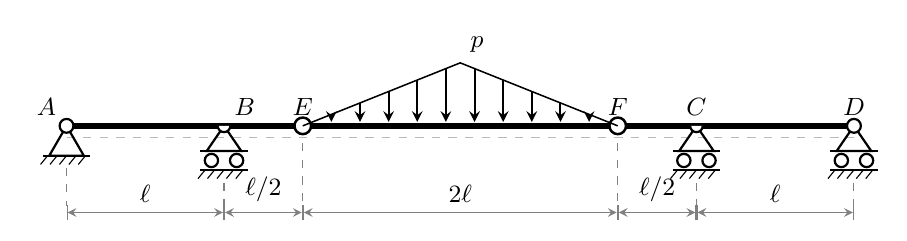
\begin{tikzpicture}[>=stealth, line width=0.8pt, font=\small,
	nodo/.style  = {circle, fill=white, draw=black,
		inner sep=0pt, minimum size=5pt, line width=0.8pt},
	cint/.style  = {circle, fill=white, draw=black,
		inner sep=0pt, minimum size=6pt, line width=0.9pt},
	richiam/.style = {thin, gray, dashed},
	]
	
	%% ── Parametri geometrici ─────────────────────────────────────────────────
	%% Unità: L = ell.  Posizioni:
	%%   A=0, B=L, E=1.5L, mez=2.5L, F=3.5L, C=4L, D=5L
	\def\L{2.00}     % ell
	\def\tw{0.22}    \def\thA{0.38}  \def\thR{0.32}
	\def\sr{0.08}    \def\bw{0.16}   \def\gw{0.30}
	\def\yd{-1.10}   % quota quotatura
	
	%% Posizioni nodi
	\pgfmathsetmacro{\xB}{\L}
	\pgfmathsetmacro{\xE}{1.5*\L}
	\pgfmathsetmacro{\xMez}{2.5*\L}   % mezzeria EF
	\pgfmathsetmacro{\xF}{3.5*\L}
	\pgfmathsetmacro{\xC}{4*\L}
	\pgfmathsetmacro{\xD}{5*\L}
	
	%% ── Trave ────────────────────────────────────────────────────────────────
	\draw[line width=2.2pt](0,0)--(\xD,0);
	
	%% ── Fibre inferiori ──────────────────────────────────────────────────────
	\draw[line width=0.6pt, dashed, gray!55](0,-0.15)--(\xD,-0.15);
	
	%% ── Etichette nodi ───────────────────────────────────────────────────────
	\node[above left =0.04]at(0,0){$A$};
	\node[above right=0.04]at(\xB,0){$B$};
	\node[above=0.12]at(\xE,0){$E$};
	\node[above=0.12]at(\xF,0){$F$};
	\node[above=0.04]at(\xC,0){$C$};
	\node[above=0.04]at(\xD,0){$D$};
	
	%% ── Cerniera A ───────────────────────────────────────────────────────────
	\draw(0,0)--++(-\tw,-\thA)--++(2*\tw,0)--cycle;
	\draw(-\gw,-\thA)--(\gw,-\thA);
	\foreach \x in {-0.24,-0.12,0,0.12,0.24}
	\draw[thin](\x,-\thA)--++(-.09,-.11);
	\node[nodo]at(0,0){};
	
	%% ── Appoggio intermedio B ────────────────────────────────────────────────
	\draw(\xB,0)--++(-\tw,-\thR)--++(2*\tw,0)--cycle;
	\draw(\xB-\gw,-\thR)--(\xB+\gw,-\thR);
	\draw(\xB-\bw,-\thR-0.12)circle(2.4pt);
	\draw(\xB+\bw,-\thR-0.12)circle(2.4pt);
	\draw(\xB-\gw,-\thR-0.24)--(\xB+\gw,-\thR-0.24);
	\foreach \x in {-0.24,-0.12,0,0.12,0.24}
	\draw[thin](\xB+\x,-\thR-0.24)--++(-.09,-.11);
	\fill[white](\xB-\sr,0)arc(180:360:\sr)--cycle;
	\draw(\xB-\sr,0)arc(180:360:\sr);
	
	%% ── Appoggio intermedio C ────────────────────────────────────────────────
	\draw(\xC,0)--++(-\tw,-\thR)--++(2*\tw,0)--cycle;
	\draw(\xC-\gw,-\thR)--(\xC+\gw,-\thR);
	\draw(\xC-\bw,-\thR-0.12)circle(2.4pt);
	\draw(\xC+\bw,-\thR-0.12)circle(2.4pt);
	\draw(\xC-\gw,-\thR-0.24)--(\xC+\gw,-\thR-0.24);
	\foreach \x in {-0.24,-0.12,0,0.12,0.24}
	\draw[thin](\xC+\x,-\thR-0.24)--++(-.09,-.11);
	\fill[white](\xC-\sr,0)arc(180:360:\sr)--cycle;
	\draw(\xC-\sr,0)arc(180:360:\sr);
	
	%% ── Carrello D ───────────────────────────────────────────────────────────
	\draw(\xD,0)--++(-\tw,-\thR)--++(2*\tw,0)--cycle;
	\draw(\xD-\gw,-\thR)--(\xD+\gw,-\thR);
	\draw(\xD-\bw,-\thR-0.12)circle(2.4pt);
	\draw(\xD+\bw,-\thR-0.12)circle(2.4pt);
	\draw(\xD-\gw,-\thR-0.24)--(\xD+\gw,-\thR-0.24);
	\foreach \x in {-0.24,-0.12,0,0.12,0.24}
	\draw[thin](\xD+\x,-\thR-0.24)--++(-.09,-.11);
	\node[nodo]at(\xD,0){};
	
	%% ── Cerniere interne E e F ───────────────────────────────────────────────
	\node[cint]at(\xE,0){};
	\node[cint]at(\xF,0){};
	
	%% ── Carico triangolare su EF ─────────────────────────────────────────────
	%% p(z) = (p/ell)*z  per 0<=z<=ell,  p(z)= p*(2-z/ell) per ell<=z<=2*ell
	%% ell = L,  altezza massima = hP
	\def\hP{0.80}   % altezza grafica picco p (cm)
	\def\nArr{11}   % numero di frecce
	
	%% contorno del diagramma di carico (linea superiore)
	\draw[line width=0.55pt,black]
	(\xE,0)
	-- (\xMez,\hP)
	-- (\xF,0);
	
	%% frecce verticali distribuite
	\foreach \k in {0,1,...,\nArr}{
		\pgfmathsetmacro{\t}{\k/\nArr}           % t in [0,1], x in [xE, xF]
		\pgfmathsetmacro{\xx}{\xE + \t*2*\L}      % x globale
		% intensità: tenda con picco in t=0.5
		\pgfmathsetmacro{\hh}{\hP*(1 - abs(2*\t - 1))}
		\ifdim\hh pt > 0.06pt
		\draw[->,>=stealth,line width=0.7pt](\xx,\hh)--(\xx,0.05);
		\fi}
	
	%% etichetta p
	\node[font=\small,above right=0.02]at(\xMez,\hP){$p$};
	
	%% ── Quotatura ─────────────────────────────────────────────────────────────
	\draw[richiam](0,-\thA-0.15)--(0,\yd+0.08);
	\draw[richiam](\xB,-\thR-0.40)--(\xB,\yd+0.08);
	\draw[richiam](\xE,-0.22)--(\xE,\yd+0.08);
	\draw[richiam](\xF,-0.22)--(\xF,\yd+0.08);
	\draw[richiam](\xC,-\thR-0.40)--(\xC,\yd+0.08);
	\draw[richiam](\xD,-\thR-0.40)--(\xD,\yd+0.08);
	
	\draw[thin,gray,|<->|](0,\yd)--(\xB,\yd);
	\node[font=\small,above=0.04]at(0.5*\xB,\yd){$\ell$};
	
	\draw[thin,gray,|<->|](\xB,\yd)--(\xE,\yd);
	\node[font=\small,above]at(0.5*\xB+0.5*\xE,\yd){$\ell/2$};
	
	\draw[thin,gray,|<->|](\xE,\yd)--(\xF,\yd);
	\node[font=\small,above]at(0.5*\xE+0.5*\xF,\yd){$2\ell$};
	
	\draw[thin,gray,|<->|](\xF,\yd)--(\xC,\yd);
	\node[font=\small,above]at(0.5*\xF+0.5*\xC,\yd){$\ell/2$};
	
	\draw[thin,gray,|<->|](\xC,\yd)--(\xD,\yd);
	\node[font=\small,above]at(0.5*\xC+0.5*\xD,\yd){$\ell$};
	
\end{tikzpicture}
\caption{Trave di Gerber su quattro appoggi ($n_a=4$, $n_e=5$,
	$n_c=2$): cerniera in $A$, appoggi continui in $B$ e $C$,
	carrello in $D$, cerniere interne in $E$ e $F$.
	Luci: $AB = CD = \ell$, $BE = FC = \ell/2$, $EF = 2\ell$.
	La campata portata $EF$ è soggetta a un carico trasversale
	triangolare di intensità massima $p$ nella sezione di mezzeria
	e nulla agli estremi $E$ e $F$.}
\label{fig:gerber_esempio_schema}
\end{figure}
%%%%%%%%%%%%%%%%%%%%%%%%%%%%%%%%%%%%%%%%%%%
\medskip
\noindent\textbf{1.~Classificazione.}
Il sistema ha $n_a = 4$ appoggi, $n_e = 5$ elementi e $n_c = 2$
cerniere interne, con grado di iperstaticità
\[
g_{\mathscr{i}} = (n_a - 2) - n_c = 2 - 2 = 0.
\]
Il sistema è \emph{isostatico}. Per assenza di carichi orizzontali
la reazione in $A$ è nulla e la forza normale è ovunque zero:
$N \equiv 0$.

La topologia è ad albero: la campata $EF$, delimitata dalle due
cerniere interne, è la \emph{campata portata}; le campate $ABE$
e $FCD$ sono le \emph{campate portanti}. La soluzione procede in
cascata: si analizza prima $EF$, poi $ABE$ e $FCD$.

\medskip
\noindent\textbf{2.~Campata portata $EF$.}
La campata $EF$ è una trave semplicemente appoggiata di luce $2\ell$,
vincolata in $E$ e $F$ dalle cerniere interne. Il carico totale vale
$p\ell$ (area del triangolo di base $2\ell$ e altezza $p$).
Per la simmetria del carico rispetto alla mezzeria di $EF$, le
reazioni alle cerniere sono uguali:
\[
V_E = V_F = \frac{p\ell}{2}.
\]
Introducendo l'ascissa $z$ con origine in $E$, il taglio e il
momento si ottengono per integrazione diretta. Nella prima metà
($0 \le z \le \ell$):
\[
T(z) = \frac{p\ell}{2} - \frac{p\,z^2}{2\ell},
\qquad
M(z) = \frac{p\ell}{2}\,z - \frac{p\,z^3}{6\ell}.
\]
Il taglio è \emph{parabolico} e si annulla in mezzeria ($z = \ell$);
il momento è \emph{cubico} e raggiunge il valore massimo in mezzeria:
\[
M\!\left(\ell\right) = \frac{p\ell^2}{2} - \frac{p\ell^2}{6}
= \frac{p\ell^2}{3}.
\]
Nella seconda metà i diagrammi si ottengono per antisimmetria ($T$)
e simmetria ($M$) rispetto alla mezzeria.
%%%%%%%%%%%%%%%%%%%%%%%%%%%%%%%%%%%%%%%%%%%
\begin{figure}[htbp]
\centering
\resizebox{0.80\textwidth}{!}{%
	\begin{tikzpicture}[
		trave/.style   = {line width=2.0pt, line cap=round, line join=round, black},
		terra/.style   = {line width=0.8pt, black},
		fibra/.style   = {line width=0.60pt, dashed, gray!55, line cap=round},
		reaz/.style    = {->, >=stealth, line width=1.0pt, black},
		diag/.style    = {line width=0.90pt, black},
		hatch/.style   = {line width=0.28pt, gray!60},
		nodo/.style    = {circle, fill=white, draw=black,
			inner sep=0pt, minimum size=5pt, line width=0.8pt},
		cint/.style    = {circle, fill=white, draw=black,
			inner sep=0pt, minimum size=6pt, line width=0.9pt},
		segno/.style   = {circle, draw=black, fill=white, inner sep=0pt,
			minimum size=9pt, font=\tiny, line width=0.55pt},
		etcirc/.style  = {circle, draw=black, fill=white, inner sep=2pt,
			font=\small, line width=0.7pt},
		lab/.style     = {font=\small},
		tlab/.style    = {font=\scriptsize},
		richiam/.style = {thin, gray!55, dashed},
		]
		
		\def\L{1.80}
		\pgfmathsetmacro{\xB}{\L}
		\pgfmathsetmacro{\xE}{1.5*\L}
		\pgfmathsetmacro{\xMid}{2.5*\L}
		\pgfmathsetmacro{\xF}{3.5*\L}
		\pgfmathsetmacro{\xC}{4.0*\L}
		\pgfmathsetmacro{\xD}{5.0*\L}
		
		\def\yel{1.90}
		\def\hP{0.75}
		\def\hT{0.85}
		\pgfmathsetmacro{\hTh}{\hT*0.5}
		\def\hM{1.20}
		\pgfmathsetmacro{\hMq}{\hM*0.75}
		
		\def\tw{0.22}  \def\thA{0.38}  \def\thR{0.32}
		\def\sr{0.08}  \def\bw{0.16}   \def\gw{0.30}
		
		\def\yT{-2.40}
		\def\yM{-6.00}
		
		%% ── Macro vincoli ────────────────────────────────────────────────────────
		\newcommand{\cernA}[1]{%
			\draw[terra](#1,0)--++(-\tw,-\thA)--++(2*\tw,0)--cycle;
			\draw[terra]({#1-\gw},{-\thA})--({#1+\gw},{-\thA});
			\foreach \x in {-0.22,-0.11,0,0.11,0.22}
			\draw[very thin,black]({#1+\x},{-\thA})--++(-.09,-.11);
			\node[nodo]at(#1,0){};}
		
		\newcommand{\carrR}[1]{%
			\draw[terra](#1,0)--++(-\tw,-\thR)--++(2*\tw,0)--cycle;
			\draw[terra]({#1-\gw},{-\thR})--({#1+\gw},{-\thR});
			\draw[terra]({#1-\bw},{-\thR-0.12})circle(2.4pt);
			\draw[terra]({#1+\bw},{-\thR-0.12})circle(2.4pt);
			\draw[terra]({#1-\gw},{-\thR-0.24})--({#1+\gw},{-\thR-0.24});
			\foreach \x in {-0.22,-0.11,0,0.11,0.22}
			\draw[very thin,black]({#1+\x},{-\thR-0.24})--++(-.09,-.11);}
		
		\newcommand{\carrSemi}[1]{\carrR{#1}%
			\fill[white]({#1-\sr},0)arc(180:360:\sr)--cycle;
			\draw[terra]({#1-\sr},0)arc(180:360:\sr);}
		
		\newcommand{\carrNodo}[1]{\carrR{#1}\node[nodo]at(#1,0){};}
		
		\newcommand{\strutturaBase}{%
			\draw[trave](0,0)--(\xD,0);
			\draw[fibra](0,-0.14)--(\xD,-0.14);
			\cernA{0}\carrSemi{\xB}\carrSemi{\xC}\carrNodo{\xD}
			\node[cint]at(\xE,0){};\node[cint]at(\xF,0){};}
		
		\newcommand{\nodiTM}{%
			\node[lab,above left=0.04]at(0,0){$A$};
			\node[lab,above right=0.04]at(\xB,0){$B$};
			\node[lab,above=0.06]at(\xE,0){$E$};
			\node[lab,above=0.06]at(\xF,0){$F$};
			\node[lab,above=0.04]at(\xC,0){$C$};
			\node[lab,above=0.04]at(\xD,0){$D$};}
		
		%% macro hatch verticale: righe verticali da y1 a y2, x in [xa,xb], passo 0.18
		\newcommand{\hatchV}[4]{%  #1=xa #2=xb #3=y1 #4=y2
			\pgfmathsetmacro{\hstep}{0.18}
			\foreach \xi in {#1,#2,...,#3}
			\draw[hatch](\xi,#4)--(\xi,#4);}% placeholder, replaced below
		
		%% ════════════════════════════════════════════════════════════════════════
		%% RIGA 1 — SCHEMA CON REAZIONI
		%% ════════════════════════════════════════════════════════════════════════
		\begin{scope}[yshift=0cm]
			\draw[trave](0,0)--(\xE,0);
			\draw[fibra](0,-0.15)--(\xE,-0.15);
			\cernA{0}\carrSemi{\xB}\node[cint]at(\xE,0){};
			\node[lab,above left=0.04]at(0,0){$A$};
			\node[lab,above left]at(\xB,0){$B$};
			\node[lab,above right]at(\xE,0){$E$};
			
			\draw[trave](\xE,\yel)--(\xF,\yel);
			\draw[fibra](\xE,{\yel-0.15})--(\xF,{\yel-0.15});
			\node[cint]at(\xE,\yel){};\node[cint]at(\xF,\yel){};
			\node[lab,above=0.10]at(\xE,\yel){$E$};
			\node[lab,above=0.10]at(\xF,\yel){$F$};
			\draw[richiam](\xE,0.08)--(\xE,{\yel-0.08});
			\draw[richiam](\xF,0.08)--(\xF,{\yel-0.08});
			
			\draw[line width=0.55pt](\xE,\yel)--(\xMid,{\yel+\hP})--(\xF,\yel);
			\foreach \k in {0,1,...,12}{
				\pgfmathsetmacro{\t}{\k/12.0}
				\pgfmathsetmacro{\xx}{\xE+\t*(\xMid-\xE)}
				\pgfmathsetmacro{\hh}{\hP*\t}
				\ifdim\hh pt>0.04pt\draw[->,>=stealth,line width=0.65pt](\xx,{\yel+\hh})--(\xx,{\yel+0.06});\fi}
			\foreach \k in {0,1,...,12}{
				\pgfmathsetmacro{\t}{\k/12.0}
				\pgfmathsetmacro{\xx}{\xMid+\t*(\xF-\xMid)}
				\pgfmathsetmacro{\hh}{\hP*(1-\t)}
				\ifdim\hh pt>0.04pt\draw[->,>=stealth,line width=0.65pt](\xx,{\yel+\hh})--(\xx,{\yel+0.06});\fi}
			\node[tlab,above=0.04]at(\xMid,{\yel+\hP}){$p$};
			
			\draw[reaz](\xE,{\yel-0.70})--(\xE,{\yel-0.08});
			\node[tlab,left=0.03]at(\xE,{\yel-0.38}){$\tfrac{p\ell}{2}$};
			\draw[reaz](\xF,{\yel-0.70})--(\xF,{\yel-0.08});
			\node[tlab,right=0.03]at(\xF,{\yel-0.38}){$\tfrac{p\ell}{2}$};
			
			\draw[reaz](\xE,0.70)--(\xE,0.08);
			\node[tlab,left=0.03]at(\xE,0.38){$\tfrac{p\ell}{2}$};
			
			\draw[reaz](0,0.55)--(0,0.08);
			\node[tlab,above]at(0,0.60){$\tfrac{p\ell}{4}$};
			\draw[reaz](\xB,0.08)--(\xB,0.72);
			\node[tlab,above]at(\xB,0.78){$\tfrac{3p\ell}{4}$};
			
			\draw[trave](\xF,0)--(\xD,0);
			\draw[fibra](\xF,-0.15)--(\xD,-0.15);
			\node[cint]at(\xF,0){};\carrSemi{\xC}\carrNodo{\xD}
			\node[lab,above left]at(\xF,0){$F$};
			\node[lab,above right]at(\xC,0){$C$};
			\node[lab,above right]at(\xD,0){$D$};
			
			\draw[reaz](\xF,0.70)--(\xF,0.08);
			\node[tlab,right=0.03]at(\xF,0.38){$\tfrac{p\ell}{2}$};
			\draw[reaz](\xC,0.08)--(\xC,0.72);
			\node[tlab,above]at(\xC,0.78){$\tfrac{3p\ell}{4}$};
			\draw[reaz](\xD,0.55)--(\xD,0.08);
			\node[tlab,above]at(\xD,0.60){$\tfrac{p\ell}{4}$};
		\end{scope}
		
		%% ════════════════════════════════════════════════════════════════════════
		%% RIGA 2 — DIAGRAMMA T
		%% ════════════════════════════════════════════════════════════════════════
		\begin{scope}[yshift=\yT cm]
			
			%% AB (sotto, negativo)
			\fill[gray!15](0,-\hTh)rectangle(\xB,0);
			\begin{scope}
				\clip(0,-\hTh)rectangle(\xB,0);
				\foreach \xi in {0,0.18,...,2.0}
				\draw[hatch](\xi,-\hTh)--(\xi,0);
			\end{scope}
			\draw[diag](0,0)--(0,-\hTh)--(\xB,-\hTh)--(\xB,\hT); % salto B incluso
			
			%% BE (sopra, positivo)
			\fill[gray!15](\xB,0)rectangle(\xE,\hT);
			\draw[diag](\xB,0)--(\xB,\hT)--(\xE,\hT);
			
			%% EF prima metà (sopra, positivo)
			\fill[gray!15]
			plot[domain=0:1,samples=60]({\xE+\x*\L},{\hT*(1-\x*\x)})
			--(\xMid,0)--(\xE,0)--cycle;
			\draw[diag](\xE,\hT)
			plot[domain=0:1,samples=60]({\xE+\x*\L},{\hT*(1-\x*\x)});
			
			%% hatch BE + EF prima metà
			\begin{scope}
				\clip(\xB,0)--(\xB,\hT)
				--plot[domain=0:1,samples=60]({\xE+\x*\L},{\hT*(1-\x*\x)})
				--(\xB,0)--cycle;
				\foreach \xi in {1.8,1.98,...,4.7}
				\draw[hatch](\xi,-0.05)--(\xi,{\hT+0.05});
			\end{scope}
			
			%% EF seconda metà (sotto, negativo) — curva da (xMid,0) a (xF,-hT)
			\fill[gray!15](\xMid,0)
			plot[domain=0:1,samples=30]({\xMid+\x*\L},{\hT*(\x*\x-2*\x)})
			--(\xF,0)--cycle;
			\begin{scope}
				\clip(\xMid,0)
				plot[domain=0:1,samples=30]({\xMid+\x*\L},{\hT*(\x*\x-2*\x)})
				--(\xF,0)--cycle;
				\foreach \xi in {4.5,4.68,...,6.5}
				\draw[hatch](\xi,-\hT)--(\xi,0);
			\end{scope}
			\draw[diag](\xMid,0)
			plot[domain=0:1,samples=30]({\xMid+\x*\L},{\hT*(\x*\x-2*\x)});
			
			%% FC (sotto, negativo)
			\fill[gray!15](\xF,-\hT)rectangle(\xC,0);
			\begin{scope}
				\clip(\xF,-\hT)rectangle(\xC,0);
				\foreach \xi in {6.3,6.48,...,7.4}
				\draw[hatch](\xi,-\hT)--(\xi,0);
			\end{scope}
			\draw[diag](\xF,-\hT)--(\xC,-\hT)--(\xC,\hTh);
			
			%% CD (sopra, positivo)
			\fill[gray!15](\xC,0)rectangle(\xD,\hTh);
			\begin{scope}
				\clip(\xC,0)rectangle(\xD,\hTh);
				\foreach \xi in {7.2,7.38,...,9.2}
				\draw[hatch](\xi,0)--(\xi,\hTh);
			\end{scope}
			\draw[diag](\xC,\hTh)--(\xD,\hTh)--(\xD,0);
			
			%% salto F e chiusura
			%\draw[diag](\xF,-\hT)--(\xF,0);
			
			%% struttura sopra
			\strutturaBase
			\node[lab,above left]at(0,0){$A$};
			\node[lab,above left]at(\xB,0){$B$};
			\node[lab,below]at(\xE,0){$E$};
			\node[lab,above]at(\xF,0){$F$};
			\node[lab,above left]at(\xC,0){$C$};
			\node[lab,above right]at(\xD,0){$D$};
			
			%% etichette valori
			\node[tlab,below]at({0.5*\xB},-\hTh){$\dfrac{p\ell}{4}$};
			\node[tlab,above]at({0.5*(\xB+\xE)},\hT){$\dfrac{p\ell}{2}$};
			\node[tlab,below]at({0.5*(\xF+\xC)},-\hT){$\dfrac{p\ell}{2}$};
			\node[tlab,above]at({0.5*(\xC+\xD)},\hTh){$\dfrac{p\ell}{4}$};
			
			%% cerchietti ±
			\node[segno]at({0.5*\xB},{-\hTh*0.52}){$-$};
			%\node[segno]at({0.5*(\xB+\xE)},{\hT*0.52}){$+$};
			\node[segno]at({\xE+0.*\L},{\hT*0.52}){$+$};
			\node[segno]at({\xMid+1.*\L},{-\hT*0.52}){$-$};
			%\node[segno]at({0.5*(\xF+\xC)},{-\hT*0.52}){$-$};
			\node[segno]at({0.5*(\xC+\xD)},{\hTh*0.52}){$+$};
			
			\node[etcirc]at({0.5*\xD},{-\hT-0.60}){$T$};
		\end{scope}
		
		%% ════════════════════════════════════════════════════════════════════════
		%% RIGA 3 — DIAGRAMMA M
		%% ════════════════════════════════════════════════════════════════════════
		\begin{scope}[yshift=\yM cm]
			
			%% AB (sopra, hogging) — triangolo
			\fill[gray!15](0,0)--(\xB,\hMq)--(\xB,0)--cycle;
			\begin{scope}
				\clip(0,0)--(\xB,\hMq)--(\xB,0)--cycle;
				\foreach \xi in {0,0.18,...,2.0}
				\draw[hatch](\xi,0)--(\xi,\hMq);
			\end{scope}
			\draw[diag](0,0)--(\xB,\hMq);
			%\draw[diag](\xB,0)--(\xB,\hMq);
			
			%% BE (sopra, hogging) — triangolo
			\fill[gray!15](\xB,0)--(\xB,\hMq)--(\xE,0)--cycle;
			\begin{scope}
				\clip(\xB,0)--(\xB,\hMq)--(\xE,0)--cycle;
				\foreach \xi in {1.8,1.98,...,3.0}
				\draw[hatch](\xi,0)--(\xi,\hMq);
			\end{scope}
			\draw[diag](\xB,\hMq)--(\xE,0);
			\node[tlab,above=0.02]at(\xB,\hMq){$\dfrac{p\ell^2}{4}$};
			
			%% EF prima metà (sotto, sagging) — cubica da (xE,0) a (xMid,-hM)
			\fill[gray!15](\xE,0)
			plot[domain=0:1,samples=30]({\xE+\x*\L},{-\hM*(3*\x-\x*\x*\x)/2})
			--(\xMid,0)--cycle;
			\begin{scope}
				\clip(\xE,0)
				plot[domain=0:1,samples=30]({\xE+\x*\L},{-\hM*(3*\x-\x*\x*\x)/2})
				--(\xMid,0)--cycle;
				\foreach \xi in {2.7,2.88,...,4.7}
				\draw[hatch](\xi,-\hM)--(\xi,0);
			\end{scope}
			\draw[diag](\xE,0)
			plot[domain=0:1,samples=30]({\xE+\x*\L},{-\hM*(3*\x-\x*\x*\x)/2});
			
			%% EF seconda metà (sotto, sagging) — cubica da (xMid,-hM) a (xF,0)
			\fill[gray!15](\xMid,-\hM)
			plot[domain=0:1,samples=30]
			({\xMid+\x*\L},{-\hM*(3*(1-\x)-(1-\x)*(1-\x)*(1-\x))/2})
			--(\xMid,0)--cycle;
			\begin{scope}
				\clip(\xMid,-\hM)
				plot[domain=0:1,samples=30]
				({\xMid+\x*\L},{-\hM*(3*(1-\x)-(1-\x)*(1-\x)*(1-\x))/2})
				--(\xMid,0)--cycle;
				\foreach \xi in {4.5,4.68,...,6.5}
				\draw[hatch](\xi,-\hM)--(\xi,0);
			\end{scope}
			\draw[diag](\xMid,{-\hM})
			plot[domain=0:1,samples=30]
			({\xMid+\x*\L},{-\hM*(3*(1-\x)-(1-\x)*(1-\x)*(1-\x))/2});
			\node[tlab,above=0.04]at(\xMid,{-\hM}){$\dfrac{p\ell^2}{3}$};
			
			%% FC (sopra, hogging) — triangolo
			\fill[gray!15](\xF,0)--(\xC,\hMq)--(\xC,0)--cycle;
			\begin{scope}
				\clip(\xF,0)--(\xC,\hMq)--(\xC,0)--cycle;
				\foreach \xi in {6.3,6.48,...,7.4}
				\draw[hatch](\xi,0)--(\xi,\hMq);
			\end{scope}
			\draw[diag](\xF,0)--(\xC,\hMq);
			%\draw[diag](\xC,0)--(\xC,\hMq);
			
			%% CD (sopra, hogging) — triangolo
			\fill[gray!15](\xC,0)--(\xC,\hMq)--(\xD,0)--cycle;
			\begin{scope}
				\clip(\xC,0)--(\xC,\hMq)--(\xD,0)--cycle;
				\foreach \xi in {7.2,7.38,...,9.2}
				\draw[hatch](\xi,0)--(\xi,\hMq);
			\end{scope}
			\draw[diag](\xC,\hMq)--(\xD,0);
			%\node[tlab,above=0.02]at(\xC,\hMq){$\dfrac{p\ell^2}{4}$};
			\node[tlab,above=0.04]at(\xC,\hMq){$\dfrac{p\ell^2}{4}$};
			
			%% struttura sopra
			%\strutturaBase\nodiTM
			\strutturaBase
			\node[lab,above left]at(0,0){$A$};
			\node[lab,above]at(\xB,0){$B$};
			\node[lab,above]at(\xE,0){$E$};
			\node[lab,above]at(\xF,0){$F$};
			\node[lab,above]at(\xC,0){$C$};
			\node[lab,above right]at(\xD,0){$D$};
			
			\node[etcirc]at({0.5*\xD},{-\hM-0.60}){$M$};
		\end{scope}
		
	\end{tikzpicture}
}%
\caption{Trave di Gerber: schema delle reazioni (\emph{prima riga}),
	taglio $T$ (\emph{seconda riga}) e momento $M$ (\emph{terza riga}).
	Le reazioni $V_A=V_D=p\ell/4$ verso il basso indicano che i perni $A$ e $D$
	trattengono la trave. Il taglio è emisimmetrico; il momento è simmetrico,
	nullo in $E$ e $F$, con massimo $p\ell^2/3$ (sagging) a mezzeria di $EF$
	e valore $p\ell^2/4$ (hogging) agli appoggi $B$ e $C$.}
\label{fig:gerber_esempio_diagrammi}
\end{figure}
%%%%%%%%%%%%%%%%%%%%%%%%%%%%%%%%%%%%%%%%%%%

\medskip
\noindent\textbf{3.~Campate portanti $ABE$ e $FCD$.}
Le reazioni $V_E = V_F = p\ell/2$ agiscono come forze concentrate
verso il basso alle cerniere $E$ e $F$, trasmesse per contatto
alle campate portanti (\FIGref{fig:gerber_esempio_diagrammi}\,a). Per la simmetria dello schema è sufficiente
analizzare $ABE$; i risultati si estendono a $FCD$ per speculare.

La campata $ABE$ è una trave isostatica (cerniera in $A$, carrello
in $B$) di luce $3\ell/2$, con forza concentrata $p\ell/2$ verso il
basso applicata in $E$. L'equilibrio alla rotazione intorno ad $A$ fornisce:
\[
\sum M_A = 0\colon \quad
V_B \cdot \ell - \frac{p\ell}{2} \cdot \frac{3\ell}{2} = 0
\quad\Longrightarrow\quad
V_B = \frac{3p\ell}{4}.
\]
L'equilibrio alla traslazione verticale fornisce:
\[
\sum V = 0\colon \quad
V_A + V_B = \frac{p\ell}{2}
\quad\Longrightarrow\quad
V_A = -\frac{p\ell}{4}.
\]
Il segno negativo di $V_A$ indica che il perno in $A$ deve
\emph{trattenere} la trave verso il basso: la campata $ABE$ tende
a sollevarsi in corrispondenza di $A$ per effetto del carico
trasmesso in $E$.

Su $ABE$ non vi sono carichi distribuiti, quindi i diagrammi sono
lineari a tratti. Il taglio è uniforme su ciascun tratto:
$T = V_A = -p\ell/4$ su $AB$ e $T = p\ell/2$ su $BE$.
Il momento è lineare, nullo alle cerniere $A$ e $E$, con valore
\[
M(B) = V_A \cdot \ell = -\frac{p\ell^2}{4}
\]
all'appoggio $B$ (momento negativo).
Per simmetria, su $FCD$: $V_C = 3p\ell/4$, $V_D = -p\ell/4$,
$M(C) = -p\ell^2/4$.

\medskip
\noindent\textbf{4.~Commento sui diagrammi.}
I diagrammi di $T$ e $M$ sono illustrati nella
\FIGref{fig:gerber_esempio_diagrammi}.
Introducendo l'ascissa $x$ con origine nell'asse di simmetria
della travata (mezzeria di $EF$), lo schema di carico è
simmetrico rispetto a $x = 0$: ne consegue che le
\emph{reazioni agli appoggi sono simmetriche}
($V_A = V_D$, $V_B = V_C$) e che i diagrammi ereditano
la stessa proprietà.

Il \emph{taglio} è una \emph{funzione dispari}:
$T(-x) = -T(x)$, con andamento parabolico su $EF$
e uniforme sui tratti portanti.
Il \emph{momento} è una \emph{funzione pari}:
$M(-x) = M(x)$.
Queste proprietà sono conseguenza diretta della simmetria
dello schema e del carico; la simmetria strutturale nelle
sue implicazioni statiche, cinematiche e costitutive è
trattata sistematicamente nel Vol.~II.

Il momento è nullo alle cerniere interne $E$ e $F$
(condizione imposta dalla presenza delle cerniere stesse)
e agli appoggi di estremità $A$ e $D$ (cerniera e carrello).
Assume il valore massimo assoluto $p\ell^2/3$ a mezzeria
di $EF$ (momento positivo, fibre inferiori tese) e il
valore $-p\ell^2/4$ agli appoggi intermedi $B$ e $C$
(momento negativo, fibre superiori tese).


%............................................................................................................................
\subsection{Travi continue}
\label{subsec:travi_continue}
%............................................................................................................................

Una \emph{trave continua}\index{trave!continua|textbf} è un sistema di $n_e$ travi
disposte in serie lungo uno stesso asse, collegate tra
loro con nodi rigidi e vincolate al suolo in più punti.
Il numero di appoggi è $n_a = n_e + 1$ se la trave è
vincolata anche alle due estremità; in generale
$n_a \geq 2$.

\paragraph{Classificazione.}
Con la configurazione minima di vincoli esterni ---
una cerniera e $(n_a - 1)$ carrelli a asse verticale
--- si ha:
\begin{equation}\label{eq:class_trave_continua}
m_{\text{est}} = n_a + 1, \qquad
m_{\text{int}} = 3(n_e - 1), \qquad
\nu = 3n_e - m = -(n_a - 2).
\end{equation}
Il sistema è iperstatico di grado $g_{\mathscr{i}} = n_a - 2$,
pari al numero di appoggi \emph{intermedi} (quelli diversi
dai due di estremità).

La \FIGref{fig:trave_continua} illustra una trave
continua a tre campate con la classificazione corrispondente.


%%%%%%%%%%%%%%%%%%%%%%%%%%%%%%%%%%%%%%%%%%%
\begin{figure}[htbp]
\centering
\begin{tikzpicture}[>=Stealth, line width=0.8pt, font=\small,
	nodo/.style={circle, fill=white, draw=black,
		inner sep=0pt, minimum size=5pt, line width=0.8pt},
	etasta/.style={circle, draw=black, fill=white,
		inner sep=1pt, font=\scriptsize, line width=0.6pt},
	richiam/.style={thin, gray, dashed}]
	
	\def\L{2.8}    % lunghezza campata
	\def\tw{0.22}  % semi-larghezza triangolo
	\def\thA{0.38} % altezza triangolo cerniera (A)
	\def\thR{0.32} % altezza triangolo carrello
	\def\rn{0.08}  % raggio semicerchio al vertice
	\def\bw{0.16}  % semi-distanza cerchietti carrello
	\def\gw{0.30}  % semi-larghezza barra di terreno
	\def\yd{-1.10} % quota linee di misura
	
	%% ── Trave ────────────────────────────────────────────────────
	\draw[line width=2.2pt] (0,0) -- ({3*\L},0);
	
	%% ── Etichette nodi ───────────────────────────────────────────
	\node[above=0.05] at (0,0)      {$A$};
	\node[above=0.05] at ({\L},0)   {$B$};
	\node[above=0.05] at ({2*\L},0) {$C$};
	\node[above=0.05] at ({3*\L},0) {$D$};
	
	%% ── Numerazione campate ───────────────────────────────────────
	\node[etasta] at ({0.5*\L},  0.38) {$1$};
	\node[etasta] at ({1.5*\L},  0.38) {$2$};
	\node[etasta] at ({2.5*\L},  0.38) {$3$};
	
	%%═══════════════════════════════════════════════════════════════
	%% CERNIERA in A
	%%═══════════════════════════════════════════════════════════════
	\draw[line width=0.8pt]
	(0,0)--++(-\tw,-\thA)--++(2*\tw,0)--cycle;
	\draw[line width=0.8pt]({-\gw},{-\thA})--({\gw},{-\thA});
	\foreach \x in {-0.24,-0.12,0,0.12,0.24}
	\draw[thin]({\x},{-\thA})--++(-.09,-.11);
	\node[nodo] at (0,0){};
	
	%%═══════════════════════════════════════════════════════════════
	%% APPOGGIO INTERMEDIO in B
	%%═══════════════════════════════════════════════════════════════
	\draw[line width=0.8pt]
	({\L},0)--++(-\tw,-\thR)--++(2*\tw,0)--cycle;
	\draw[line width=0.8pt]
	({\L-\gw},{-\thR})--({\L+\gw},{-\thR});
	\draw[line width=0.8pt]({\L-\bw},{-\thR-0.12}) circle(2.4pt);
	\draw[line width=0.8pt]({\L+\bw},{-\thR-0.12}) circle(2.4pt);
	\draw[line width=0.8pt]
	({\L-\gw},{-\thR-0.24})--({\L+\gw},{-\thR-0.24});
	\foreach \x in {-0.24,-0.12,0,0.12,0.24}
	\draw[thin]({\L+\x},{-\thR-0.24})--++(-.09,-.11);
	\draw[line width=0.8pt, fill=white]
	({\L-\rn},0) arc(180:360:\rn) -- cycle;
	
	%%═══════════════════════════════════════════════════════════════
	%% APPOGGIO INTERMEDIO in C
	%%═══════════════════════════════════════════════════════════════
	\draw[line width=0.8pt]
	({2*\L},0)--++(-\tw,-\thR)--++(2*\tw,0)--cycle;
	\draw[line width=0.8pt]
	({2*\L-\gw},{-\thR})--({2*\L+\gw},{-\thR});
	\draw[line width=0.8pt]({2*\L-\bw},{-\thR-0.12}) circle(2.4pt);
	\draw[line width=0.8pt]({2*\L+\bw},{-\thR-0.12}) circle(2.4pt);
	\draw[line width=0.8pt]
	({2*\L-\gw},{-\thR-0.24})--({2*\L+\gw},{-\thR-0.24});
	\foreach \x in {-0.24,-0.12,0,0.12,0.24}
	\draw[thin]({2*\L+\x},{-\thR-0.24})--++(-.09,-.11);
	\draw[line width=0.8pt, fill=white]
	({2*\L-\rn},0) arc(180:360:\rn) -- cycle;
	
	%%═══════════════════════════════════════════════════════════════
	%% CARRELLO in D
	%%═══════════════════════════════════════════════════════════════
	\draw[line width=0.8pt]
	({3*\L},0)--++(-\tw,-\thR)--++(2*\tw,0)--cycle;
	\draw[line width=0.8pt]
	({3*\L-\gw},{-\thR})--({3*\L+\gw},{-\thR});
	\draw[line width=0.8pt]({3*\L-\bw},{-\thR-0.12}) circle(2.4pt);
	\draw[line width=0.8pt]({3*\L+\bw},{-\thR-0.12}) circle(2.4pt);
	\draw[line width=0.8pt]
	({3*\L-\gw},{-\thR-0.24})--({3*\L+\gw},{-\thR-0.24});
	\foreach \x in {-0.24,-0.12,0,0.12,0.24}
	\draw[thin]({3*\L+\x},{-\thR-0.24})--++(-.09,-.11);
	\node[nodo] at ({3*\L},0){};
	
	%%═══════════════════════════════════════════════════════════════
	%% QUOTATURA
	%%═══════════════════════════════════════════════════════════════
	\draw[richiam](0,      {-\thA-0.15})  -- (0,      {\yd+0.08});
	\draw[richiam]({\L},   {-\thR-0.40})  -- ({\L},   {\yd+0.08});
	\draw[richiam]({2*\L}, {-\thR-0.40})  -- ({2*\L}, {\yd+0.08});
	\draw[richiam]({3*\L}, {-\thR-0.40})  -- ({3*\L}, {\yd+0.08});
	
	\draw[thin, gray, |<->|] (0,{\yd}) -- ({\L},{\yd});
	\node[above=0.04, font=\small] at ({0.5*\L},{\yd}) {$\ell_1$};
	\draw[thin, gray, |<->|] ({\L},{\yd}) -- ({2*\L},{\yd});
	\node[above=0.04, font=\small] at ({1.5*\L},{\yd}) {$\ell_2$};
	\draw[thin, gray, |<->|] ({2*\L},{\yd}) -- ({3*\L},{\yd});
	\node[above=0.04, font=\small] at ({2.5*\L},{\yd}) {$\ell_3$};
	
\end{tikzpicture}
\caption{Trave continua a tre campate di luci $\ell_1$, $\ell_2$,
	$\ell_3$ ($n_e = 3$, $n_a = 4$): cerniera in $A$,
	appoggi intermedi in $B$ e $C$, carrello in $D$.
	Il cerchio in $A$ e $D$ indica il perno della
	connessione; il semicerchio in $B$ e $C$ indica
	che la trave scorre sull'appoggio senza interruzione
	della continuità rotazionale.
	Gradi di libertà $n = 9$, vincoli $m = 11$,
	grado di iperstaticità $g_{\mathscr{i}} = 2$
	pari al numero di appoggi intermedi.}
\label{fig:trave_continua}
\end{figure}
%%%%%%%%%%%%%%%%%%%%%%%%%%%%%%%%%%%%%%%%%%%

\paragraph{Comportamento esterno e interno.}
La trave continua è un sistema ad \emph{albero} (senza
maglie chiuse): le travi sono collegate in serie e la
topologia è aperta. Questo implica che il sistema è
\emph{internamente isostatico}: note le reazioni al
suolo, le caratteristiche della sollecitazione si
determinano univocamente per equilibrio, elemento per
elemento. Tutta l'iperstaticità è quindi \emph{esterna}:
il grado di iperstaticità globale coincide con quello
esterno, $g_{\mathscr{i}} = g_{\mathscr{i}}^{\text{est}} = n_a - 2$.

\paragraph{Lettura cinematica duale.}
Il grado di iperstaticità $g_{\mathscr{i}} = n_a - 2$
corrisponde, sul versante cinematico, a $n_a - 2$
condizioni di compatibilità che i cedimenti vincolari
devono soddisfare affinché la trave ammetta una
configurazione congruente. Un cedimento differenziale
generico degli appoggi intermedi è cinematicamente
incompatibile: la trave reagisce sviluppando reazioni
iperstatiche che ristabiliscono la congruenza.

\paragraph{Sistema principale.}
Per un'analisi iperstatica si individua un sistema
principale\index{sistema principale} isostatico rimuovendo $g_{\mathscr{i}}$
vincoli. Le scelte più comuni sono:
\begin{itemize}[noitemsep]
\item rimozione degli appoggi intermedi: le
incognite iperstatiche $\chi_j$\index{iperstaticita@iperstaticità!incognita iperstatica} sono le reazioni
verticali degli appoggi rimossi;
\item inserimento di cerniere sugli appoggi
intermedi: le incognite $\chi_j$ sono i momenti
di continuità $M$ in corrispondenza degli appoggi.
\end{itemize}
In entrambi i casi i diagrammi di $N$, $T$, $M$ si
esprimono come sovrapposizione della soluzione
particolare e delle autosoluzioni, con la determinazione
delle $\chi_j$ rinviata al Vol.~II.



%............................................................................................................................
\paragraph{Esempio.}
\label{par:esempio_trave_continua}
%............................................................................................................................

Con riferimento allo schema della \FIGref{fig:tc_schema},
si considera la trave continua a tre campate di luce uguale
$\ell$: cerniera in $A$, appoggi intermedi in $B$ e $C$,
carrello in $D$. I carichi applicati sono: un carico distribuito
uniforme $p$ verso il basso sulla campata $AB$,  una coppia concentrata $\mu$ antioraria
applicata alla sezione  $C$, e una forza concentrata $F$ verso il basso alla mezzeria
della campata $CD$.

%%%%%%%%%%%%%%%%%%%%%%%%%%%%%%%%%%%%%%%%%%%%%%%%%%%%%%%%%%%%%%
\begin{figure}[htbp]
\centering
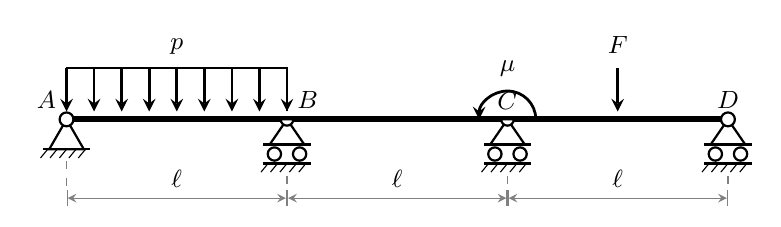
\begin{tikzpicture}[>=stealth, line width=0.8pt, font=\small,
	nodo/.style={circle, fill=white, draw=black,
		inner sep=0pt, minimum size=5pt, line width=0.8pt},
	carr/.style={->, >=stealth, line width=1.0pt, black},
	quota/.style={thin, gray, |<->|},
	richiam/.style={thin, gray, dashed},
	]
	
	\def\L{2.80}    % lunghezza campata
	\def\tw{0.22}   % semi-larghezza triangolo
	\def\thA{0.38}  % altezza triangolo cerniera A
	\def\thR{0.32}  % altezza triangolo carrello
	\def\rn{0.08}   % raggio semicerchio appoggi intermedi B, C
	\def\bw{0.16}   % semi-distanza ruote carrello
	\def\gw{0.30}   % semi-larghezza barra di terra
	\def\yd{-1.00}  % quota linee di misura
	
	%% ── Trave ────────────────────────────────────────────────────────────────
	\draw[line width=2.2pt](0,0)--({3*\L},0);
	
	%% ── Fibre inferiori ──────────────────────────────────────────────────────
	%\draw[line width=0.6pt, dashed, gray!55](0,-0.15)--({3*\L},-0.15);
	
	%% ── Etichette nodi ───────────────────────────────────────────────────────
	\node[above left =0.04]at(0,0){$A$};
	\node[above right=0.04]at({\L},0){$B$};
	\node[above=-0.08]at({2*\L},0){$C$};
	\node[above=0.04]at({3*\L},0){$D$};
	
	%% ── Cerniera A ───────────────────────────────────────────────────────────
	\draw(0,0)--++(-\tw,-\thA)--++(2*\tw,0)--cycle;
	\draw({-\gw},{-\thA})--(\gw,{-\thA});
	\foreach \x in {-0.24,-0.12,0,0.12,0.24}
	\draw[thin](\x,{-\thA})--++(-.09,-.11);
	\node[nodo]at(0,0){};
	
	%% ── Appoggio intermedio B (semicerchio = continuità rotazionale) ──────────
	\draw({\L},0)--++(-\tw,-\thR)--++(2*\tw,0)--cycle;
	\draw({\L-\gw},{-\thR})--({\L+\gw},{-\thR});
	\draw({\L-\bw},{-\thR-0.12})circle(2.4pt);
	\draw({\L+\bw},{-\thR-0.12})circle(2.4pt);
	\draw({\L-\gw},{-\thR-0.24})--({\L+\gw},{-\thR-0.24});
	\foreach \x in {-0.24,-0.12,0,0.12,0.24}
	\draw[thin]({\L+\x},{-\thR-0.24})--++(-.09,-.11);
	\draw[fill=white]({\L-\rn},0) arc(180:360:\rn)--cycle;
	
	%% ── Appoggio intermedio C (semicerchio = continuità rotazionale) ──────────
	\draw({2*\L},0)--++(-\tw,-\thR)--++(2*\tw,0)--cycle;
	\draw({2*\L-\gw},{-\thR})--({2*\L+\gw},{-\thR});
	\draw({2*\L-\bw},{-\thR-0.12})circle(2.4pt);
	\draw({2*\L+\bw},{-\thR-0.12})circle(2.4pt);
	\draw({2*\L-\gw},{-\thR-0.24})--({2*\L+\gw},{-\thR-0.24});
	\foreach \x in {-0.24,-0.12,0,0.12,0.24}
	\draw[thin]({2*\L+\x},{-\thR-0.24})--++(-.09,-.11);
	\draw[fill=white]({2*\L-\rn},0) arc(180:360:\rn)--cycle;
	
	%% ── Carrello D ───────────────────────────────────────────────────────────
	\draw({3*\L},0)--++(-\tw,-\thR)--++(2*\tw,0)--cycle;
	\draw({3*\L-\gw},{-\thR})--({3*\L+\gw},{-\thR});
	\draw({3*\L-\bw},{-\thR-0.12})circle(2.4pt);
	\draw({3*\L+\bw},{-\thR-0.12})circle(2.4pt);
	\draw({3*\L-\gw},{-\thR-0.24})--({3*\L+\gw},{-\thR-0.24});
	\foreach \x in {-0.24,-0.12,0,0.12,0.24}
	\draw[thin]({3*\L+\x},{-\thR-0.24})--++(-.09,-.11);
	\node[nodo]at({3*\L},0){};
	
	%% ── Carico distribuito p su AB ───────────────────────────────────────────
	\draw[line width=0.5pt](0,0.10)--(0,0.65)--({\L},0.65)--({\L},0.10);
	\foreach \k in {0,1,2,3,4,5,6,7,8}{
		\pgfmathsetmacro{\xk}{\k*(\L/8.0)}
		\draw[carr]({\xk},0.65)--({\xk},0.10);}
	\node[font=\small,above]at({0.5*\L},0.70){$p$};
	
	%% ── Coppia μ in C: semicerchio sopra, convessità verso l'alto ────────────
	\def\rmu{0.36}
	\draw[->,>=stealth,line width=1.0pt]({2*\L+\rmu},0) arc(0:180:\rmu);
	\node[font=\small,above]at({2*\L},{\rmu+0.05}){$\mu$};
	
	%% ── Forza F a mezzeria CD ────────────────────────────────────────────────
	\draw[carr]({2.5*\L},0.65)--({2.5*\L},0.10);
	\node[font=\small,above]at({2.5*\L},0.70){$F$};
	
	%% ── Quotatura ────────────────────────────────────────────────────────────
	\draw[richiam](0,{-\thA-0.15})--(0,{\yd+0.08});
	\draw[richiam]({\L},{-\thR-0.40})--({\L},{\yd+0.08});
	\draw[richiam]({2*\L},{-\thR-0.40})--({2*\L},{\yd+0.08});
	\draw[richiam]({3*\L},{-\thR-0.40})--({3*\L},{\yd+0.08});
	\draw[quota](0,{\yd})--({\L},{\yd});
	\node[font=\small,above=0.04]at({0.5*\L},{\yd}){$\ell$};
	\draw[quota]({\L},{\yd})--({2*\L},{\yd});
	\node[font=\small,above=0.04]at({1.5*\L},{\yd}){$\ell$};
	\draw[quota]({2*\L},{\yd})--({3*\L},{\yd});
	\node[font=\small,above=0.04]at({2.5*\L},{\yd}){$\ell$};
	
\end{tikzpicture}
\caption{Trave continua a tre campate di uguale luce $\ell$:
	carico uniformemente distribuito $p$ sul tratto $AB$,
	coppia concentrata $\mu$ nella sezione $C$,
	forza concentrata $F$ a mezzeria del tratto $CD$.
	Il cerchio in $A$ e $D$ indica il perno; il semicerchio in $B$ e $C$
	indica che la trave scorre sull'appoggio senza interruzione
	della continuità rotazionale.}
\label{fig:tc_schema}
\end{figure}
%%%%%%%%%%%%%%%%%%%%%%%%%%%%%%%%%%%%%%%%%%%%%%%%%%%%%%%%%%%%%%
\medskip
\noindent\textbf{Classificazione.}
Per forze orizzontali la struttura è isostatica: l'unica
reazione orizzontale disponibile è $H_A$ alla cerniera $A$.
In assenza di carichi orizzontali $H_A = 0$, e la forza
normale è nulla ovunque: $N = 0$.

Per forze trasversali le reazioni incognite sono quattro
($V_A$, $V_B$, $V_C$, $V_D$), a fronte di due sole equazioni
di equilibrio utili ($\sum V = 0$ e $\sum M = 0$), con
grado di iperstaticità
\[
g_\mathscr{i} = 4 - 2 = n_a - 2 = 2,
\]
coerente con il conteggio generale già svolto.
La topologia è ad albero --- le tre campate sono in serie,
senza maglie chiuse --- per cui l'iperstaticità è interamente
esterna: $g_\mathscr{i}^{\mathrm{int}} = 0$,
$g_\mathscr{i}^{\mathrm{est}} = 2$.

\medskip
\noindent\textbf{Sistema principale.}
Si inserisce una cerniera interna in corrispondenza di
ciascun appoggio intermedio, in $B$ e in $C$, eliminando
la trasmissione del momento flettente in quei punti.
Le tre campate diventano travi semplicemente appoggiate e
completamente indipendenti; le incognite iperstatiche sono
i momenti di continuità:
\[
\chi_1 = M(B), \qquad \chi_2 = M(C).
\]
La soluzione si decompone nella sovrapposizione del
\emph{problema~0} (carichi assegnati, $\chi_1 = \chi_2 = 0$)
e delle due \emph{autosoluzioni}
($\chi_j = 1$, nessun carico esterno).

\medskip
\noindent\textbf{Problema~0.}
Carichi assegnati, $\chi_1 = \chi_2 = 0$.

Le tre campate si risolvono indipendentemente.
Poiché non vi sono carichi orizzontali, $N_0 = 0$ ovunque.

\medskip
\noindent\textit{Campata $AB$
(lunghezza $\ell$, carico uniforme $p$).}

Schema di trave appoggiata sotto carico uniforme;
per simmetria $V_A^{(0)} = V_B^{(0)} = p\ell/2$:
\[
T_0(z) = \frac{p\ell}{2} - pz, \qquad
M_0(z) = \frac{p\ell}{2}\,z - \frac{pz^2}{2},
\quad z \in [0,\ell] \text{ da } A.
\]
Il taglio si annulla a mezzeria; il momento è parabolico
con massimo
\[
M_0^{\max} = \frac{p\ell^2}{8} \quad \text{in } z = \ell/2.
\]

\medskip
\noindent\textit{Campata $BC$
(lunghezza $\ell$, coppia $\mu$ antioraria in $C$).}

Il tratto è privo di carichi distribuiti e di forze
concentrate. La coppia $\mu$, applicata all'estremità
destra sul lato della campata $BC$, è equilibrata
dalle sole reazioni agli appoggi. L'equilibrio dei
momenti rispetto a $B$ e quello delle forze verticali
forniscono:
\[
V_B^{(0)} = +\frac{\mu}{\ell}
\quad (\text{verso l'alto}), \qquad
V_C^{(0)} = -\frac{\mu}{\ell}
\quad (\text{verso il basso}).
\]
Il taglio è uniforme; il momento è lineare:
\[
T_0 = \frac{\mu}{\ell}, \qquad
M_0(z) = \frac{\mu}{\ell}\,z, \quad z \in [0,\ell) \text{ da } B.
\]
Il momento cresce da zero in $B$ fino a $\mu$ appena
prima di $C$; la coppia antioraria $\mu$ in $C$ produce
un salto $\Delta M = -\mu$ che riporta il momento al
valore nullo imposto dalla cerniera del sistema principale:
\[
M_0(C^+) = M_0(C^-) - \mu = \mu - \mu = 0.
\quad\checkmark
\]

\begin{oss}
Una coppia antioraria $\mu$ applicata in $z_0$ produce
un salto negativo del momento flettente:
$M(z_0^+) = M(z_0^-) - \mu$.
In questo esempio il salto riassorbe esattamente
il momento accumulato lungo la campata, restituendo
$M = 0$ alla sezione della cerniera in $C$.
La condizione del sistema principale è soddisfatta
non nonostante la coppia, ma \emph{grazie} ad essa:
è la posizione della coppia in corrispondenza
dell'appoggio che rende il diagramma di $M_0$
su $BC$ un triangolo rettangolo con vertice in $C^-$.
\end{oss}

\medskip
\noindent\textit{Campata $CD$
(lunghezza $\ell$, forza $F$ verso il basso a mezzeria).}

\noindent Per simmetria $V_C^{(0)} = V_D^{(0)} = F/2$:
\[
T_0(z) = \begin{cases}
+\dfrac{F}{2} & 0 \le z < \dfrac{\ell}{2}, \\[8pt]
-\dfrac{F}{2} & \dfrac{\ell}{2} < z \le \ell,
\end{cases}
\qquad
M_0(z) = \begin{cases}
\dfrac{F}{2}\,z & 0 \le z \le \dfrac{\ell}{2}, \\[8pt]
\dfrac{F}{2}(\ell - z) & \dfrac{\ell}{2} \le z \le \ell,
\end{cases}
\]
con $z \in [0,\ell]$ da $C$. Il diagramma di $M_0$ è
triangolare con colmo $F\ell/4$ alla mezzeria.

\medskip
\noindent\textbf{Autosoluzione~1.}
$\chi_1 = 1$, $\chi_2 = 0$, nessun carico esterno.

Si applica al sistema principale un momento unitario
in $B$. La cerniera in $C$ isola completamente la
campata $CD$: $M_1 = T_1 = 0$ su $CD$.
Il momento cresce linearmente da zero in $A$ all'unità
in $B$, poi decresce da uno in $B$ a zero in $C$:
\[
M_1 = \begin{cases}
z/\ell & z \in [0,\ell] \text{ su } AB, \\[4pt]
1 - z/\ell & z \in [0,\ell] \text{ su } BC, \\[4pt]
0 & \text{su } CD;
\end{cases}
\qquad
T_1 = \begin{cases}
+1/\ell & \text{su } AB, \\[4pt]
-1/\ell & \text{su } BC, \\[4pt]
0 & \text{su } CD.
\end{cases}
\]
Il diagramma di $M_1$ ha forma a \emph{tenda} con vertice
unitario in $B$ e zeri in $A$ e $C$.
%%%%%%%%%%%%%%%%%%%%%%%%%%%%%%%%%%%%%%%%%%%%%%%%%%%%%%%%%%%%%%
\begin{figure}[htbp]
\centering
\resizebox{\textwidth}{!}{%
	\begin{tikzpicture}[
		trave/.style  = {line width=2.0pt, line cap=round, line join=round, black},
		terra/.style  = {line width=0.8pt, black},
		fibra/.style  = {line width=0.65pt, dashed, gray!55, line cap=round},
		carr/.style   = {->, >=stealth, line width=1.0pt, black},
		diag/.style   = {line width=0.9pt, black},
		nodo/.style   = {circle, fill=white, draw=black,
			inner sep=0pt, minimum size=5pt, line width=0.8pt},
		cint/.style   = {circle, fill=white, draw=black,
			inner sep=0pt, minimum size=6.5pt, line width=1.0pt},
		segno/.style  = {circle, draw=black, fill=white, inner sep=0pt,
			minimum size=9pt, font=\tiny, line width=0.55pt},
		lab/.style    = {font=\small},
		tlab/.style   = {font=\small},
		]
		
		%% ── Parametri ────────────────────────────────────────────────────────────
		\def\Ls{1.80}
		\def\twi{0.20}  \def\thA{0.38}  \def\thR{0.30}
		\def\bww{0.13}  \def\gww{0.26}
		
		\def\TA{0.72}   \def\TB{0.28}   \def\TC{0.54}   % T_0
		\def\Ts{0.52}                                    % T_1, T_2
		\def\MA{1.00}   \def\MB{0.80}   \def\MC{0.65}   % M_0
		\def\Ms{1.05}                                    % M_1, M_2 (vertice)
		
		%% ── Macro vincoli ────────────────────────────────────────────────────────
		\newcommand{\cernieraA}{%
			\draw[terra](0,0)--++(-\twi,-\thA)--++(2*\twi,0)--cycle;
			\draw[terra]({-\gww},{-\thA})--(\gww,{-\thA});
			\foreach \xi in {-0.20,-0.10,0.00,0.10,0.20}
			\draw[very thin,black](\xi,{-\thA})--++(-0.09,-0.11);
			\node[nodo]at(0,0){};}
		
		\newcommand{\carrello}[1]{%
			\draw[terra](#1,0)--++(-\twi,-\thR)--++(2*\twi,0)--cycle;
			\draw[terra]({#1-\gww},{-\thR})--({#1+\gww},{-\thR});
			\draw[terra]({#1-\bww},{-\thR-0.13})circle(2.0pt);
			\draw[terra]({#1+\bww},{-\thR-0.13})circle(2.0pt);
			\draw[terra]({#1-\gww},{-\thR-0.26})--({#1+\gww},{-\thR-0.26});
			\foreach \xi in {-0.20,-0.10,0.00,0.10,0.20}
			\draw[very thin,black]({#1+\xi},{-\thR-0.26})--++(-0.09,-0.11);
			\node[nodo]at(#1,0){};}
		
		\newcommand{\traveVincoli}{%
			\draw[trave](0,0)--({3*\Ls},0);
			\cernieraA
			\carrello{\Ls}  \carrello{2*\Ls}  \carrello{3*\Ls}}
		
		%% Label nodi standard (above=0.04 per tutti)
		\newcommand{\nodiABCD}{%
			\node[lab,above=0.04]at(0,0){$A$};
			\node[lab,above=0.04]at({\Ls},0){$B$};
			\node[lab,above=0.04]at({2*\Ls},0){$C$};
			\node[lab,above=0.04]at({3*\Ls},0){$D$};}
		
		\newcommand{\traveVincoliCI}{%
			\traveVincoli
			\node[cint]at({\Ls},0){};
			\node[cint]at({2*\Ls},0){};}
		
		\newcommand{\fibraInf}{%
			\draw[fibra](0,-0.15)--({3*\Ls},-0.15);}
		
		%% ── Intestazioni di colonna ──────────────────────────────────────────────
		\node[lab,align=center]at({0.5*3*1.80},     1.10){\textbf{Problema 0}};
		\node[lab,align=center]at({7.0+0.5*3*1.80}, 1.10){\textbf{Problema 1}};
		\node[lab,align=center]at({14.0+0.5*3*1.80},1.10){\textbf{Problema 2}};
		
		%% ════════════════════════════════════════════════════════════════════════
		%% COLONNA 1 — Problema 0
		%% ════════════════════════════════════════════════════════════════════════
		
		%%─── (a) Schema ─────────────────────────────────────────────────────────
		\begin{scope}[xshift=0cm, yshift=0cm]
			\traveVincoliCI  \fibraInf
			%% etichette nodi (A a sinistra, B a destra)
			\node[lab,above left=0.04]at(0,0){$A$};
			\node[lab,above right=0.04]at({\Ls},0){$B$};
			\node[lab,above right=0.04]at({2*\Ls},0){$C$};
			\node[lab,above=0.04]at({3*\Ls},0){$D$};
			%% rettangolo delimitatore del carico p
			\draw[black,line width=0.5pt](0,0.07)--(0,0.52)--({1.80},0.52)--({1.80},0.07);
			\foreach \k in {0,1,2,3,4,5,6}{
				\pgfmathsetmacro{\xk}{\k*(1.80/6.0)}
				\draw[carr]({\xk},0.52)--({\xk},0.08);}
			\node[tlab,above]at({0.5*1.80},0.59){$p$};
			%% coppia μ in C: arco 180° CCW, convessità verso BC
			\draw[->,>=stealth,line width=0.85pt]({2*1.80},{0.24})arc(90:270:0.24);
			\node[tlab,right]at({2*1.80-0.50},0.25){$\mu$};
			\draw[carr]({2.5*1.80},0.52)--({2.5*1.80},0.07);
			\node[tlab,above]at({2.5*1.80},0.59){$F$};
			\node[lab]at({1.5*1.80},-0.95){$(a)$};
		\end{scope}
		
		%%─── (d) T_0  ──  fill → diag → struttura → etichette + cerchietti ──────
		\begin{scope}[xshift=0cm, yshift=-2.7cm]
			%% 1. fill
			\fill[gray!15](0,0)--(0,\TA)--({0.5*\Ls},0)--cycle;
			\fill[gray!15]({0.5*\Ls},0)--({\Ls},0)--({\Ls},{-\TA})--cycle;
			\fill[gray!15]({\Ls},0)rectangle({2*\Ls},\TB);
			\fill[gray!15]({2*\Ls},0)--({2*\Ls},\TC)--({2.5*\Ls},\TC)--({2.5*\Ls},0)--cycle;
			\fill[gray!15]({2.5*\Ls},0)--({2.5*\Ls},{-\TC})--({3*\Ls},{-\TC})--(3*\Ls,0)--cycle;
			%% 2. contorni diagramma
			\draw[diag](0,\TA)--({0.5*\Ls},0)--({\Ls},{-\TA});
			\draw[diag](0,0)--(0,\TA);
			\draw[diag]({\Ls},{-\TA})--({\Ls},\TB);          % salto B
			\draw[diag]({\Ls},0)--({\Ls},\TB);
			\draw[diag]({\Ls},\TB)--({2*\Ls},\TB);
			\draw[diag]({2*\Ls},0)--({2*\Ls},\TB);
			\draw[diag]({2*\Ls},\TB)--({2*\Ls},\TC);          % salto C
			\draw[diag]({2*\Ls},\TC)--({2.5*\Ls},\TC);
			\draw[diag]({2.5*\Ls},\TC)--({2.5*\Ls},{-\TC});   % gradino F
			\draw[diag]({2.5*\Ls},{-\TC})--({3*\Ls},{-\TC});
			\draw[diag]({3*\Ls},{-\TC})--({3*\Ls},0);
			%% 3. struttura (in primo piano)
			\traveVincoliCI  \fibraInf
			%\nodiABCD
			\node[lab,above left=0.04]at(0,0){$A$};
			\node[lab,above left=0.04]at({\Ls},0){$B$};
			\node[lab,above=0.04]at({2*\Ls},0){$C$};
			\node[lab,above=0.04]at({3*\Ls},0){$D$};
			
			%% 4. etichette valori
			\node[tlab,left]at(0,\TA){$\tfrac{p\ell}{2}$};
			\node[tlab,right]at({\Ls},{-\TA}){$\tfrac{p\ell}{2}$};
			\node[tlab,above]at({1.5*\Ls},\TB){$\tfrac{\mu}{\ell}$};
			\node[tlab,above]at({2.25*\Ls},\TC){$\tfrac{F}{2}$};
			\node[tlab,below]at({2.75*\Ls},{-\TC}){$\tfrac{F}{2}$};
			%% 5. cerchietti ±
			\node[segno]at({0.5*\Ls*0.35},{\TA*0.33}){$+$};   % AB sopra
			\node[segno]at({\Ls*0.85},{-\TA*0.33}){$-$};       % AB sotto
			\node[segno]at({1.5*\Ls},{\TB*0.52}){$+$};         % BC
			\node[segno]at({2.25*\Ls},{\TC*0.52}){$+$};        % CD prima metà
			\node[segno]at({2.75*\Ls},{-\TC*0.52}){$-$};       % CD seconda metà
			\node[lab]at({1.5*\Ls},-1.4){$(d)$};
		\end{scope}
		
		%%─── (g) M_0  ──  fill → diag → struttura → etichette ──────────────────
		\begin{scope}[xshift=0cm, yshift=-6.0cm]
			%% 1. fill
			\fill[gray!15](0,0)
			plot[domain=0:1,samples=22]({\x*1.80},{-1.00*4*\x*(1-\x)})--cycle;
			\fill[gray!15]({\Ls},0)--({2*\Ls},{-\MB})--({2*\Ls},0)--cycle;
			\fill[gray!15]({2*\Ls},0)--({2.5*\Ls},{-\MC})--({3*\Ls},0)--cycle;
			%% 2. contorni diagramma
			\draw[diag]plot[domain=0:1,samples=22]({\x*1.80},{-1.00*4*\x*(1-\x)});
			\draw[diag]({\Ls},0)--({2*\Ls},{-\MB});
			\draw[diag]({2*\Ls},{-\MB})--({2*\Ls},0);                              % lato dx BC
			\draw[dashed,gray!65,line width=0.70pt]({2*\Ls},{-\MB})--({2*\Ls},0); % salto C
			\draw[->,>=stealth,line width=0.55pt,gray!75]
			({2*\Ls+0.18},{-\MB*0.58})--({2*\Ls+0.18},-0.05);
			\draw[diag]({2*\Ls},0)--({2.5*\Ls},{-\MC})--({3*\Ls},0);
			%% 3. struttura
			\traveVincoliCI  \fibraInf
			\nodiABCD
			%% 4. etichette
			\node[tlab,above]at({0.5*1.80},{-\MA}){$\tfrac{p\ell^2}{8}$};
			\node[tlab,below right]at({2*\Ls},{-\MB}){$\mu$};
			%\node[tlab,right,gray!75]at({2*\Ls+0.20},{-\MB*0.55}){$\Delta M$};
			\node[tlab,above]at({2.5*\Ls},{-\MC}){$\tfrac{F\ell}{4}$};
			\node[lab]at({1.5*1.80},-0.90){$(g)$};
		\end{scope}
		
		%% ════════════════════════════════════════════════════════════════════════
		%% COLONNA 2 — Autosoluzione 1  (χ₁=1)
		%% ════════════════════════════════════════════════════════════════════════
		
		%%─── (b) Schema ─────────────────────────────────────────────────────────
		\begin{scope}[xshift=7.0cm, yshift=0cm]
			\traveVincoliCI  \fibraInf
			\nodiABCD
			%% coppia χ₁=1 in B: arco CW (sx, aperto a sx) + arco CCW (dx, aperto a dx)
			\def\rchi{0.20}   % raggio
			\def\dchi{0.20}   % offset dei centri da B  (= rchi → gli archi si sfiorano in B)
			%% SX (CW): centro a B-dchi, semicerchio sinistro, freccia in cima punta verso B
			\draw[->,>=stealth,line width=0.88pt]
			({1.80-\dchi},{-\rchi}) arc(270:90:\rchi);
			%% DX (CCW): centro a B+dchi, semicerchio destro, freccia in cima punta verso B
			\draw[->,>=stealth,line width=0.88pt]
			({1.80+\dchi},{-\rchi}) arc(-90:90:\rchi);
			\node[tlab,above=0.30]at({1.80},0){$\chi_1{=}1$};
			\node[lab]at({1.5*\Ls},-0.95){$(b)$};
		\end{scope}
		
		%%─── (e) T_1  ──  fill → diag → struttura → etichette + cerchietti ──────
		\begin{scope}[xshift=7.0cm, yshift=-2.7cm]
			%% 1. fill
			\fill[gray!15](0,0)rectangle({\Ls},\Ts);
			\fill[gray!15]({\Ls},{-\Ts})rectangle({2*\Ls},0);
			%% 2. contorni
			\draw[diag](0,0)--(0,\Ts)--({\Ls},\Ts);
			\draw[diag]({\Ls},0)--({\Ls},\Ts);
			\draw[diag]({\Ls},\Ts)--({\Ls},{-\Ts});          % salto B
			\draw[diag]({\Ls},{-\Ts})--({2*\Ls},{-\Ts});
			\draw[diag]({2*\Ls},0)--({2*\Ls},{-\Ts});
			\draw[diag]({2*\Ls},{-\Ts})--({2*\Ls},0);        % salto C
			%% 3. struttura
			\traveVincoliCI  \fibraInf
			%\nodiABCD
			\node[lab,above left=0.04]at(0,0){$A$};
			\node[lab,above right=0.04]at({\Ls},0){$B$};
			\node[lab,above=0.04]at({2*\Ls},0){$C$};
			\node[lab,above=0.04]at({3*\Ls},0){$D$};
			
			%% 4. etichette
			\node[tlab,above]at({0.5*\Ls},\Ts){$1/\ell$};
			\node[tlab,below]at({1.5*\Ls},{-\Ts}){$1/\ell$};
			%% 5. cerchietti ±
			\node[segno]at({0.5*\Ls},{\Ts*0.52}){$+$};
			\node[segno]at({1.5*\Ls},{-\Ts*0.52}){$-$};
			\node[lab]at({1.5*\Ls},-1.4){$(e)$};
		\end{scope}
		
		%%─── (h) M_1 : tenda in B  ──  SOPRA (negativo) ────────────────────────
		\begin{scope}[xshift=7.0cm, yshift=-6.0cm]
			%% 1. fill (sopra l'asse: M₁ < 0, fibra superiore tesa)
			\fill[gray!15](0,0)--({\Ls},\Ms)--({2*\Ls},0)--cycle;
			%% 2. contorno
			\draw[diag](0,0)--({\Ls},\Ms)--({2*\Ls},0);
			%% 3. struttura
			\traveVincoliCI  \fibraInf
			\nodiABCD
			%% 4. etichette
			\node[tlab,above]at({\Ls},\Ms){$1$};
			\node[lab]at({1.5*1.80},-0.90){$(h)$};
		\end{scope}
		
		%% ════════════════════════════════════════════════════════════════════════
		%% COLONNA 3 — Autosoluzione 2  (χ₂=1)
		%% ════════════════════════════════════════════════════════════════════════
		
		%%─── (c) Schema ─────────────────────────────────────────────────────────
		\begin{scope}[xshift=14.0cm, yshift=0cm]
			\traveVincoliCI  \fibraInf
			\nodiABCD
			%% coppia χ₂=1 in C: arco CW (sx) + arco CCW (dx)
			\def\rchi{0.20}   % raggio
			\def\dchi{0.20}   % offset dei centri da B  (= rchi → gli archi si sfiorano in B)
			%% SX (CW): centro a B-dchi, semicerchio sinistro, freccia in cima punta verso B
			\draw[->,>=stealth,line width=0.88pt]
			({2*1.80-\dchi},{-\rchi}) arc(270:90:\rchi);
			%% DX (CCW): centro a B+dchi, semicerchio destro, freccia in cima punta verso B
			\draw[->,>=stealth,line width=0.88pt]
			({2*1.80+\dchi},{-\rchi}) arc(-90:90:\rchi);
			\node[tlab,above=0.30]at({2*1.80},0){$\chi_2{=}1$};
			\node[lab]at({1.5*\Ls},-0.95){$(c)$};
		\end{scope}
		
		%%─── (f) T_2  ──  fill → diag → struttura → etichette + cerchietti ──────
		\begin{scope}[xshift=14.0cm, yshift=-2.7cm]
			%% 1. fill
			\fill[gray!15]({\Ls},0)rectangle({2*\Ls},\Ts);
			\fill[gray!15]({2*\Ls},{-\Ts})rectangle({3*\Ls},0);
			%% 2. contorni
			\draw[diag]({\Ls},0)--({\Ls},\Ts);              % salto B (0→+Ts)
			\draw[diag]({\Ls},\Ts)--({2*\Ls},\Ts);          % BC sopra
			\draw[diag]({2*\Ls},\Ts)--({2*\Ls},{-\Ts});     % salto C (+Ts→−Ts)
			\draw[diag]({2*\Ls},{-\Ts})--({3*\Ls},{-\Ts});  % CD sotto
			\draw[diag]({3*\Ls},{-\Ts})--({3*\Ls},0);       % salto D
			%% 3. struttura
			\traveVincoliCI  \fibraInf
			%\nodiABCD
			\node[lab,above=0.04 ]at(0,0){$A$};
			\node[lab,above left=0.04]at({\Ls},0){$B$};
			\node[lab,above right=0.04]at({2*\Ls},0){$C$};
			\node[lab,above=0.04]at({3*\Ls},0){$D$};
			%% 4. etichette
			\node[tlab,above]at({1.5*\Ls},\Ts){$1/\ell$};
			\node[tlab,below]at({2.5*\Ls},{-\Ts}){$1/\ell$};
			%% 5. cerchietti ±
			\node[segno]at({1.5*\Ls},{\Ts*0.52}){$+$};
			\node[segno]at({2.5*\Ls},{-\Ts*0.52}){$-$};
			\node[lab]at({1.5*\Ls},-1.4){$(f)$};
		\end{scope}
		
		%%─── (i) M_2 : tenda in C  ──  SOPRA (negativo) ────────────────────────
		\begin{scope}[xshift=14.0cm, yshift=-6.0cm]
			%% 1. fill (sopra l'asse)
			\fill[gray!15]({\Ls},0)--({2*\Ls},\Ms)--({3*\Ls},0)--cycle;
			%% 2. contorno
			\draw[diag]({\Ls},0)--({2*\Ls},\Ms)--({3*\Ls},0);
			%% 3. struttura
			\traveVincoliCI  \fibraInf
			\nodiABCD
			%% 4. etichette
			\node[tlab,above]at({2*\Ls},\Ms){$1$};
			\node[lab]at({1.5*1.80},-0.90){$(i)$};
		\end{scope}
		
		%% ── Etichette di riga ────────────────────────────────────────────────────
		\node[lab,rotate=90]at(-0.90, 0.00){Schema};
		\node[lab,rotate=90]at(-0.90,-2.70){$T$};
		\node[lab,rotate=90]at(-0.90,-6.0){$M$};
		
	\end{tikzpicture}
}%
\caption{Trave continua a tre campate uguali $\ell$: scomposizione secondo il
	metodo delle forze ($N\equiv 0$).
	\emph{Prima riga}: $(a)$~problema~$0$; $(b)$~autosoluzione~1 ($\chi_1=1$,
	momento unitario in $B$); $(c)$~autosoluzione~2 ($\chi_2=1$, momento unitario
	in $C$). I cerchietti indicano le cerniere interne del sistema principale;
	le fibre inferiori sono tratteggiate.
	\emph{Seconda riga}: diagrammi di $T$ con segno ($\oplus/\ominus$);
	$(d)$~$T_0$: lineare da $+p\ell/2$ a $-p\ell/2$ su $AB$, uniforme
	$\mu/\ell$ su $BC$, gradino $\pm F/2$ su $CD$; $(e)$~$T_1=\pm 1/\ell$;
	$(f)$~$T_2=\pm 1/\ell$.
	\emph{Terza riga}: diagrammi di $M$ ($M>0$ sotto, $M<0$ sopra);
	$(g)$~$M_0$: parabola ($p\ell^2/8$) su $AB$, triangolo con salto
	$\Delta M=-\mu$ in $C$ su $BC$, triangolo ($F\ell/4$) su $CD$;
	$(h)$~$M_1<0$: tenda con vertice unitario in $B$;
	$(i)$~$M_2<0$: tenda con vertice unitario in $C$.}
\label{fig:tc_scomposizione}
\end{figure}
%%%%%%%%%%%%%%%%%%%%%%%%%%%%%%%%%%%%%%%%%%%%%%%%%%%%%%%%%%%%%%

\medskip
\noindent\textbf{Autosoluzione~2.}
$\chi_2 = 1$, $\chi_1 = 0$, nessun carico esterno.

Analogo al precedente, con la tenda centrata in $C$;
la cerniera in $B$ isola questa volta la campata $AB$:
\[
M_2 = \begin{cases}
0 & \text{su } AB, \\[4pt]
z/\ell & z \in [0,\ell] \text{ su } BC, \\[4pt]
1 - z/\ell & z \in [0,\ell] \text{ su } CD;
\end{cases}
\qquad
T_2 = \begin{cases}
0 & \text{su } AB, \\[4pt]
+1/\ell & \text{su } BC, \\[4pt]
-1/\ell & \text{su } CD.
\end{cases}
\]

\medskip
\noindent\textbf{Struttura della soluzione.}
La soluzione generale è:
\begin{equation}
\label{eq:sovrapposizione_tc}
N = 0, \qquad
T = T_0 + \chi_1\,T_1 + \chi_2\,T_2, \qquad
M = M_0 + \chi_1\,M_1 + \chi_2\,M_2.
\end{equation}
Le incognite $\chi_1$ e $\chi_2$ si determinano imponendo
l'annullamento degli spostamenti relativi alle due cerniere
introdotte nel sistema principale (equazioni di congruenza
elastica): il sistema di due equazioni in due incognite
è sviluppato nel Vol.~II.

\begin{oss}
I diagrammi $M_1$ e $M_2$ a forma di tenda non
dipendono dai carichi applicati né dalle dimensioni
geometriche del problema, ma soltanto dalla scelta
del sistema principale. La localizzazione è una
conseguenza della topologia: il momento di continuità
in $B$ sollecita esclusivamente le campate adiacenti
$AB$ e $BC$, senza propagarsi alla campata $CD$
che la cerniera in $C$ isola; e specularmente
per $\chi_2$.
Nei sistemi iperstatici questo carattere \emph{locale}
delle autosoluzioni è una proprietà della scelta
del sistema principale, non del sistema originale:
la soluzione completa $M = M_0 + \chi_1 M_1 + \chi_2 M_2$
è globale e coinvolge tutte le campate attraverso
i valori delle incognite $\chi_j$.
\end{oss}







